% MIT 18.03 S2010：实际22份习题课；原题编号保留于标签。
% 题面和解答分别登记，来源/页码/哈希见research/recitations-coverage.json。
\originalchapter{习题课：一阶模型与复数响应}
本部分保留原课程习题课编号。公开文件为第1--5、7--11、13--19、21--25次，共22次；第6、12、20次为考试复习，第26次为课程复习，均没有本次清单中的公开题册。每题的中文题面与解答分列；“官方译审”表示核对过配套解答后重新组织推导，“编者补解（AI辅助）”表示补上官方没有提供的解答；“译审并补证（AI辅助）”表示在官方路线基础上补入论证。此稿由AI辅助撰写，独立第二读者为同模型另次审阅，不是MIT官方答案或外部专家鉴定。源文件所载日期均为2010年；文件作者未独立署名时沿用课程署名，不推测著作年份。原题提到的 Mathlet 在此用方程分析和自绘图落实，不声称运行过交互程序。

\originalsection{第1次习题课：自然增长、捕猎与对数（2月2日）}
\begin{exercise}\label{cw:rec01-1}
某非洲政府为剑羚捕猎制定政策。设种群自然增长率为 $k$，恒定捕猎量为每年 $a$ 只。选择变量与单位，建立种群模型。
\end{exercise}
\begin{solution}
以年为时间单位，$x(t)$ 为剑羚只数，$k$ 的单位为年$^{-1}$，$a$ 为只/年。短时间内增加 $kx\Delta t$ 只、捕猎 $a\Delta t$ 只，除以 $\Delta t$ 并取极限得 $\dot x=kx-a$。两端均为只/年。通常模型取 $k>0,a\ge0$，只在 $x\ge0$ 时有种群意义。
\par\noindent{\small 依据：官方译审并补证（AI辅助）。}
\end{solution}

\begin{exercise}\label{cw:rec01-2}
上述模型中若 $a=0$，种群的倍增时间是多少？
\end{exercise}
\begin{solution}
由 $\dot x=kx$ 得 $x(t)=x(0)\ee^{kt}$。正初值及 $k>0$ 时，$\ee^{kT}=2$，故 $T=\log2/k$ 年。零种群没有倍增时间；$k\le0$ 时没有正向倍增。
\par\noindent{\small 依据：官方译审并补证（AI辅助）。}
\end{solution}

\begin{exercise}\label{cw:rec01-3}
求 $\dot x=kx-a$ 的通解。
\end{exercise}
\begin{solution}
$k\ne0$ 时令 $z=x-a/k$，则 $\dot z=kz$，故 $x=a/k+C\ee^{kt}$。以初值表示为 $x=a/k+(x_0-a/k)\ee^{kt}$。若 $k=0$，直接积分得 $x=x_0-at$。
\par\noindent{\small 依据：官方译审并补证（AI辅助）。}
\end{solution}

\begin{exercise}\label{cw:rec01-4}
直接核验上一题提出的解满足原微分方程。
\end{exercise}
\begin{solution}
$k\ne0$ 时 $\dot x=kC\ee^{kt}=k(a/k+C\ee^{kt})-a$；$k=0$ 时 $\dot x=-a$。此外代入 $t=0$ 得指定初值，故方程与初值同时满足。
\par\noindent{\small 依据：官方译审并补证（AI辅助）。}
\end{solution}

\begin{exercise}\label{cw:rec01-5}
找出模型的稳态（常值、平衡）解；检查单位，以及对 $k,a$ 的大小依赖是否符合种群含义。
\end{exercise}
\begin{solution}
令 $\dot x=0$ 得 $x_*=a/k$（$k\ne0$）。单位为只/年除以年$^{-1}$，即只；捕猎量越大，需要越大的自然种群才能抵消损失，增长率越大则所需平衡种群越小。若 $k=0,a>0$ 无平衡；若 $k=a=0$ 所有常值均为平衡。
\par\noindent{\small 依据：官方译审并补证（AI辅助）。}
\end{solution}

\begin{exercise}\label{cw:rec01-6}
画出平衡解及其他解，说明不稳定性。低于平衡的初值何时灭绝？特别地，初值为平衡的一半时，求灭绝时间。
\end{exercise}
\begin{solution}
取 $k>0,a>0$，有 $x-x_*=(x_0-x_*)\ee^{kt}$：高于平衡则增长，低于平衡则下降，故平衡不稳定。$0\le x_0<x_*$ 时解 $x(t_0)=0$ 得 $t_0=k^{-1}\log[a/(a-kx_0)]$；$x_0=x_*/2$ 时为 $\log2/k$。负值应截断为灭绝，而过大的正值亦超出无限资源模型的有效范围。图用无量纲量 $s=kt,X=kx/a$，曲线族 $X=1+(X_0-1)\ee^s$。\begin{center}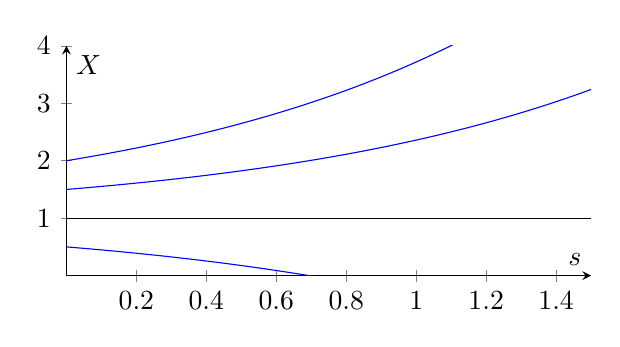
\begin{tikzpicture}\begin{axis}[width=.68\textwidth,height=4.5cm,axis lines=middle,xlabel={$s$},ylabel={$X$},samples=130,xmin=0,xmax=1.5,ymin=0,ymax=4]
\addplot[black,domain=0:1.5]{1};\foreach \c in {-1,-.5,.5,1}{\addplot[blue,domain=0:1.5]{1+\c*exp(x)};}\end{axis}\end{tikzpicture}\end{center}
\par\noindent{\small 依据：官方译审并补证（AI辅助）。}
\end{solution}

\originalsection{第2次习题课：方向场、等斜线、分界线与漏斗（2月4日）}
\begin{exercise}\label{cw:rec02-1}
对 $y'=x-2y$ 画若干等斜线，特别是零斜线，绘制方向场并画几条积分曲线。等斜线指 $F(x,y)=m$ 的点集。
\end{exercise}
\begin{solution}
等斜线为 $y=x/2-m/2$；零斜线为 $y=x/2$。每条等斜线上放斜率 $m$ 的短线段。由积分因子计算的曲线 $y=x/2-1/4+C\ee^{-2x}$ 可用于核对图。蓝线为解，虚线为零斜线与斜率 $1/2$ 的直线解。\begin{center}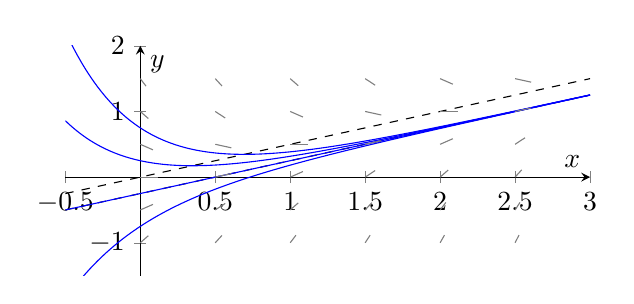
\begin{tikzpicture}\begin{axis}[width=.68\textwidth,height=4.5cm,axis lines=middle,xlabel={$x$},ylabel={$y$},samples=130,xmin=-.5,xmax=3,ymin=-1.5,ymax=2]
\addplot[dashed,domain=-.5:3]{x/2};\addplot[dashed,domain=-.5:3]{x/2-.25};\foreach \c in {-.5,0,.5,1}{\addplot[blue,domain=-.5:3]{x/2-.25+\c*exp(-2*x)};}\draw[gray](axis cs:0,-1)--(axis cs:0.05367,-0.89267);\draw[gray](axis cs:0,-0.5)--(axis cs:0.08485,-0.41515);\draw[gray](axis cs:0,0)--(axis cs:0.12000,0.00000);\draw[gray](axis cs:0,0.5)--(axis cs:0.08485,0.41515);\draw[gray](axis cs:0,1)--(axis cs:0.05367,0.89267);\draw[gray](axis cs:0,1.5)--(axis cs:0.03795,1.38616);\draw[gray](axis cs:0.5,-1)--(axis cs:0.54457,-0.88858);\draw[gray](axis cs:0.5,-0.5)--(axis cs:0.56656,-0.40015);\draw[gray](axis cs:0.5,0)--(axis cs:0.60733,0.05367);\draw[gray](axis cs:0.5,0.5)--(axis cs:0.60733,0.44633);\draw[gray](axis cs:0.5,1)--(axis cs:0.56656,0.90015);\draw[gray](axis cs:0.5,1.5)--(axis cs:0.54457,1.38858);\draw[gray](axis cs:1,-1)--(axis cs:1.03795,-0.88616);\draw[gray](axis cs:1,-0.5)--(axis cs:1.05367,-0.39267);\draw[gray](axis cs:1,0)--(axis cs:1.08485,0.08485);\draw[gray](axis cs:1,0.5)--(axis cs:1.12000,0.50000);\draw[gray](axis cs:1,1)--(axis cs:1.08485,0.91515);\draw[gray](axis cs:1,1.5)--(axis cs:1.05367,1.39267);\draw[gray](axis cs:1.5,-1)--(axis cs:1.53297,-0.88462);\draw[gray](axis cs:1.5,-0.5)--(axis cs:1.54457,-0.38858);\draw[gray](axis cs:1.5,0)--(axis cs:1.56656,0.09985);\draw[gray](axis cs:1.5,0.5)--(axis cs:1.60733,0.55367);\draw[gray](axis cs:1.5,1)--(axis cs:1.60733,0.94633);\draw[gray](axis cs:1.5,1.5)--(axis cs:1.56656,1.40015);\draw[gray](axis cs:2,-1)--(axis cs:2.02910,-0.88358);\draw[gray](axis cs:2,-0.5)--(axis cs:2.03795,-0.38616);\draw[gray](axis cs:2,0)--(axis cs:2.05367,0.10733);\draw[gray](axis cs:2,0.5)--(axis cs:2.08485,0.58485);\draw[gray](axis cs:2,1)--(axis cs:2.12000,1.00000);\draw[gray](axis cs:2,1.5)--(axis cs:2.08485,1.41515);\draw[gray](axis cs:2.5,-1)--(axis cs:2.52603,-0.88286);\draw[gray](axis cs:2.5,-0.5)--(axis cs:2.53297,-0.38462);\draw[gray](axis cs:2.5,0)--(axis cs:2.54457,0.11142);\draw[gray](axis cs:2.5,0.5)--(axis cs:2.56656,0.59985);\draw[gray](axis cs:2.5,1)--(axis cs:2.60733,1.05367);\draw[gray](axis cs:2.5,1.5)--(axis cs:2.60733,1.44633);\end{axis}\end{tikzpicture}\end{center}
\par\noindent{\small 依据：官方译审并补证（AI辅助）。}
\end{solution}

\begin{exercise}\label{cw:rec02-2}
图中似乎有一条直线积分曲线。判定 $y=mx+b$ 是否可能为解，并求 $m,b$。
\end{exercise}
\begin{solution}
代入得 $m=(1-2m)x-2b$。逐项比较：$m=1/2$、$b=-1/4$，所以 $y=x/2-1/4$ 确为解。
\par\noindent{\small 依据：官方译审并补证（AI辅助）。}
\end{solution}

\begin{exercise}\label{cw:rec02-3}
对一般方程 $y'=F(x,y)$，若一条直线是积分曲线，它与等斜线有何关系？说明本题中的情况。
\end{exercise}
\begin{solution}
直线 $y=mx+b$ 是解意味着在线上处处 $F(x,mx+b)=m$，故这条线属于斜率 $m$ 的等斜线；等斜线的其他分支未必也是解。本例直线解恰是整个 $m=1/2$ 等斜线。
\par\noindent{\small 依据：官方译审并补证（AI辅助）。}
\end{solution}

\begin{exercise}\label{cw:rec02-4}
图中各解在 $x\to\infty$ 时似乎互相渐近。先用方向场说明，为什么它们会被固定斜率的平行线夹住。
\end{exercise}
\begin{solution}
取 $y=x/2-m/2$。解与边界相遇时，相对边界的导数为 $m-1/2$。下边界取 $m>1/2$，解只能向内向上穿越；上边界取 $m<1/2$，解只能向内向下穿越。因此包含初值的这两条线围成正向不变带。任意窄带最终都会捕获解，因 $y-(x/2-1/4)=C\ee^{-2x}\to0$。
\par\noindent{\small 依据：官方译审并补证（AI辅助）。}
\end{solution}

\begin{exercise}\label{cw:rec02-5}
$y'=x-2y$ 的解在哪里有驻点？一条解最多有几个？哪些初值 $y(0)=y_0$ 会产生驻点？它是极小还是极大？用二阶导数检验。
\end{exercise}
\begin{solution}
驻点位于 $y=x/2$。通解中 $C=y_0+1/4$，$y'=1/2-2C\ee^{-2x}$，所以在全实轴上有驻点当且仅当 $C>0$，且唯一，位置为 $x_c=\frac12\log(4C)$。若只考察 $x\ge0$，要求 $y_0\ge0$（严格内部要求 $y_0>0$）。在驻点 $y''=1-2y'=1>0$，故是极小；驻点前后导数由负转正。
\par\noindent{\small 依据：官方译审并补证（AI辅助）。}
\end{solution}

\begin{exercise}\label{cw:rec02-6}
对另一方程 $y'=y^2-x^2$，画若干等斜线、方向场与几条解；原题建议用 Isoclines Mathlet。
\end{exercise}
\begin{solution}
等斜线为 $y^2-x^2=m$，$m=0$ 为 $y=\pm x$；在 $|y|>|x|$ 区域斜率为正，内部为负。图中灰色短线据 $F=y^2-x^2$ 绘制，虚线为零斜线。蓝线据数值积分只作示意；下两题用解析论证确定分界与漏斗，数值图不作为证明。\begin{center}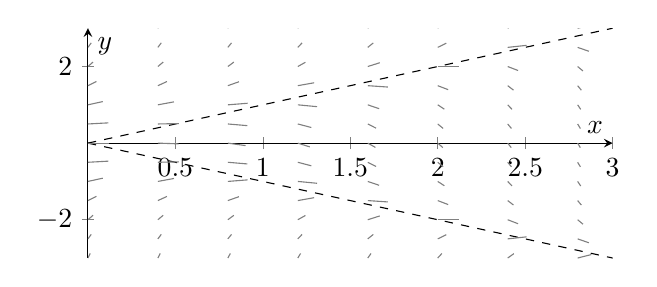
\begin{tikzpicture}\begin{axis}[width=.68\textwidth,height=4.5cm,axis lines=middle,xlabel={$x$},ylabel={$y$},samples=130,xmin=0,xmax=3,ymin=-3,ymax=3]
\addplot[dashed,domain=0:3]{x};\addplot[dashed,domain=0:3]{-x};\draw[gray](axis cs:0,-3)--(axis cs:0.01325,-2.88073);\draw[gray](axis cs:0,-2.5)--(axis cs:0.01896,-2.38151);\draw[gray](axis cs:0,-2)--(axis cs:0.02910,-1.88358);\draw[gray](axis cs:0,-1.5)--(axis cs:0.04874,-1.39034);\draw[gray](axis cs:0,-1)--(axis cs:0.08485,-0.91515);\draw[gray](axis cs:0,-0.5)--(axis cs:0.11642,-0.47090);\draw[gray](axis cs:0,0)--(axis cs:0.12000,0.00000);\draw[gray](axis cs:0,0.5)--(axis cs:0.11642,0.52910);\draw[gray](axis cs:0,1)--(axis cs:0.08485,1.08485);\draw[gray](axis cs:0,1.5)--(axis cs:0.04874,1.60966);\draw[gray](axis cs:0,2)--(axis cs:0.02910,2.11642);\draw[gray](axis cs:0,2.5)--(axis cs:0.01896,2.61849);\draw[gray](axis cs:0,3)--(axis cs:0.01325,3.11927);\draw[gray](axis cs:0.4,-3)--(axis cs:0.41349,-2.88076);\draw[gray](axis cs:0.4,-2.5)--(axis cs:0.41944,-2.38159);\draw[gray](axis cs:0.4,-2)--(axis cs:0.43024,-1.88387);\draw[gray](axis cs:0.4,-1.5)--(axis cs:0.45179,-1.39175);\draw[gray](axis cs:0.4,-1)--(axis cs:0.49188,-0.92282);\draw[gray](axis cs:0.4,-0.5)--(axis cs:0.51952,-0.48924);\draw[gray](axis cs:0.4,0)--(axis cs:0.51849,-0.01896);\draw[gray](axis cs:0.4,0.5)--(axis cs:0.51952,0.51076);\draw[gray](axis cs:0.4,1)--(axis cs:0.49188,1.07718);\draw[gray](axis cs:0.4,1.5)--(axis cs:0.45179,1.60825);\draw[gray](axis cs:0.4,2)--(axis cs:0.43024,2.11613);\draw[gray](axis cs:0.4,2.5)--(axis cs:0.41944,2.61841);\draw[gray](axis cs:0.4,3)--(axis cs:0.41349,3.11924);\draw[gray](axis cs:0.8,-3)--(axis cs:0.81425,-2.88085);\draw[gray](axis cs:0.8,-2.5)--(axis cs:0.82106,-2.38186);\draw[gray](axis cs:0.8,-2)--(axis cs:0.83423,-1.88499);\draw[gray](axis cs:0.8,-1.5)--(axis cs:0.86332,-1.39806);\draw[gray](axis cs:0.8,-1)--(axis cs:0.91291,-0.95935);\draw[gray](axis cs:0.8,-0.5)--(axis cs:0.91180,-0.54360);\draw[gray](axis cs:0.8,0)--(axis cs:0.90107,-0.06469);\draw[gray](axis cs:0.8,0.5)--(axis cs:0.91180,0.45640);\draw[gray](axis cs:0.8,1)--(axis cs:0.91291,1.04065);\draw[gray](axis cs:0.8,1.5)--(axis cs:0.86332,1.60194);\draw[gray](axis cs:0.8,2)--(axis cs:0.83423,2.11501);\draw[gray](axis cs:0.8,2.5)--(axis cs:0.82106,2.61814);\draw[gray](axis cs:0.8,3)--(axis cs:0.81425,3.11915);\draw[gray](axis cs:1.2,-3)--(axis cs:1.21574,-2.88104);\draw[gray](axis cs:1.2,-2.5)--(axis cs:1.22443,-2.38251);\draw[gray](axis cs:1.2,-2)--(axis cs:1.24366,-1.88823);\draw[gray](axis cs:1.2,-1.5)--(axis cs:1.29325,-1.42447);\draw[gray](axis cs:1.2,-1)--(axis cs:1.30984,-1.04833);\draw[gray](axis cs:1.2,-0.5)--(axis cs:1.27720,-0.59187);\draw[gray](axis cs:1.2,0)--(axis cs:1.26845,-0.09856);\draw[gray](axis cs:1.2,0.5)--(axis cs:1.27720,0.40813);\draw[gray](axis cs:1.2,1)--(axis cs:1.30984,0.95167);\draw[gray](axis cs:1.2,1.5)--(axis cs:1.29325,1.57553);\draw[gray](axis cs:1.2,2)--(axis cs:1.24366,2.11177);\draw[gray](axis cs:1.2,2.5)--(axis cs:1.22443,2.61749);\draw[gray](axis cs:1.2,3)--(axis cs:1.21574,3.11896);\draw[gray](axis cs:1.6,-3)--(axis cs:1.61841,-2.88142);\draw[gray](axis cs:1.6,-2.5)--(axis cs:1.63139,-2.38418);\draw[gray](axis cs:1.6,-2)--(axis cs:1.66845,-1.90144);\draw[gray](axis cs:1.6,-1.5)--(axis cs:1.71462,-1.53553);\draw[gray](axis cs:1.6,-1)--(axis cs:1.66476,-1.10103);\draw[gray](axis cs:1.6,-0.5)--(axis cs:1.64767,-0.61012);\draw[gray](axis cs:1.6,0)--(axis cs:1.64366,-0.11177);\draw[gray](axis cs:1.6,0.5)--(axis cs:1.64767,0.38988);\draw[gray](axis cs:1.6,1)--(axis cs:1.66476,0.89897);\draw[gray](axis cs:1.6,1.5)--(axis cs:1.71462,1.46447);\draw[gray](axis cs:1.6,2)--(axis cs:1.66845,2.09856);\draw[gray](axis cs:1.6,2.5)--(axis cs:1.63139,2.61582);\draw[gray](axis cs:1.6,3)--(axis cs:1.61841,3.11858);\draw[gray](axis cs:2,-3)--(axis cs:2.02353,-2.88233);\draw[gray](axis cs:2,-2.5)--(axis cs:2.04874,-2.39034);\draw[gray](axis cs:2,-2)--(axis cs:2.12000,-2.00000);\draw[gray](axis cs:2,-1.5)--(axis cs:2.05954,-1.60419);\draw[gray](axis cs:2,-1)--(axis cs:2.03795,-1.11384);\draw[gray](axis cs:2,-0.5)--(axis cs:2.03092,-0.61595);\draw[gray](axis cs:2,0)--(axis cs:2.02910,-0.11642);\draw[gray](axis cs:2,0.5)--(axis cs:2.03092,0.38405);\draw[gray](axis cs:2,1)--(axis cs:2.03795,0.88616);\draw[gray](axis cs:2,1.5)--(axis cs:2.05954,1.39581);\draw[gray](axis cs:2,2)--(axis cs:2.12000,2.00000);\draw[gray](axis cs:2,2.5)--(axis cs:2.04874,2.60966);\draw[gray](axis cs:2,3)--(axis cs:2.02353,3.11767);\draw[gray](axis cs:2.4,-3)--(axis cs:2.43539,-2.88534);\draw[gray](axis cs:2.4,-2.5)--(axis cs:2.50776,-2.44720);\draw[gray](axis cs:2.4,-2)--(axis cs:2.45928,-2.10433);\draw[gray](axis cs:2.4,-1.5)--(axis cs:2.43288,-1.61541);\draw[gray](axis cs:2.4,-1)--(axis cs:2.42467,-1.11744);\draw[gray](axis cs:2.4,-0.5)--(axis cs:2.42143,-0.61807);\draw[gray](axis cs:2.4,0)--(axis cs:2.42053,-0.11823);\draw[gray](axis cs:2.4,0.5)--(axis cs:2.42143,0.38193);\draw[gray](axis cs:2.4,1)--(axis cs:2.42467,0.88256);\draw[gray](axis cs:2.4,1.5)--(axis cs:2.43288,1.38459);\draw[gray](axis cs:2.4,2)--(axis cs:2.45928,1.89567);\draw[gray](axis cs:2.4,2.5)--(axis cs:2.50776,2.55280);\draw[gray](axis cs:2.4,3)--(axis cs:2.43539,3.11466);\draw[gray](axis cs:2.8,-3)--(axis cs:2.87835,-2.90911);\draw[gray](axis cs:2.8,-2.5)--(axis cs:2.86389,-2.60158);\draw[gray](axis cs:2.8,-2)--(axis cs:2.83024,-2.11613);\draw[gray](axis cs:2.8,-1.5)--(axis cs:2.82113,-1.61812);\draw[gray](axis cs:2.8,-1)--(axis cs:2.81736,-1.11874);\draw[gray](axis cs:2.8,-0.5)--(axis cs:2.81567,-0.61897);\draw[gray](axis cs:2.8,0)--(axis cs:2.81518,-0.11904);\draw[gray](axis cs:2.8,0.5)--(axis cs:2.81567,0.38103);\draw[gray](axis cs:2.8,1)--(axis cs:2.81736,0.88126);\draw[gray](axis cs:2.8,1.5)--(axis cs:2.82113,1.38188);\draw[gray](axis cs:2.8,2)--(axis cs:2.83024,1.88387);\draw[gray](axis cs:2.8,2.5)--(axis cs:2.86389,2.39842);\draw[gray](axis cs:2.8,3)--(axis cs:2.87835,3.09089);\end{axis}\end{tikzpicture}\end{center}
下图补入蓝色解曲线及红色分界线，均由原方程构造；红线严格的定义和证明见下一题。\begin{center}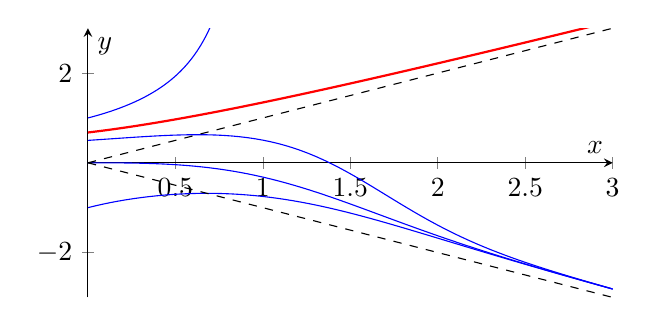
\begin{tikzpicture}\begin{axis}[width=.68\textwidth,height=5cm,axis lines=middle,xlabel={$x$},ylabel={$y$},xmin=0,xmax=3,ymin=-3,ymax=3,clip=true]\addplot[blue]coordinates{(0.00000,-1.00000)(0.04348,-0.95836)(0.08696,-0.92021)(0.13043,-0.88531)(0.17391,-0.85348)(0.21739,-0.82456)(0.26087,-0.79843)(0.30435,-0.77502)(0.34783,-0.75424)(0.39130,-0.73606)(0.43478,-0.72043)(0.47826,-0.70736)(0.52174,-0.69681)(0.56522,-0.68881)(0.60870,-0.68334)(0.65217,-0.68042)(0.69565,-0.68007)(0.73913,-0.68229)(0.78261,-0.68710)(0.82609,-0.69450)(0.86957,-0.70450)(0.91304,-0.71709)(0.95652,-0.73227)(1.00000,-0.75002)(1.04348,-0.77030)(1.08696,-0.79309)(1.13043,-0.81832)(1.17391,-0.84595)(1.21739,-0.87590)(1.26087,-0.90808)(1.30435,-0.94240)(1.34783,-0.97876)(1.39130,-1.01703)(1.43478,-1.05710)(1.47826,-1.09883)(1.52174,-1.14208)(1.56522,-1.18672)(1.60870,-1.23261)(1.65217,-1.27959)(1.69565,-1.32754)(1.73913,-1.37632)(1.78261,-1.42579)(1.82609,-1.47583)(1.86957,-1.52632)(1.91304,-1.57715)(1.95652,-1.62823)(2.00000,-1.67946)(2.04348,-1.73076)(2.08696,-1.78207)(2.13043,-1.83332)(2.17391,-1.88446)(2.21739,-1.93545)(2.26087,-1.98626)(2.30435,-2.03686)(2.34783,-2.08723)(2.39130,-2.13736)(2.43478,-2.18723)(2.47826,-2.23685)(2.52174,-2.28621)(2.56522,-2.33532)(2.60870,-2.38418)(2.65217,-2.43280)(2.69565,-2.48119)(2.73913,-2.52935)(2.78261,-2.57730)(2.82609,-2.62504)(2.86957,-2.67260)(2.91304,-2.71997)(2.95652,-2.76717)(3.00000,-2.81422)};\addplot[blue]coordinates{(0.00000,0.00000)(0.04348,-0.00003)(0.08696,-0.00022)(0.13043,-0.00074)(0.17391,-0.00175)(0.21739,-0.00342)(0.26087,-0.00592)(0.30435,-0.00939)(0.34783,-0.01402)(0.39130,-0.01995)(0.43478,-0.02735)(0.47826,-0.03637)(0.52174,-0.04717)(0.56522,-0.05990)(0.60870,-0.07469)(0.65217,-0.09168)(0.69565,-0.11098)(0.73913,-0.13272)(0.78261,-0.15699)(0.82609,-0.18386)(0.86957,-0.21340)(0.91304,-0.24566)(0.95652,-0.28065)(1.00000,-0.31837)(1.04348,-0.35878)(1.08696,-0.40183)(1.13043,-0.44744)(1.17391,-0.49550)(1.21739,-0.54588)(1.26087,-0.59841)(1.30435,-0.65292)(1.34783,-0.70921)(1.39130,-0.76708)(1.43478,-0.82630)(1.47826,-0.88664)(1.52174,-0.94788)(1.56522,-1.00980)(1.60870,-1.07218)(1.65217,-1.13481)(1.69565,-1.19750)(1.73913,-1.26008)(1.78261,-1.32239)(1.82609,-1.38430)(1.86957,-1.44569)(1.91304,-1.50646)(1.95652,-1.56656)(2.00000,-1.62592)(2.04348,-1.68450)(2.08696,-1.74228)(2.13043,-1.79927)(2.17391,-1.85545)(2.21739,-1.91086)(2.26087,-1.96550)(2.30435,-2.01942)(2.34783,-2.07264)(2.39130,-2.12521)(2.43478,-2.17716)(2.47826,-2.22854)(2.52174,-2.27938)(2.56522,-2.32973)(2.60870,-2.37963)(2.65217,-2.42911)(2.69565,-2.47820)(2.73913,-2.52695)(2.78261,-2.57537)(2.82609,-2.62351)(2.86957,-2.67138)(2.91304,-2.71901)(2.95652,-2.76641)(3.00000,-2.81362)};\addplot[blue]coordinates{(0.00000,0.50000)(0.04348,0.51108)(0.08696,0.52250)(0.13043,0.53412)(0.17391,0.54578)(0.21739,0.55734)(0.26087,0.56863)(0.30435,0.57948)(0.34783,0.58971)(0.39130,0.59913)(0.43478,0.60754)(0.47826,0.61471)(0.52174,0.62043)(0.56522,0.62443)(0.60870,0.62646)(0.65217,0.62624)(0.69565,0.62348)(0.73913,0.61786)(0.78261,0.60906)(0.82609,0.59674)(0.86957,0.58057)(0.91304,0.56019)(0.95652,0.53525)(1.00000,0.50543)(1.04348,0.47041)(1.08696,0.42990)(1.13043,0.38367)(1.17391,0.33153)(1.21739,0.27337)(1.26087,0.20916)(1.30435,0.13897)(1.34783,0.06298)(1.39130,-0.01853)(1.43478,-0.10516)(1.47826,-0.19639)(1.52174,-0.29161)(1.56522,-0.39012)(1.60870,-0.49115)(1.65217,-0.59391)(1.69565,-0.69757)(1.73913,-0.80135)(1.78261,-0.90450)(1.82609,-1.00632)(1.86957,-1.10622)(1.91304,-1.20369)(1.95652,-1.29835)(2.00000,-1.38990)(2.04348,-1.47815)(2.08696,-1.56300)(2.13043,-1.64445)(2.17391,-1.72256)(2.21739,-1.79743)(2.26087,-1.86923)(2.30435,-1.93815)(2.34783,-2.00440)(2.39130,-2.06820)(2.43478,-2.12977)(2.47826,-2.18933)(2.52174,-2.24711)(2.56522,-2.30328)(2.60870,-2.35805)(2.65217,-2.41159)(2.69565,-2.46404)(2.73913,-2.51555)(2.78261,-2.56624)(2.82609,-2.61622)(2.86957,-2.66559)(2.91304,-2.71442)(2.95652,-2.76280)(3.00000,-2.81079)};\addplot[blue]coordinates{(0.00000,1.00000)(0.01041,1.01052)(0.02082,1.02126)(0.03123,1.03222)(0.04164,1.04342)(0.05205,1.05485)(0.06245,1.06653)(0.07286,1.07846)(0.08327,1.09063)(0.09368,1.10308)(0.10409,1.11579)(0.11450,1.12877)(0.12491,1.14204)(0.13532,1.15560)(0.14573,1.16946)(0.15614,1.18363)(0.16654,1.19812)(0.17695,1.21294)(0.18736,1.22810)(0.19777,1.24362)(0.20818,1.25949)(0.21859,1.27574)(0.22900,1.29238)(0.23941,1.30943)(0.24982,1.32689)(0.26023,1.34479)(0.27063,1.36313)(0.28104,1.38195)(0.29145,1.40125)(0.30186,1.42106)(0.31227,1.44140)(0.32268,1.46229)(0.33309,1.48376)(0.34350,1.50583)(0.35391,1.52852)(0.36432,1.55187)(0.37472,1.57590)(0.38513,1.60066)(0.39554,1.62616)(0.40595,1.65246)(0.41636,1.67959)(0.42677,1.70760)(0.43718,1.73652)(0.44759,1.76641)(0.45800,1.79732)(0.46841,1.82931)(0.47881,1.86244)(0.48922,1.89678)(0.49963,1.93238)(0.51004,1.96934)(0.52045,2.00773)(0.53086,2.04765)(0.54127,2.08919)(0.55168,2.13245)(0.56209,2.17756)(0.57250,2.22463)(0.58291,2.27381)(0.59331,2.32525)(0.60372,2.37910)(0.61413,2.43556)(0.62454,2.49481)(0.63495,2.55709)(0.64536,2.62262)(0.65577,2.69170)(0.66618,2.76461)(0.67659,2.84169)(0.68700,2.92332)(0.69740,3.00992)(0.70781,3.10197)(0.71822,3.20000)};\addplot[red,thick]coordinates{(0.00000,0.67598)(0.04348,0.69642)(0.08696,0.71797)(0.13043,0.74057)(0.17391,0.76416)(0.21739,0.78870)(0.26087,0.81413)(0.30435,0.84040)(0.34783,0.86747)(0.39130,0.89530)(0.43478,0.92384)(0.47826,0.95307)(0.52174,0.98293)(0.56522,1.01340)(0.60870,1.04444)(0.65217,1.07603)(0.69565,1.10813)(0.73913,1.14071)(0.78261,1.17376)(0.82609,1.20725)(0.86957,1.24115)(0.91304,1.27544)(0.95652,1.31011)(1.00000,1.34513)(1.04348,1.38048)(1.08696,1.41616)(1.13043,1.45213)(1.17391,1.48840)(1.21739,1.52493)(1.26087,1.56173)(1.30435,1.59877)(1.34783,1.63605)(1.39130,1.67356)(1.43478,1.71127)(1.47826,1.74919)(1.52174,1.78731)(1.56522,1.82561)(1.60870,1.86408)(1.65217,1.90272)(1.69565,1.94153)(1.73913,1.98049)(1.78261,2.01959)(1.82609,2.05884)(1.86957,2.09822)(1.91304,2.13773)(1.95652,2.17736)(2.00000,2.21711)(2.04348,2.25697)(2.08696,2.29694)(2.13043,2.33702)(2.17391,2.37719)(2.21739,2.41746)(2.26087,2.45782)(2.30435,2.49827)(2.34783,2.53881)(2.39130,2.57943)(2.43478,2.62012)(2.47826,2.66089)(2.52174,2.70174)(2.56522,2.74265)(2.60870,2.78363)(2.65217,2.82468)(2.69565,2.86579)(2.73913,2.90696)(2.78261,2.94818)(2.82609,2.98947)(2.86957,3.03080)(2.91304,3.07219)(2.95652,3.11363)(3.00000,3.15512)};\addplot[dashed,domain=0:3]{x};\addplot[dashed,domain=0:3]{-x};\end{axis}\end{tikzpicture}\end{center}
\par\noindent{\small 依据：官方译审并补证（AI辅助）。}
\end{solution}

\begin{exercise}\label{cw:rec02-7}
分界线指一条解曲线：其上、下方的解在 $x$ 增加时有完全不同的命运。画出 $y'=y^2-x^2$ 的分界线，说明两侧的行为。
\end{exercise}
\begin{solution}
代换 $y=-u'/u$ 把方程化为 $u''=x^2u$。为明确分界线，取正函数
\[
 U(x)=\ee^{-x^2/2}\int_0^\infty t^{-1/2}\ee^{-t^2/2-\sqrt2xt}\dd t,\qquad x\ge0.
\]
积分可逐次求导，因为被积函数及其导数有高斯控制。分部积分 $\int_0^\infty (t^{1/2}\ee^{-t^2/2-\sqrt2xt})'\dd t=0$ 给出 $U''=x^2U$。因此 $s=-U'/U$ 是解，且 $s=x+\sqrt2\,\bigl(\int t^{1/2}\ee^{-t^2/2-\sqrt2xt}\dd t\bigr)/\bigl(\int t^{-1/2}\ee^{-t^2/2-\sqrt2xt}\dd t\bigr)>x$。
任意其他解可由降阶写成 $u=U(1+cJ)$，其中 $J(x)=\int_0^xU(v)^{-2}\dd v$。于是
\[
 y=s-\frac{cJ'}{1+cJ},\qquad y(0)-s(0)=-c/U(0)^2.
\]
$J$ 严格增加且无界。上方初值对应 $c<0$，$1+cJ$ 在有限时刻第一次为零，$y\to+\infty$；下方对应 $c>0$，分母始终正，解存在于全部 $x\ge0$，并趋向 $-x$，如下题所证。这正是分界线。示意图用红色表示分界线在右端靠近 $y=x$ 上方；须注意它并不是零斜线 $y=x$。
分界线的红色图在习题\ref{cw:rec02-6}中；在$x=0$，$s(0)=2\Gamma(3/4)/\Gamma(1/4)\approx0.67598$仅用作作图定位，证明不依赖此数值。
\par\noindent{\small 依据：官方译审并补证（AI辅助）；分界存在与两侧行为给出独立解析论证。}
\end{solution}

\begin{exercise}\label{cw:rec02-8}
方程 $y'=y^2-x^2$ 还存在漏斗，多条解在其中互相渐近。用两条等斜线解释，并找出这些解逼近的简单函数（该函数本身不是解）。
\end{exercise}
\begin{solution}
对于 $x>\sqrt{8/3}$，取下界 $L=-x$（等斜率0）和上界 $B=-\sqrt{x^2-2}$（等斜率$-2$）。边界上 $F(x,L)-L'=1>0$，$F(x,B)-B'=-2+x/\sqrt{x^2-2}<0$，故二者夹成不变漏斗，宽度 $x-\sqrt{x^2-2}\to0$，任何在里面的解满足 $y+x\to0$。
还可确认全部分界线以下的解最终进入此带：上一题的积分作 $t=v/(\sqrt2x)$，展开 $\ee^{-v^2/(4x^2)}$ 并以指数衰减控制余项，得
\[
 U=C\ee^{-x^2/2}x^{-1/2}\bigl(1-3/(16x^2)+O(x^{-4})\bigr),\quad
 J=\frac{\ee^{x^2}}{2C^2}\bigl(1+3/(8x^2)+O(x^{-4})\bigr).
\]
同样的展开可逐次求导，故 $s=x+1/(2x)+O(x^{-3})$，$J'/J=2x+O(x^{-3})$。当 $c>0$ 时 $y=-x+1/(2x)+O(x^{-3})$，最终在漏斗内。两解差 $d$ 满足 $d'=(y_1+y_2)d$，因此也趋于0。简单渐近函数是 $-x$；它不是解，因为其导数为$-1$而方程右端为0。官方末句的 $-x+1$ 是笔误，双曲线 $y^2=x^2-1$ 的下支渐近线同样为 $-x$。
\par\noindent{\small 依据：官方译审并补证（AI辅助）；修正官方渐近线并补不变带与渐近推导。}
\end{solution}

\originalsection{第3次习题课：Euler 法与线性模型（2月9日）}
\begin{exercise}\label{cw:rec03-1}
用 Euler 法估计 $y'=y^2-x^2,y(0)=-1$ 的 $y(1.5)$，步长 $h=0.5$。令 $x_{n+1}=x_n+h,y_{n+1}=y_n+m_nh,m_n=F(x_n,y_n)$，列出 $n,x_n,y_n,m_n,m_nh$ 并画折线。
\end{exercise}
\begin{solution}
逐步在旧节点取斜率：
\[\begin{array}{c|rrrr}n&x_n&y_n&m_n&m_nh\\\hline0&0&-1&1&1/2\\1&1/2&-1/2&0&0\\2&1&-1/2&-3/4&-3/8\\3&3/2&-7/8&-&-\end{array}\]
故估计为 $-7/8$。折线连接这四个点。\begin{center}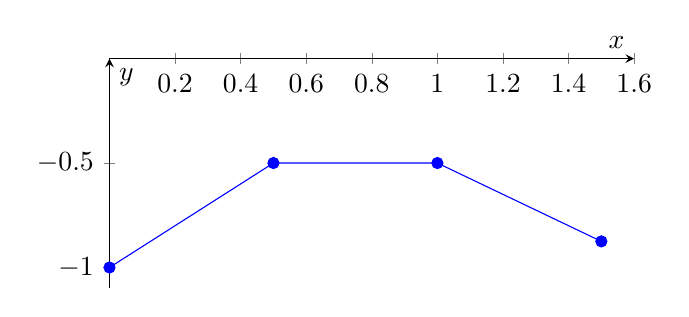
\begin{tikzpicture}\begin{axis}[width=.68\textwidth,height=4.5cm,axis lines=middle,xlabel={$x$},ylabel={$y$},samples=130,xmin=0,xmax=1.6,ymin=-1.1,ymax=0]
\addplot[blue,mark=*] coordinates {(0,-1)(.5,-.5)(1,-.5)(1.5,-.875)};\end{axis}\end{tikzpicture}\end{center}
\par\noindent{\small 依据：官方译审并补证（AI辅助）。}
\end{solution}

\begin{exercise}\label{cw:rec03-2}
上一题的估计偏大还是偏小？
\end{exercise}
\begin{solution}
Euler 折线 $P$ 在三段分别为 $x-1,-1/2,-3x/4+1/4$。其斜率减 $F(x,P)$ 分别为 $2x,x^2-1/4$，以及 $-3/4+7x^2/16+3x/8-1/16$；在各区间均非负，第三式从 $x=1$ 的0递增。所以 $P$ 是上解。从 $d=P-y$ 的方程 $d'=(P+y)d+[P'-F(x,P)]$，积分因子直接给 $d\ge0$（首段内部严格正）。因而 $-7/8$ 偏大；这比仅检查三个点的凹凸性更可靠。
\par\noindent{\small 依据：官方译审并补证（AI辅助）。}
\end{solution}

\begin{exercise}\label{cw:rec03-3}
盐水槽体积为 $V$ 升，浓度 $c$ 克/升的盐水以 $r$ 升/分流入，同速流出，搅拌均匀。以 $x(t)$ 表示槽中盐的克数，写出方程并检查单位、化为标准线性形式。
\end{exercise}
\begin{solution}
流入盐量每分钟 $rc$ 克，流出浓度为 $x/V$，故 $\dot x=rc-rx/V$，即 $\dot x+(r/V)x=rc$。两端单位均为克/分；$V$ 恒定是因为进出体积速率相同。
\par\noindent{\small 依据：官方译审并补证（AI辅助）。}
\end{solution}

\begin{exercise}\label{cw:rec03-4}
设 $c,r$ 恒定，$V=1$ 升、$r=2$ 升/分，$x(0)=0$。求解、长期盐量及达到其一半的时间，并说明物理意义。
\end{exercise}
\begin{solution}
$\dot x+2x=2c$，积分因子 $\ee^{2t}$ 给 $x=c(1-\ee^{-2t})$ 克，其中体积1升已代入。极限为 $c$ 克，相应浓度与输入相同。若 $c>0$，半量时 $\ee^{-2t}=1/2$，即 $t=\log2/2$ 分。
\par\noindent{\small 依据：官方译审并补证（AI辅助）。}
\end{solution}

\begin{exercise}\label{cw:rec03-5}
第一槽的流出液进入另一体积1升且同速流出的均匀搅拌槽；第二槽在 $t=1$ 时无盐。建立第二槽盐量随时间的微分方程。
\end{exercise}
\begin{solution}
以 $z(t)$ 表示第二槽盐量，输入浓度为 $x(t)/1$，所以 $\dot z+2z=2c(1-\ee^{-2t})$，$z(1)=0$，$t\ge1$。保留原题初始时刻1；若进一步积分，$z=c-2ct\ee^{-2t}+c(2-\ee^2)\ee^{-2t}$，代入 $t=1$ 确为0。
\par\noindent{\small 依据：官方译审并补证（AI辅助）。}
\end{solution}

\begin{exercise}\label{cw:rec03-6}
画出电压源、电阻、电容串联电路，取顺时针电流 $I(t)$，源电压 $V(t)$，电阻 $R>0$、电容 $C>0$，满足 $R\dot I+C^{-1}I=\dot V$。当 $V(t)=V_0$ 恒定时，按给定 $I(0)$ 求解，并写作 $c\ee^{-t/\tau}$，求 $c,\tau,I(t+\tau)$。
\end{exercise}
\begin{solution}
$\dot V=0$，故 $\dot I=-I/(RC)$，积分得 $I(t)=I(0)\ee^{-t/(RC)}$。因此 $c=I(0),\tau=RC$（时间单位），且 $I(t+\tau)=I(t)/\ee$。以下示意图中框为电阻、双短线为电容、圆形为电压源。\begin{center}\begin{tikzpicture}[scale=.8]\draw(0,0)--(0,1.3) (0,2.1)--(0,3)--(1.3,3) (2.3,3)--(4,3)--(4,1.9) (4,1.6)--(4,0)--(0,0);\draw (0,1.7) circle(.4);\node at(0,1.7){$V$};\draw(1.3,2.8) rectangle(2.3,3.2);\node at(1.8,3.5){电阻 $R$};\draw(3.6,1.9)--(4.4,1.9) (3.6,1.6)--(4.4,1.6);\node[right]at(4.4,1.75){电容 $C$};\draw[->](2.4,.6)--(1.4,.6) node[midway,above]{$I$};\end{tikzpicture}\end{center}
\par\noindent{\small 依据：官方译审并补证（AI辅助）。}
\end{solution}

\originalsection{第4次习题课：一阶线性方程与积分因子（2月11日）}
\begin{exercise}\label{cw:rec04-1}
Cape Cod 盐池经窄水道连海，池面在短时间的变化与海池水位差及时间长度成正比。同一零点测海面 $y(t)$、池面 $x(t)$。
\begin{enumerate}[label=(\alph*)]\item 建立方程；说明系统、代表系统的算子、输入和输出。\item 高潮恰每 $4\pi$ 小时一次，$y=\cos(\omega t)$，长度用米、时间用小时，求 $\omega$。\item 用积分因子求解，可用 $\int\ee^{kt}\cos\omega t\dd t=\ee^{kt}(k\cos\omega t+\omega\sin\omega t)/(k^2+\omega^2)+C$。\item 另设 $x_p=a\cos\omega t+b\sin\omega t$ 求同一周期解。\end{enumerate}
\end{exercise}
\begin{solution}
(a) $\dot x=k(y-x)$，$k>0$，故 $(D+k)x=ky$。系统是盐池与水道，固定算子为 $D+k$，海面 $y$ 为输入，池面 $x$ 为输出，输入系数为$k$。
(b) $2\pi/\omega=4\pi$，故 $\omega=1/2$ 小时$^{-1}$。
(c) 乘 $\ee^{kt}$ 并积分得
\[x=\frac{k^2\cos\omega t+k\omega\sin\omega t}{k^2+\omega^2}+C\ee^{-kt}.
\]
(d) 比较余弦、正弦系数得到 $ka+\omega b=k$、$kb-\omega a=0$，解得 $a=k^2/(k^2+\omega^2),b=k\omega/(k^2+\omega^2)$，与(c)一致。$k=0$ 时池面恒定，不能从周期强迫确定其常值。
\par\noindent{\small 依据：官方译审并补证（AI辅助）。}
\end{solution}

\begin{exercise}\label{cw:rec04-2}
用解析方法求 $y'=x-2y$ 通解；核对第2次的直线解，画几条解，判断漏斗，并求 $y(0)=1$ 的解。
\end{exercise}
\begin{solution}
乘 $\ee^{2x}$ 得 $(\ee^{2x}y)'=x\ee^{2x}$；积分得 $y=x/2-1/4+C\ee^{-2x}$。$C=0$ 给直线解，任意窄的两条平行线最终夹住所有有限初值解。$y(0)=1$ 给 $C=5/4$，故 $y=x/2-1/4+5\ee^{-2x}/4$。图为同一方程，沿用习题\ref{cw:rec02-1} 的同册图；漏斗的边界方向论证见习题\ref{cw:rec02-4}。
\par\noindent{\small 依据：官方译审并补证（AI辅助）；同一方程方向图回指第2次，积分推导独立列出。}
\end{solution}

\begin{exercise}\label{cw:rec04-3}
把左侧识别为乘积导数，求 $x^2y'+2xy=\sin(2x)$ 通解。
\end{exercise}
\begin{solution}
左侧为 $(x^2y)'$，故 $x^2y=-\cos(2x)/2+C$。在不含0的区间 $y=[C-\cos(2x)/2]/x^2$。若要连续延至0，必须 $C=1/2$；这时 $y=\sin^2x/x^2$，可取 $y(0)=1$，且光滑延拓在0亦满足原式。任意常数公式不能直接在0相除。
\par\noindent{\small 依据：官方译审并补证（AI辅助）。}
\end{solution}

\originalsection{第5次习题课：复数、复指数与相位（2月18日）}
\begin{exercise}\label{cw:rec05-1}
在复平面标出 $z=1+\sqrt3\ii$，求极坐标；再标 $z^n,n=1,2,3,4$，分别写为 $a+b\ii$ 与 $A\ee^{\ii\theta}$，并标 $n=0,-1,-2,-3,-4$ 的点。
\end{exercise}
\begin{solution}
$z=2\ee^{\ii\pi/3}$，所以 $z^n=2^n\ee^{\ii n\pi/3}$。直角坐标依次为
\[\begin{array}{c|ccccc}n&0&1&2&3&4\\\hline z^n&1&1+\sqrt3\ii&-2+2\sqrt3\ii&-8&-8-8\sqrt3\ii\end{array}\]
\[z^{-1}=(1-\sqrt3\ii)/4,\quad z^{-2}=(-1-\sqrt3\ii)/8,\quad z^{-3}=-1/8,\quad z^{-4}=(-1+\sqrt3\ii)/32.\]
特别是 $z^{-4}$ 在上半平面，不能把负幂一概说成在下半平面。下图以两种尺度分别标正幂和非正幂。\begin{center}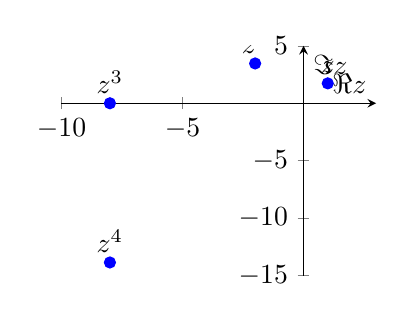
\begin{tikzpicture}\begin{axis}[width=.46\textwidth,height=4.5cm,axis lines=middle,xlabel={$\Re z$},ylabel={$\Im z$},xmin=-10,xmax=3,ymin=-15,ymax=5]\addplot[only marks,blue]coordinates{(1,1.732)(-2,3.464)(-8,0)(-8,-13.856)};\node at(axis cs:1,1.732)[above]{$z$};\node at(axis cs:-2,3.464)[above]{$z^2$};\node at(axis cs:-8,0)[above]{$z^3$};\node at(axis cs:-8,-13.856)[above]{$z^4$};\end{axis}\end{tikzpicture}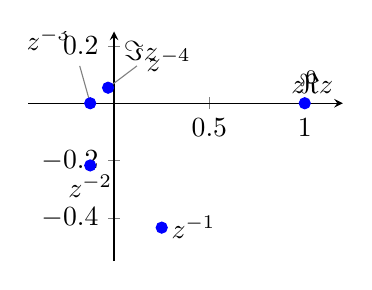
\begin{tikzpicture}\begin{axis}[width=.46\textwidth,height=4.5cm,axis lines=middle,xlabel={$\Re z$},ylabel={$\Im z$},xmin=-.45,xmax=1.2,ymin=-.55,ymax=.25]\addplot[only marks,blue]coordinates{(1,0)(.25,-.433)(-.125,-.2165)(-.125,0)(-.03125,.0541)};\node at(axis cs:1,0)[above]{$z^0$};\node at(axis cs:.25,-.433)[right]{$z^{-1}$};\node at(axis cs:-.125,-.2165)[below]{$z^{-2}$};\node at(axis cs:-.18,.15)[above left]{$z^{-3}$};\draw[gray](axis cs:-.18,.13)--(axis cs:-.125,0);\node at(axis cs:.12,.15)[right]{$z^{-4}$};\draw[gray](axis cs:.12,.13)--(axis cs:-.03125,.0541);\end{axis}\end{tikzpicture}\end{center}
\par\noindent{\small 依据：官方译审并补证（AI辅助）。}
\end{solution}

\begin{exercise}\label{cw:rec05-2}
找出所有满足 $\ee^{a+b\ii}=1+\sqrt3\ii$ 的复数；取最小正 $b$ 后求 $\ee^{n(a+b\ii)}$，$n=1,2,3,4,0,-1,-2,-3,-4$。
\end{exercise}
\begin{solution}
比较模与辐角得 $a=\log2,b=\pi/3+2j\pi,j\in\mathbb Z$。最小正 $b$ 是 $\pi/3$。所有整数 $n$ 均有 $\ee^{n(a+b\ii)}=(\ee^{a+b\ii})^n=z^n$，所以各值、极形式及点位正是习题\ref{cw:rec05-1} 完整列出的九个值。
\par\noindent{\small 依据：官方译审并补证（AI辅助）；九个完全相同的数值回指上题，复对数分支另行推导。}
\end{solution}

\begin{exercise}\label{cw:rec05-3}
各式化为 $A\cos(\omega t-\phi)$，先画以余弦、正弦系数 $a,b$ 为直角边的三角形：
(a) $\cos2t+\sin2t$；(b) $\cos\pi t-\sqrt3\sin\pi t$；(c) $\Re[\ee^{\ii t}/(2+2\ii)]$。
\end{exercise}
\begin{solution}
展开 $A\cos(\omega t-\phi)=A\cos\phi\cos\omega t+A\sin\phi\sin\omega t$，故 $A=\sqrt{a^2+b^2}$，$\phi=\arg(a+b\ii)$。
(a) $(a,b)=(1,1)$，得 $\sqrt2\cos(2t-\pi/4)$；(b) $(1,-\sqrt3)$，得 $2\cos(\pi t+\pi/3)$；(c) $(2+2\ii)^{-1}=(1-\ii)/4$，实部为 $(\cos t+\sin t)/4$，得 $\sqrt2\cos(t-\pi/4)/4$。
三角形中的有向竖边决定相位正负，长度仍取绝对值。\begin{center}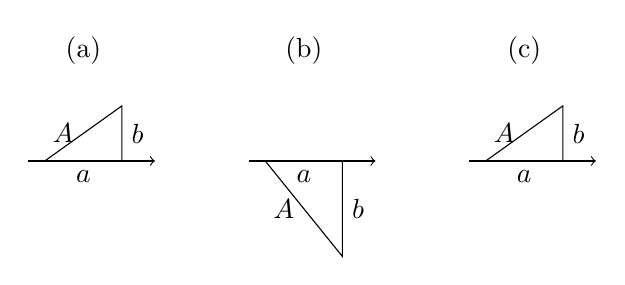
\begin{tikzpicture}[scale=.7]\foreach \p/\a/\b/\lab in {0/1/1/(a),4/1/-1.732/(b),8/1/1/(c)}{\begin{scope}[xshift=\p cm]\draw[->](-.3,0)--(2,0);\draw(0,0)--(1.4,0)--(1.4,\b)--cycle;\node[below]at(.7,0){$a$};\node[right]at(1.4,\b/2){$b$};\node[left]at(.7,\b/2){$A$};\node at(.7,2){\lab};\end{scope}}\end{tikzpicture}\end{center}
\par\noindent{\small 依据：官方译审并补证（AI辅助）。}
\end{solution}

\begin{exercise}\label{cw:rec05-4}
以 $w\ee^t$ 形式求 $\dot x+2x=\ee^t$ 的特解；同样求 $\dot z+2z=\ee^{2\ii t}$，并给两个方程的通解。
\end{exercise}
\begin{solution}
第一式代入得 $3w=1$，故 $x=\ee^t/3+C\ee^{-2t}$。第二式设 $z=w\ee^{2\ii t}$ 得 $(2+2\ii)w=1$，故 $z=\ee^{2\ii t}/(2+2\ii)+C\ee^{-2t}$；此处 $C$ 可以是复数。每个齐次差满足 $\dot h+2h=0$，所以没有遗漏。
\par\noindent{\small 依据：官方译审并补证（AI辅助）。}
\end{solution}

\begin{exercise}\label{cw:rec05-5}
用复替代求 $\dot x+2x=\cos2t$ 的解，再由同一计算得到正弦输入的解。
\end{exercise}
\begin{solution}
求解 $\dot z+2z=\ee^{2\ii t}$ 得 $z_p=(1-\ii)\ee^{2\ii t}/4$。由于算子实系数，实部、虚部分别满足余弦、正弦强迫。因此 $x_{p,\cos}=(\cos2t+\sin2t)/4$，$x_{p,\sin}=(\sin2t-\cos2t)/4$；两者分别加 $C\ee^{-2t}$ 得通解。
\par\noindent{\small 依据：官方译审并补证（AI辅助）。}
\end{solution}

\originalchapter{习题课：二阶方程、共振与 Fourier 响应}
\originalsection{第7次习题课：二阶方程的解（2月25日）}
\begin{exercise}\label{cw:rec07-1}
核验 $x=\cos\omega t$ 与 $x=\sin\omega t$ 都满足谐振子方程 $\ddot x+\omega^2x=0$。
\end{exercise}
\begin{solution}
余弦的二阶导数为 $-\omega^2\cos\omega t$，正弦的二阶导数为 $-\omega^2\sin\omega t$，代入各自抵消。
\par\noindent{\small 依据：官方译审并补证（AI辅助）。}
\end{solution}

\begin{exercise}\label{cw:rec07-2}
进一步核验一般正弦波 $x=A\cos(\omega t-\phi)$ 满足同一方程。
\end{exercise}
\begin{solution}
两次链式求导得 $\ddot x=-A\omega^2\cos(\omega t-\phi)=-\omega^2x$。振幅、相位任意不改变结论。
\par\noindent{\small 依据：官方译审并补证（AI辅助）。}
\end{solution}

\begin{exercise}\label{cw:rec07-3}
哪些 $x=A\cos(\omega t-\phi)$ 满足 $x(0)=0$？这是否违反微分方程的唯一性定理？
\end{exercise}
\begin{solution}
$A\cos\phi=0$。除零解外，$\phi=\pi/2+j\pi$，相应解为任意倍数的 $\sin\omega t$。二阶方程的唯一性需要同时指定位置和速度；只给位置不能唯一决定解。化为 $(x,v)'=(v,-\omega^2x)$ 后，一阶系统的两个初值也表明此点。
\par\noindent{\small 依据：官方译审并补证（AI辅助）。}
\end{solution}

\begin{exercise}\label{cw:rec07-4}
给定 $x_0,\dot x_0$，求 $\ddot x+\omega^2x=0$ 满足 $x(0)=x_0,\dot x(0)=\dot x_0$ 的解，有多少个？
\end{exercise}
\begin{solution}
$\omega\ne0$ 时 $x=x_0\cos\omega t+(\dot x_0/\omega)\sin\omega t$，其两个初值直接成立。差解的能量 $v^2+\omega^2x^2$ 恒定，零初值使能量恒为0，故解唯一。$\omega=0$ 时唯一解为 $x=x_0+\dot x_0t$。
\par\noindent{\small 依据：官方译审并补证（AI辅助）。}
\end{solution}

\begin{exercise}\label{cw:rec07-5}
若复数常数 $r$ 使 $\ee^{rt}$ 满足 $\ddot x+kx=0$，$r$ 必须为何值？
\end{exercise}
\begin{solution}
代入得 $(r^2+k)\ee^{rt}=0$，指数不为0，故 $r^2=-k$。$k>0$ 时 $r=\pm\ii\sqrt k$，$k=0$ 时 $r=0$，$k<0$ 时 $r=\pm\sqrt{-k}$。
\par\noindent{\small 依据：官方译审并补证（AI辅助）。}
\end{solution}

\begin{exercise}\label{cw:rec07-6}
对 $\ddot x-a^2x=0$ 求规范化解 $x_1(0)=1,\dot x_1(0)=0$ 及 $x_2(0)=0,\dot x_2(0)=1$。
\end{exercise}
\begin{solution}
$a\ne0$ 时从 $x=c_1\ee^{at}+c_2\ee^{-at}$ 比较初值得 $x_1=\cosh at$，$x_2=\sinh(at)/a$。二阶导数与初值逐一满足要求。$a=0$ 时分别为1、$t$，也是这两个公式的连续极限。
\par\noindent{\small 依据：官方译审并补证（AI辅助）。}
\end{solution}

\originalsection{第8次习题课：二阶常系数齐次方程（3月2日）}
\begin{exercise}\label{cw:rec08-1}
对 $\ddot x+\omega^2x=0$ 求特征多项式、根、指数解及其实部与虚部。
\end{exercise}
\begin{solution}
$p(s)=s^2+\omega^2$，根为 $\pm\ii\omega$，指数解为 $\ee^{\pm\ii\omega t}$，实部均为 $\cos\omega t$，虚部为 $\pm\sin\omega t$。$\omega\ne0$ 时后二者构成实基本解；$\omega=0$ 时须补重根解$t$。
\par\noindent{\small 依据：官方译审并补证（AI辅助）。}
\end{solution}

\begin{exercise}\label{cw:rec08-2}
已知 $\ee^{-t/2}\cos3t$ 是 $m\ddot x+b\dot x+kx=0$ 的解，$m,b,k$ 为实数、$m\ne0$。
(a) 确定它们的关系；(b) 写一个指数解；(c) 画指数解在复平面的轨迹及实部时间图，说明关系；(d) 给通解。
\end{exercise}
\begin{solution}
(a) 实部求导并比较独立的正余弦项，等价于特征根 $-1/2\pm3\ii$；因此 $p(s)=m[(s+1/2)^2+9]$，$b=m,k=37m/4$。
(b) $z=\ee^{(-1/2+3\ii)t}$。
(c) $|z|=\ee^{-t/2},\arg z=3t$，故逆时针向内螺旋；实部是这个轨迹在实轴上的投影，并按时间展开。
(d) $x=\ee^{-t/2}(C_1\cos3t+C_2\sin3t)$，两解初值矩阵行列式为3，保证独立。\begin{center}\begin{tikzpicture}\begin{axis}[width=.44\textwidth,height=4.2cm,axis lines=middle,xlabel={实部},ylabel={虚部},xmin=-1,xmax=1,ymin=-1,ymax=1]\addplot[blue,domain=0:10,samples=230]({exp(-x/2)*cos(deg(3*x))},{exp(-x/2)*sin(deg(3*x))});\end{axis}\end{tikzpicture}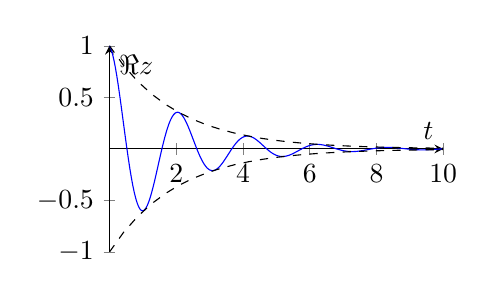
\begin{tikzpicture}\begin{axis}[width=.48\textwidth,height=4.2cm,axis lines=middle,xlabel={$t$},ylabel={$\Re z$},xmin=0,xmax=10,ymin=-1,ymax=1]\addplot[blue,domain=0:10,samples=230]{exp(-x/2)*cos(deg(3*x))};\addplot[dashed,domain=0:10]{exp(-x/2)};\addplot[dashed,domain=0:10]{-exp(-x/2)};\end{axis}\end{tikzpicture}\end{center}
\par\noindent{\small 依据：官方译审并补证（AI辅助）。}
\end{solution}

\begin{exercise}\label{cw:rec08-3}
阻尼正弦 $x=A\ee^{-at}\cos\omega t$ 的伪周期为 $2\pi/\omega$，相邻零点距离为其一半。相邻极大值点间距是否固定？是多少？
\end{exercise}
\begin{solution}
取 $A\ne0,\omega>0$。$\dot x=-A\ee^{-at}(a\cos\omega t+\omega\sin\omega t)$，驻点满足 $\tan\omega t=-a/\omega$，间距 $\pi/\omega$。驻点处 $\ddot x=-(a^2+\omega^2)x$，正峰为极大、负峰为极小，交替出现，因此相邻极大值相隔 $2\pi/\omega$，恒定。零函数或 $\omega=0$ 没有这类相邻波峰。
\par\noindent{\small 依据：官方译审并补证（AI辅助）。}
\end{solution}

\begin{exercise}\label{cw:rec08-4}
相邻极大值时刻为 $t_0,t_1$，求 $x(t_1)/x(t_0)$；能否由图估计 $a$？
\end{exercise}
\begin{solution}
上一题给 $\omega(t_1-t_0)=2\pi$，余弦因子相同，故比值为 $\ee^{-a(t_1-t_0)}$。于是 $a=\log[x(t_0)/x(t_1)]/(t_1-t_0)$，两个正峰的高度与间距即可确定衰减率。
\par\noindent{\small 依据：官方译审并补证（AI辅助）。}
\end{solution}

\begin{exercise}\label{cw:rec08-5}
何值的 $b$ 使 $\ddot x+b\dot x+x=0$ 临界阻尼？求规范化解 $x_1(0)=1,\dot x_1(0)=0$ 与 $x_2(0)=0,\dot x_2(0)=1$；再求 $x(0)=2,\dot x(0)=3$ 的解。
\end{exercise}
\begin{solution}
判别式 $b^2-4=0$ 给 $b=\pm2$；阻尼要求 $b>0$，故取2。通解 $(c_0+c_1t)\ee^{-t}$，初值为 $(c_0,c_1-c_0)$。因此 $x_1=(1+t)\ee^{-t}$、$x_2=t\ee^{-t}$，最后一解 $2x_1+3x_2=(2+5t)\ee^{-t}$。$b=-2$ 为重正根导致增长，不是临界阻尼。
\par\noindent{\small 依据：官方译审并补证（AI辅助）。}
\end{solution}

\originalsection{第9次习题课：指数与正弦输入（3月4日）}
\begin{exercise}\label{cw:rec09-1}
求 $A$ 使 $A\sin3t$ 满足 $\ddot x+4x=\sin3t$，并求通解。
\end{exercise}
\begin{solution}
代入左侧为 $(4-9)A\sin3t$，所以 $A=-1/5$。齐次根为 $\pm2\ii$，故 $x=-\sin3t/5+C_1\cos2t+C_2\sin2t$。
\par\noindent{\small 依据：官方译审并补证（AI辅助）。}
\end{solution}

\begin{exercise}\label{cw:rec09-2}
对 $\omega\ge0$ 求 $A$ 使 $A\cos\omega t$ 满足 $\ddot x+4x=\cos\omega t$；分别画 $\omega=0,1,3$ 的输入与响应，再画 $0\le\omega\le5$ 时 $A(\omega)$，说明共振点及正负号的意义。
\end{exercise}
\begin{solution}
$A(4-\omega^2)=1$，所以 $\omega\ne2$ 时 $A=1/(4-\omega^2)$。$\omega=0,1,3$ 时分别为 $1/4,1/3,-1/5$；正号为同相，负号为反相。$\omega=2$ 无此形式特解而发生共振，不能将无限值代作解。下图黑线为输入，蓝线为响应。\begin{center}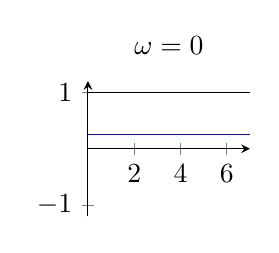
\begin{tikzpicture}\begin{axis}[width=.3\textwidth,height=3.3cm,axis lines=middle,title={$\omega=0$},xmin=0,xmax=7,ymin=-1.2,ymax=1.2]\addplot[black,domain=0:7]{1};\addplot[blue,domain=0:7]{.25};\end{axis}\end{tikzpicture}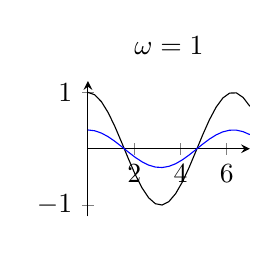
\begin{tikzpicture}\begin{axis}[width=.3\textwidth,height=3.3cm,axis lines=middle,title={$\omega=1$},xmin=0,xmax=7,ymin=-1.2,ymax=1.2]\addplot[black,domain=0:7]{cos(deg(x))};\addplot[blue,domain=0:7]{cos(deg(x))/3};\end{axis}\end{tikzpicture}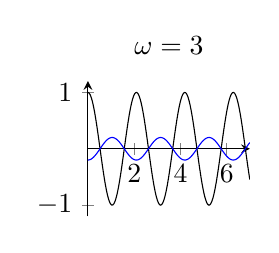
\begin{tikzpicture}\begin{axis}[width=.3\textwidth,height=3.3cm,axis lines=middle,title={$\omega=3$},xmin=0,xmax=7,ymin=-1.2,ymax=1.2]\addplot[black,domain=0:7,samples=150]{cos(deg(3*x))};\addplot[blue,domain=0:7,samples=150]{-cos(deg(3*x))/5};\end{axis}\end{tikzpicture}\end{center}\begin{center}\begin{tikzpicture}\begin{axis}[width=.68\textwidth,height=4.5cm,axis lines=middle,xlabel={$\omega$},ylabel={$A$},samples=130,xmin=0,xmax=5,ymin=-4,ymax=4]
\addplot[blue,domain=0:1.94]{1/(4-x*x)};\addplot[blue,domain=2.06:5]{1/(4-x*x)};\draw[dashed] (axis cs:2,-4)--(axis cs:2,4);\end{axis}\end{tikzpicture}\end{center}
\par\noindent{\small 依据：官方译审并补证（AI辅助）。}
\end{solution}

\begin{exercise}\label{cw:rec09-3}
求 $x^{(4)}-x=\ee^{-2t}$ 的指数型特解。
\end{exercise}
\begin{solution}
设 $x_p=B\ee^{-2t}$，四阶导数为 $16B\ee^{-2t}$，左端为 $15B\ee^{-2t}$，故 $x_p=\ee^{-2t}/15$。
\par\noindent{\small 依据：官方译审并补证（AI辅助）。}
\end{solution}

\begin{exercise}\label{cw:rec09-4}
求 $x^{(4)}-x=\cos2t$ 的正弦型特解。
\end{exercise}
\begin{solution}
余弦的四阶导数为 $16\cos2t$，因此 $x_p=\cos2t/15$ 满足方程。等价地 $p(2\ii)=(2\ii)^4-1=15$，取复指数响应的实部。
\par\noindent{\small 依据：官方译审并补证（AI辅助）。}
\end{solution}

\begin{exercise}\label{cw:rec09-5}
求第3、4题两个四阶非齐次方程的通解。
\end{exercise}
\begin{solution}
$p(s)=s^4-1=(s-1)(s+1)(s^2+1)$，四个互异根给 $x_h=C_1\ee^t+C_2\ee^{-t}+C_3\cos t+C_4\sin t$。分别加第3题 $\ee^{-2t}/15$ 或第4题 $\cos2t/15$ 就是所需通解。相同齐次方程的完整四维解空间在此只写一次。
\par\noindent{\small 依据：官方译审并补证（AI辅助）。}
\end{solution}

\originalsection{第10次习题课：增益、相位滞后与待定系数（3月9日）}
\begin{exercise}\label{cw:rec10-1}
解释指数响应公式（ERF）的记号：$p(D)x=A\ee^{rt}$ 在 $p(r)\ne0$ 时有 $x_p=A\ee^{rt}/p(r)$；若 $p(r)=0,p'(r)\ne0$，则有 $x_p=At\ee^{rt}/p'(r)$。
\end{exercise}
\begin{solution}
$D=\dd/\dd t$ 是微分算子，$p(s)=\sum_{j=0}^na_js^j$ 是常系数算子的多项式，$p(D)=\sum a_jD^j$；$r$ 是可取复值的输入指数，$A$ 是输入系数，$x_p$ 表示特解，$p'(r)$ 是多项式对其变量求导后在$r$的值。因 $D^j\ee^{rt}=r^j\ee^{rt}$，有 $p(D)\ee^{rt}=p(r)\ee^{rt}$，立即得到非共振公式。
对 $r$ 求导（有限和允许交换）得 $p(D)(t\ee^{rt})=p'(r)\ee^{rt}+p(r)t\ee^{rt}$，故在单根共振时得到第二式。多重根需要更高次$t$因子，不能继续除以零。实系数算子可取实部、虚部得到实正弦响应。
\par\noindent{\small 依据：编者补解（AI辅助）；配套官方解答缺第1题。}
\end{solution}

\begin{exercise}\label{cw:rec10-2}
说明由弹簧端驱动的质量--弹簧--阻尼器为何满足 $m\ddot x+b\dot x+kx=ky$。$x$ 为质量块位置，$y$ 为弹簧另一端的位置标记，且 $x=y$ 时弹簧自然放松。
\end{exercise}
\begin{solution}
原题以自然长度调整位置基准，使伸长为 $x-y$。弹簧力 $-k(x-y)$，固定阻尼器力 $-b\dot x$；Newton 方程为 $m\ddot x=-b\dot x-k(x-y)$，移项得到原式。关键是阻尼器相对固定支座，若阻尼器另一端也移动则其力需改写。
\par\noindent{\small 依据：官方译审并补证（AI辅助）。}
\end{solution}

\begin{exercise}\label{cw:rec10-3}
取 $m=1,b=3,k=4,y=A\cos t$，把输入复替代，求稳态指数响应 $z_p=Hy_{\rm cx}$、复增益 $H=|H|\ee^{-\ii\phi}$、增益与相位滞后、稳态实解；质量振幅比驱动端振幅 $A$ 大还是小？
\end{exercise}
\begin{solution}
$y_{\rm cx}=A\ee^{\ii t}$，$p(s)=s^2+3s+4$，$p(\ii)=3+3\ii$。故 $z_p=4A\ee^{\ii t}/(3+3\ii)$，$H=(2/3)(1-\ii)=(2\sqrt2/3)\ee^{-\ii\pi/4}$。增益 $2\sqrt2/3<1$，相位滞后 $\pi/4$，$x_p=(2\sqrt2A/3)\cos(t-\pi/4)$，振幅小于 $A$（按 $A\ge0$ 的振幅约定）。齐次根实部为$-3/2$，所以其他响应的瞬态衰减。
\par\noindent{\small 依据：官方译审并补证（AI辅助）。}
\end{solution}

\begin{exercise}\label{cw:rec10-4}
求 $\ddot x-x=t^2+t+1$ 的多项式解。
\end{exercise}
\begin{solution}
设 $x=at^2+bt+c$，左侧 $-at^2-bt+2a-c$。比较得 $a=-1,b=-1,c=-3$，所以 $x=-t^2-t-3$。若多项式次数更高，最高项在$-x$中无法被二阶导数抵消，故没有另一个多项式解。
\par\noindent{\small 依据：官方译审并补证（AI辅助）。}
\end{solution}

\begin{exercise}\label{cw:rec10-5}
用复替代并尝试 ERF 求 $\ddot x+4x=\cos2t$ 的一个解。
\end{exercise}
\begin{solution}
$p(s)=s^2+4$，$p(2\ii)=0,p'(2\ii)=4\ii$，使用单根共振公式：$z_p=t\ee^{2\ii t}/(4\ii)$。取实部得 $x_p=t\sin2t/4$。直接求导给 $\ddot x_p+4x_p=\cos2t$，体现振幅线性增长。
\par\noindent{\small 依据：官方译审并补证（AI辅助）。}
\end{solution}

\originalsection{第11次习题课：频率响应（3月11日）}
本次系统为直接外力驱动：$\ddot x+\frac14\dot x+2x=F_{\rm ext}$，输入 $F_{\rm ext}=\cos\omega t$（振幅1），稳态响应 $x_p=g(\omega)\cos(\omega t-\phi)$。原题建议用 Amplitude and Phase: Second order, IV；以下均为解析计算。
\begin{exercise}\label{cw:rec11-1}
以 $F_{\rm cx}=\ee^{\ii\omega t}$ 求复增益 $H(\omega)$，使 $z_p=H(\omega)F_{\rm cx}$。
\end{exercise}
\begin{solution}
$p(\ii\omega)=2-\omega^2+\ii\omega/4$，故 $H=(2-\omega^2+\ii\omega/4)^{-1}$。乘共轭可写为 $(2-\omega^2-\ii\omega/4)/[(2-\omega^2)^2+\omega^2/16]$。$\omega\ge0$ 时分母不为0。
\par\noindent{\small 依据：官方译审并补证（AI辅助）。}
\end{solution}

\begin{exercise}\label{cw:rec11-2}
求 $g(\omega)=|H(\omega)|$，以及 $\omega=1$ 的振幅。
\end{exercise}
\begin{solution}
$g=[(2-\omega^2)^2+\omega^2/16]^{-1/2}=[\omega^4-63\omega^2/16+4]^{-1/2}$。所以 $g(1)=4/\sqrt{17}$。因输入振幅为1，响应振幅正是这个数。
\par\noindent{\small 依据：官方译审并补证（AI辅助）。}
\end{solution}

\begin{exercise}\label{cw:rec11-3}
求使振幅最大的共振圆频率 $\omega_r$；可最小化分母的平方。
\end{exercise}
\begin{solution}
令 $z=\omega^2\ge0$，$g^{-2}=z^2-63z/16+4$ 是开口向上抛物线，唯一最小点为 $z=63/32$。故 $\omega_r=\sqrt{63/32}=3\sqrt{14}/8$；这种全局最小论证同时排除端点$\omega=0$。
\par\noindent{\small 依据：官方译审并补证（AI辅助）。}
\end{solution}

\begin{exercise}\label{cw:rec11-4}
在共振频率相位似乎约为 $\pi/2$，它是否恰好等于 $\pi/2$？究竟哪个频率使滞后为四分之一周期？
\end{exercise}
\begin{solution}
相位 $\phi=\arg(2-\omega^2+\ii\omega/4)$ 取 $[0,\pi]$。恰为 $\pi/2$ 要求实部0且虚部正，故 $\omega=\sqrt2$。共振点实部为 $2-63/32=1/32>0$，所以相位略小于$\pi/2$；其正切为 $3\sqrt{14}$，约为$84.91^\circ$。
\par\noindent{\small 依据：官方译审并补证（AI辅助）；补官方未明确给出的精确频率。}
\end{solution}

\begin{exercise}\label{cw:rec11-5}
哪个圆频率使相位滞后为 $\pi/4$？哪个使其为 $3\pi/4$？
\end{exercise}
\begin{solution}
第一种要求 $2-\omega^2=\omega/4>0$，即 $4\omega^2+\omega-8=0$，正根 $\omega=(\sqrt{129}-1)/8$。第二种要求 $2-\omega^2=-\omega/4<0$，正根 $(\sqrt{129}+1)/8$。用象限约束消除仅取正切导致的相位歧义。
\par\noindent{\small 依据：官方译审并补证（AI辅助）。}
\end{solution}

\begin{exercise}\label{cw:rec11-6}
另求 $\ddot x+3\dot x+2x=t\ee^{-t}$ 的一个解。
\end{exercise}
\begin{solution}
令 $x=u\ee^{-t}$，算子平移得左端 $\ee^{-t}(\ddot u+\dot u)$，故需 $\ddot u+\dot u=t$。取 $\dot u=t-1$，积分取 $u=t^2/2-t$，得到 $x_p=(t^2/2-t)\ee^{-t}$。
\par\noindent{\small 依据：官方译审并补证（AI辅助）。}
\end{solution}

\originalsection{第13次习题课：Fourier 级数入门与周期（3月18日）}
\begin{exercise}\label{cw:rec13-1}
迅速写出 $\ddot x+\omega_n^2x=0$ 的通解。
\end{exercise}
\begin{solution}
$\omega_n>0$ 时，特征根为 $\pm\ii\omega_n$，通解 $C_1\cos\omega_nt+C_2\sin\omega_nt$；若允许 $\omega_n=0$，通解为 $C_1+C_2t$。
\par\noindent{\small 依据：官方译审并补证（AI辅助）。}
\end{solution}

\begin{exercise}\label{cw:rec13-2}
解释为什么在 $\omega\ne\pm\omega_n$ 时，$\ddot x+\omega_n^2x=a\cos\omega t$ 和 $\ddot x+\omega_n^2x=b\sin\omega t$ 分别有特解 $a\cos\omega t/(\omega_n^2-\omega^2)$ 与 $b\sin\omega t/(\omega_n^2-\omega^2)$。
\end{exercise}
\begin{solution}
两次微分对正余弦都乘 $-\omega^2$，加 $\omega_n^2$ 后乘 $\omega_n^2-\omega^2$，故除以此非零因子恰还原输入。亦可用 $p(\ii\omega)=\omega_n^2-\omega^2$ 的指数响应公式。
\par\noindent{\small 依据：官方译审并补证（AI辅助）。}
\end{solution}

\begin{exercise}\label{cw:rec13-3}
对 $\ddot x+\omega_n^2x=\cos\omega_nt$ 求特解、通解。是否存在对所有 $t$ 有 $|x(t)|<10^6$ 的解？是否存在周期解？
\end{exercise}
\begin{solution}
$\omega_n>0$ 时共振给 $x_p=t\sin\omega_nt/(2\omega_n)$，通解再加 $C_1\cos\omega_nt+C_2\sin\omega_nt$。取 $t_j=(2j\pi+\pi/2)/\omega_n$，则 $x(t_j)=t_j/(2\omega_n)+C_2\to\infty$。所以没有有界解，也没有连续周期解。$\omega_n=0$ 时方程为 $\ddot x=1$，通解 $t^2/2+C_1+C_2t$，结论仍然相同。
\par\noindent{\small 依据：官方译审并补证（AI辅助）。}
\end{solution}

\begin{exercise}\label{cw:rec13-4}
在同一坐标系画 $\sin t,\sin2t$ 及和 $f(t)=\sin t+\sin2t$。在两项同为0的点求导数，求三个函数的最小周期。
\end{exercise}
\begin{solution}
$f(k\pi)=0$，$f'(k\pi)=(-1)^k+2$，偶数$k$斜率3，奇数$k$斜率1。三个最小周期为 $2\pi,\pi,2\pi$；和式中频率1项非零，不能缩成$\pi$。图中黑虚线为$\sin t$、灰线为$\sin2t$、蓝线为和。\begin{center}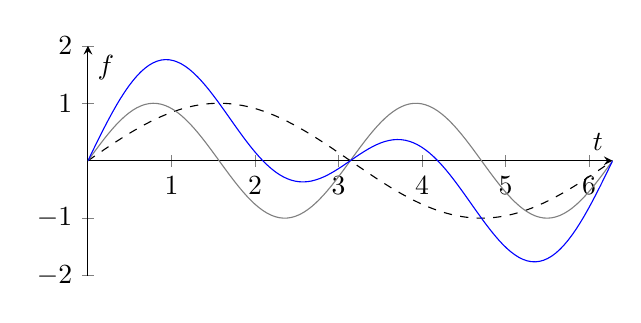
\begin{tikzpicture}\begin{axis}[width=.68\textwidth,height=4.5cm,axis lines=middle,xlabel={$t$},ylabel={$f$},samples=130,xmin=0,xmax=6.283,ymin=-2,ymax=2]
\addplot[black,dashed,domain=0:6.283]{sin(deg(x))};\addplot[gray,domain=0:6.283]{sin(deg(2*x))};\addplot[blue,domain=0:6.283]{sin(deg(x))+sin(deg(2*x))};\end{axis}\end{tikzpicture}\end{center}
\par\noindent{\small 依据：官方译审并补证（AI辅助）。}
\end{solution}

\begin{exercise}\label{cw:rec13-5}
设 $b_1,b_2\ne0$，哪些 $\omega_n$ 使 $\ddot x+\omega_n^2x=b_1\sin t+b_2\sin2t$ 有周期解？若有，举出一个。
\end{exercise}
\begin{solution}
$\omega_n^2\ne1,4$ 时可取 $x_p=b_1\sin t/(\omega_n^2-1)+b_2\sin2t/(\omega_n^2-4)$，周期$2\pi$。若 $\omega_n^2$ 等于1或4，对应非零输入产生 $t\cos\omega_nt$，有界的其他频率项和齐次项不能消除此增长，故无周期解。若约定$\omega_n\ge0$，只排除1、2；允许负值则同时排除$-1,-2$。
\par\noindent{\small 依据：官方译审并补证（AI辅助）。}
\end{solution}

\begin{exercise}\label{cw:rec13-6}
哪些实数 $\omega$ 使 $\sin t+\sin\omega t$ 周期？周期是多少？
\end{exercise}
\begin{solution}
若 $\omega=-1$，和恒为0，每个 $P>0$ 都是周期，没有最小正周期。$\omega=0$ 或1时最小周期为$2\pi$。
当 $\omega\notin\{0,\pm1\}$，函数由四个不同频率 $\pm1,\pm\omega$ 的指数项组成。若有周期$P$，相减 $f(t+P)-f(t)=0$，不同指数函数线性独立（在0求前四阶导数得到非零 Vandermonde 行列式），所以 $\ee^{\ii P}=\ee^{\ii\omega P}=1$。因此 $P=2\pi q$、$\omega P=2\pi p$，$\omega=p/q$ 必须有理。反之，若 $\omega=p/q$ 为既约分数，$q>0$，则 $2\pi q$ 是最小周期，全部周期为其正整数倍。负频率改变符号但不改变可公度条件。
\par\noindent{\small 依据：官方译审并补证（AI辅助）；补频率独立论证与负频率抵消例外。}
\end{solution}

\originalsection{第14次习题课：Fourier 系数与变换（3月30日）}
约定标准方波 $\operatorname{sq}(t)$ 为奇函数，周期$2\pi$，在$0<t<\pi$取1，跳点取左右平均。其级数为 $\frac4\pi\sum_{j\ge0}\sin((2j+1)t)/(2j+1)$。本节函数在跳点同样按中点值理解。
\begin{exercise}\label{cw:rec14-1}
画偶函数 $f$：周期$2\pi$，$0<t<\pi/2$ 时为2，$\pi/2<t<\pi$ 时为0。
(a) 用系数积分求级数，先利用奇偶性；(b) 用标准方波及三角恒等式另求；(c) 求$f-1$的级数。
\end{exercise}
\begin{solution}
(a) 偶性给 $b_n=0$；$a_0=\pi^{-1}\int_{-\pi}^\pi f=2$，$a_n=(4/\pi)\int_0^{\pi/2}\cos nt\dd t=4\sin(n\pi/2)/(n\pi)$。所以
\[f=1+\frac4\pi\sum_{j\ge0}\frac{(-1)^j\cos((2j+1)t)}{2j+1}.\]
(b) $f=1+\operatorname{sq}(t+\pi/2)$，因为平移后的方波正段恰为中心半周期；用 $\sin((2j+1)(t+\pi/2))=(-1)^j\cos((2j+1)t)$ 得同式。
(c) 去常数项1即可。以下图上跳点圆点取中点值1。\begin{center}\begin{tikzpicture}\begin{axis}[width=.68\textwidth,height=4.5cm,axis lines=middle,xlabel={$t$},ylabel={$f$},samples=130,xmin=-3.2,xmax=3.2,ymin=-.2,ymax=2.4]
\addplot[blue]coordinates{(-3.142,0)(-1.571,0)};\addplot[blue]coordinates{(-1.571,2)(1.571,2)};\addplot[blue]coordinates{(1.571,0)(3.142,0)};\addplot[only marks]coordinates{(-1.571,1)(1.571,1)};\end{axis}\end{tikzpicture}\end{center}
\par\noindent{\small 依据：官方译审并补证（AI辅助）。}
\end{solution}

\begin{exercise}\label{cw:rec14-2}
求 $\sin^2t$ 的 Fourier 级数。
\end{exercise}
\begin{solution}
倍角公式 $\sin^2t=(1-\cos2t)/2$ 已是有限 Fourier 级数。按 $a_0/2$ 的 convention，$a_0=1,a_2=-1/2$，其他$a_n,b_n$均为0。
\par\noindent{\small 依据：官方译审并补证（AI辅助）。}
\end{solution}

\begin{exercise}\label{cw:rec14-3}
画奇函数 $g$，周期$\pi$，在 $0<x<\pi/2$ 时为1。$2\pi$亦是其周期；用标准方波求其级数。
\end{exercise}
\begin{solution}
$g(x)=\operatorname{sq}(2x)$，所以 $g=\frac4\pi\sum_{j\ge0}\sin(2(2j+1)x)/(2j+1)$。频率只出现$2,6,10,\ldots$，系数分母仍是$1,3,5,\ldots$。\begin{center}\begin{tikzpicture}\begin{axis}[width=.68\textwidth,height=4.5cm,axis lines=middle,xlabel={$x$},ylabel={$g$},samples=130,xmin=-3.3,xmax=3.3,ymin=-1.3,ymax=1.3]
\addplot[blue] coordinates{(-3.142,1)(-1.571,1)};\addplot[blue]coordinates{(-1.571,-1)(0,-1)};\addplot[blue]coordinates{(0,1)(1.571,1)};\addplot[blue]coordinates{(1.571,-1)(3.142,-1)};\addplot[only marks]coordinates{(-3.142,0)(-1.571,0)(0,0)(1.571,0)(3.142,0)};\end{axis}\end{tikzpicture}\end{center}
\par\noindent{\small 依据：官方译审并补证（AI辅助）。}
\end{solution}

\begin{exercise}\label{cw:rec14-4}
画奇函数 $h$，周期$2\pi$；$0<t<\pi/2$ 时 $h=t$，$\pi/2<t<\pi$ 时 $h=\pi-t$。由第1(c)题求级数。
\end{exercise}
\begin{solution}
$h$ 连续、分段线性，除转角外 $h'=f-1$。对第1(c)题积分，并用$h(0)=0$，得
\[h(t)=\frac4\pi\sum_{j\ge0}\frac{(-1)^j\sin((2j+1)t)}{(2j+1)^2}.\]
积分合法：方波是$L^2$函数，其 Fourier 部分和在$L^2$中收敛，积分误差由 Cauchy--Schwarz 至多为$\sqrt{2\pi}$倍$L^2$误差；所得$1/n^2$级数一致收敛，故处处给出连续的$h$。\begin{center}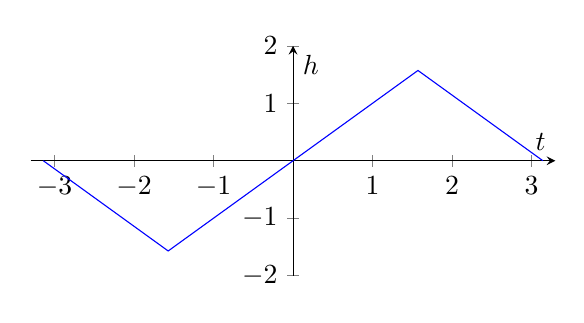
\begin{tikzpicture}\begin{axis}[width=.68\textwidth,height=4.5cm,axis lines=middle,xlabel={$t$},ylabel={$h$},samples=130,xmin=-3.3,xmax=3.3,ymin=-2,ymax=2]
\addplot[blue] coordinates{(-3.142,0)(-1.571,-1.571)(0,0)(1.571,1.571)(3.142,0)};\end{axis}\end{tikzpicture}\end{center}
\par\noindent{\small 依据：官方译审并补证（AI辅助）。}
\end{solution}

\begin{exercise}\label{cw:rec14-5}
解释为什么任意定义在对称区间的函数 $g(x)$ 都唯一分解成偶函数与奇函数之和；求 $\ee^x$ 的两部分。
\end{exercise}
\begin{solution}
$E=[g(x)+g(-x)]/2$ 为偶，$O=[g(x)-g(-x)]/2$ 为奇，且$E+O=g$。若$g=E_1+O_1$，反射给$g(-x)=E_1-O_1$，相加相减强制得到上述两个公式，故唯一。指数函数的两部分是$\cosh x$与$\sinh x$。
\par\noindent{\small 依据：官方译审并补证（AI辅助）。}
\end{solution}

\originalsection{第15次习题课：Fourier 级数与谐波响应（4月1日）}
\begin{exercise}\label{cw:rec15-1}
偶函数 $f$ 周期$2\pi$，在 $-\pi<t<\pi$ 等于 $|t|$，画图。已知
\[f(t)=\frac\pi2-\frac4\pi\sum_{k\ge1,\ k\text{奇}}\frac{\cos kt}{k^2}.\]
把其图形水平缩放至圆频率$\omega>0$，求 $g$ 与$f$的关系及$g$的级数。
\end{exercise}
\begin{solution}
$g(t)=f(\omega t)$，周期变为$2\pi/\omega$，振幅不变。代入得 $g=\pi/2-(4/\pi)\sum_{k\text{奇}}\cos(k\omega t)/k^2$。注意只改变余弦自变量，不能在系数额外引入$\omega^2$。\begin{center}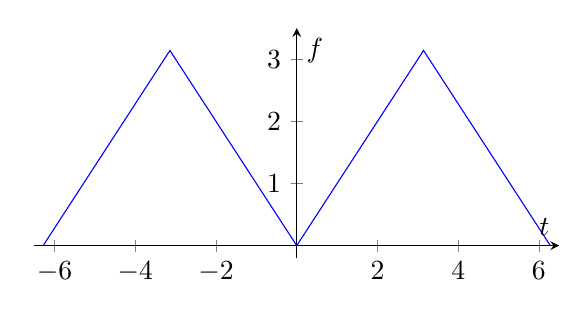
\begin{tikzpicture}\begin{axis}[width=.68\textwidth,height=4.5cm,axis lines=middle,xlabel={$t$},ylabel={$f$},samples=130,xmin=-6.5,xmax=6.5,ymin=-.2,ymax=3.5]
\addplot[blue]coordinates{(-6.283,0)(-3.142,3.142)(0,0)(3.142,3.142)(6.283,0)};\end{axis}\end{tikzpicture}\end{center}
\par\noindent{\small 依据：官方译审并补证（AI辅助）。}
\end{solution}

\begin{exercise}\label{cw:rec15-2}
用上一题 $f$ 驱动谐振子 $\ddot x+\omega_n^2x=f(t)$。何时存在周期解？若存在，写成 Fourier 级数。
\end{exercise}
\begin{solution}
当 $\omega_n\ge0$ 且 $\omega_n\notin\{0,1,3,5,\ldots\}$ 时，取
\[x_p=\frac\pi{2\omega_n^2}-\frac4\pi\sum_{k\text{奇}}\frac{\cos kt}{k^2(\omega_n^2-k^2)}.\]
固定非共振$\omega_n$时，尾项为$O(k^{-4})$，二阶导数项为$O(k^{-2})$，两者一致收敛，故可逐项二次求导并得到$f$，这确为$C^2$周期解。若$\omega_n$为奇整数，共振输入系数非零产生线性增长；若$\omega_n=0$，$x'(t+2\pi)-x'(t)=\int_t^{t+2\pi}f=\pi^2\ne0$，亦不可能周期。
\par\noindent{\small 依据：官方译审并补证（AI辅助）。}
\end{solution}

\begin{exercise}\label{cw:rec15-3}
改用圆频率$\omega>0$的$g(t)$驱动 $\ddot x+\omega_n^2x=g(t)$，求周期解及存在条件。
\end{exercise}
\begin{solution}
把每个频率改为$k\omega$，得到
\[x_p=\frac\pi{2\omega_n^2}-\frac4\pi\sum_{k\text{奇}}\frac{\cos(k\omega t)}{k^2[\omega_n^2-(k\omega)^2]}.
\]
存在条件是 $\omega_n>0$ 且不等于任何正奇数倍$\omega$。同上一题，尾项与二阶导数分别为$O(k^{-4})$、$O(k^{-2})$，可逐项核验；$\omega_n=0$ 时非零平均输入排除周期解。
\par\noindent{\small 依据：官方译审并补证（AI辅助）。}
\end{solution}

\begin{exercise}\label{cw:rec15-4}
固定$\omega$而调节自然圆频率$\omega_n$（例如调谐无线电电路）。在哪些值没有周期响应？当$\omega_n$略大或略小时响应如何变化？
\end{exercise}
\begin{solution}
非周期值为 $\omega_n=0$ 或 $k\omega$（$k$正奇数）。靠近非零共振时，频率$k\omega$的系数 $-4/[\pi k^2(\omega_n^2-k^2\omega^2)]$ 绝对值很大；略高于共振时此系数负，与该负余弦输入同相，略低时系数正，与该输入反相。靠近0时平均响应$\pi/(2\omega_n^2)$变得很大。精确共振的$t$增长项不能用大的有限稳态系数替代。
\par\noindent{\small 依据：官方译审并补证（AI辅助）。}
\end{solution}

\begin{exercise}\label{cw:rec15-5}
是否存在具有不止一个周期解的频率？给出条件。
\end{exercise}
\begin{solution}
一般解为 $x_p+C_1\cos\omega_nt+C_2\sin\omega_nt$。在非共振条件下，若 $\omega_n/\omega\in\mathbb Q$，齐次周期与输入周期可公度，任意$C_1,C_2$都给周期解，所以有无穷多个。例如$\omega_n=2\omega$。
若此比无理，则仅$C_1=C_2=0$给周期解：$x_p$含非零频率$\omega$项（连续周期函数的 Fourier 系数唯一），增加非零自然频率项后，一旦存在周期，两个非零频率都须是其基本频率的整数倍，矛盾。因此不能不加可公度条件便断言加任意齐次解仍周期。
\par\noindent{\small 依据：官方译审并补证（AI辅助）；修正任意齐次周期项可相加的缺失条件。}
\end{solution}

\originalchapter{习题课：阶跃、冲量、卷积与 Laplace 变换}
\originalsection{第16次习题课：广义导数与响应（4月6日）}
\begin{exercise}\label{cw:rec16-1}
令 $Q(t)=0$（$t<1$），$Q=2t-2$（$1<t<2$），$Q=2t-1$（$2<t<3$），$Q=5$（$t>3$）。
(a) 画图，判断是否分段光滑；(b) 求广义导数$q=Q'$并画图；(c) 举一个给出 $\dot x+kx=q$、静止初态的情境，可自选$k$甚至取负；(d) 举一个给出 $2\ddot x+4\dot x+4x=q$、静止初态的情境。
\end{exercise}
\begin{solution}
(a) 每段为一次函数或常数，端点有限，故分段光滑；$t=2$从2跳到3，跳幅1。
(b) $q=2u(t-1)-2u(t-3)+\delta(t-2)$；在$(1,3)$普通部分为2，外部为0，另有$t=2$的单位冲量。图的箭头高度仅标强度1，不把$\delta$当普通有限函数。
(c) 取$k=-r,r>0$，银行余额按年利率$r$连续增长；$t=1$到3以每年2单位存款，$t=2$另一次性存入1单位，之前无余额，即$\dot x-rx=q$。必须用$k=-r$才能表示正利息。
(d) 质量2、阻尼4、刚度4的静止弹簧系统受此外力：时间1到3恒力2，时间2施加总冲量1。冲量使速度跳$1/2$，位置连续。\begin{center}\begin{tikzpicture}\begin{axis}[width=.44\textwidth,height=3.8cm,axis lines=middle,xlabel={$t$},ylabel={$Q$},xmin=0,xmax=4,ymin=0,ymax=5.5]\addplot[blue]coordinates{(0,0)(1,0)(2,2)};\addplot[blue]coordinates{(2,3)(3,5)(4,5)};\draw[dashed](axis cs:2,2)--(axis cs:2,3);\end{axis}\end{tikzpicture}\begin{tikzpicture}\begin{axis}[width=.44\textwidth,height=3.8cm,axis lines=middle,xlabel={$t$},ylabel={$q$},xmin=0,xmax=4,ymin=0,ymax=5.5]\addplot[blue]coordinates{(0,0)(1,0)};\addplot[blue]coordinates{(1,2)(3,2)};\addplot[blue]coordinates{(3,0)(4,0)};\draw[red,->,thick](axis cs:2,2)--(axis cs:2,4)node[above]{强度1};\end{axis}\end{tikzpicture}\end{center}
\par\noindent{\small 依据：官方译审并补证（AI辅助）。}
\end{solution}

\begin{exercise}\label{cw:rec16-2}
求算子 $2D+I$ 的单位阶跃响应与单位冲量响应，并画图。
\end{exercise}
\begin{solution}
阶跃响应在$t>0$满足 $2\dot v+v=1,v(0+)=0$，解为 $v=u(t)(1-\ee^{-t/2})$。其广义导数 $w=\frac12u(t)\ee^{-t/2}$，原点无额外$\delta$，因为$v$连续。$w$的跳幅$1/2$使$(2D+I)w=\delta$。黑线为$v$、蓝线为$w$，$t<0$均为0。\begin{center}\begin{tikzpicture}\begin{axis}[width=.68\textwidth,height=4.5cm,axis lines=middle,xlabel={$t$},ylabel={响应},samples=130,xmin=0,xmax=7,ymin=0,ymax=1.1]
\addplot[black,domain=0:7]{1-exp(-x/2)};\addplot[blue,domain=0:7]{.5*exp(-x/2)};\end{axis}\end{tikzpicture}\end{center}
\par\noindent{\small 依据：官方译审并补证（AI辅助）。}
\end{solution}

\begin{exercise}\label{cw:rec16-3}
求 $D^2+2D$ 的单位冲量响应并画图。
\end{exercise}
\begin{solution}
冲量积分给 $w(0+)=0,w'(0+)=1$，$t>0$满足 $w''+2w'=0$。故 $w'=\ee^{-2t}$，$w=\frac12u(t)(1-\ee^{-2t})$。分布求导第二次在0产生系数1的$\delta$，普通部分抵消。\begin{center}\begin{tikzpicture}\begin{axis}[width=.68\textwidth,height=4.5cm,axis lines=middle,xlabel={$t$},ylabel={$w$},samples=130,xmin=0,xmax=4,ymin=0,ymax=.6]
\addplot[blue,domain=0:4]{(1-exp(-2*x))/2};\end{axis}\end{tikzpicture}\end{center}
\par\noindent{\small 依据：官方译审并补证（AI辅助）。}
\end{solution}

\begin{exercise}\label{cw:rec16-4}
利用上一题求 $\ddot x+2\dot x=3\delta(t-1)$ 的静止初态解。
\end{exercise}
\begin{solution}
时间不变性与线性性给 $x(t)=3w(t-1)=\frac32u(t-1)[1-\ee^{-2(t-1)}]$。时间1前为0，位置在1连续，速度从0跳到3；积分原方程穿过1可检验冲量强度恰为3。
\par\noindent{\small 依据：官方译审并补证（AI辅助）。}
\end{solution}

\originalsection{第17次习题课：卷积（4月8日）}
采用因果约定：所有函数在$t<0$为0，$f*g(t)=\int_0^tf(t-\tau)g(\tau)\dd\tau$。若$w$是$p(D)$的单位冲量响应，则静止初态响应为$w*q$。
\begin{exercise}\label{cw:rec17-1}
(a) 求 $t*u(t)$，并一般求$q*u$；(b) 求$u*t$，并一般求$u*q$。两者关系反映什么性质？
\end{exercise}
\begin{solution}
(a) $t*u=\int_0^t(t-\tau)\dd\tau=t^2/2$，$q*u=\int_0^tq(t-\tau)\dd\tau$。(b) $u*t=\int_0^t\tau\dd\tau=t^2/2$，$u*q=\int_0^tq(\tau)\dd\tau$。用$v=t-\tau$换元，两一般式相同；同样换元证明$f*g=g*f$，即卷积交换性。所有结果在$t<0$延为0。
\par\noindent{\small 依据：官方译审并补证（AI辅助）。}
\end{solution}

\begin{exercise}\label{cw:rec17-2}
哪一个微分算子$p(D)$的单位冲量响应是$u(t)$？上一题计算$u*q$是否验证了卷积响应结论？
\end{exercise}
\begin{solution}
$Du=\delta$，故$p(D)=D$。$x=u*q=\int_0^tq(\tau)\dd\tau$给原点前0，且$Dx=q$；普通连续$q$时由微积分基本定理成立，含冲量时由因果积分的广义导数成立。因此此算子确满足卷积响应结论。
\par\noindent{\small 依据：官方译审并补证（AI辅助）。}
\end{solution}

\begin{exercise}\label{cw:rec17-3}
(a) 若$f$在$a$连续，应如何理解$f(t)\delta(t-a)$？(b) 若$f$连续且$t<0$为0，解释$a\ge0$时$f*\delta(t-a)=f(t-a)$；说明$a=0$的含义。
\end{exercise}
\begin{solution}
(a) 作为测度乘连续函数，任意测试函数$\psi$满足 $\int\psi f\dd\delta_a=\psi(a)f(a)$，故乘积为$f(a)\delta(t-a)$。若坚持一般分布框架可先对光滑$f$定义，再用本题的点质量测度解释连续情形。(b) $t\ge a$ 时卷积抽样为$f(t-a)$，$t<a$时没有支持点，结果为0，与因果延拓$f(t-a)=0$一致。包括原点冲量时积分应从$0^-$开始，不能误取半个冲量。$a=0$给$f*\delta=f$，即卷积单位元。
\par\noindent{\small 依据：官方译审并补证（AI辅助）。}
\end{solution}

\begin{exercise}\label{cw:rec17-4}
(a) 核验 $u(t)\sin(\omega_nt)/\omega_n$ 是 $D^2+\omega_n^2I$ 的单位冲量响应；(b) 用共振 ERF 求 $\ddot x+x=\sin t,x(0)=\dot x(0)=0$；(c) 在 $t=2\pi n,n\in\mathbb N_{>0}$ 计算$\sin t*\sin t$，并与(b)核对，可用$\sin^2t=(1-\cos2t)/2$。
\end{exercise}
\begin{solution}
(a) 记普通部分$v=\sin\omega_nt/\omega_n$，$v(0)=0,v'(0)=1$，故$D^2(uv)=u v''+\delta$；加入$\omega_n^2uv$后普通项抵消，留下$\delta$。$\omega_n=0$时连续极限为$u(t)t$。
(b) 复替代$z''+z=\ee^{\ii t}$给$z_p=t\ee^{\ii t}/(2\ii)$，虚部$-t\cos t/2$；补齐初值后 $x=(\sin t-t\cos t)/2$。
(c) $\sin(2\pi n-\tau)=-\sin\tau$，所以卷积值为$-\int_0^{2\pi n}\sin^2\tau\dd\tau=-\pi n$。代入(b)也为$-\pi n$。两者不仅在这些点相同，卷积一般计算用积化和差得$(\sin t-t\cos t)/2$。
\par\noindent{\small 依据：官方译审并补证（AI辅助）。}
\end{solution}

\originalsection{第18次习题课：Laplace 变换（4月13日）}
本次变换按因果延拓从$0^-$积分，$\Lap[Df]=sF(s)$中的$D$为广义导数；对普通右导数则$\Lap[f_r']=sF-f(0+)$。所有公式在相应右半平面成立。
\begin{exercise}\label{cw:rec18-1}
从规则与表求 $u(t)\ee^{-t}(t^2+1)$ 的 Laplace 变换。
\end{exercise}
\begin{solution}
$\Lap[t^2+1]=2/s^3+1/s$；乘$\ee^{-t}$使$s$换成$s+1$，故 $F=2/(s+1)^3+1/(s+1)=(s^2+2s+3)/(s+1)^3$，$\Re s>-1$。
\par\noindent{\small 依据：官方译审并补证（AI辅助）。}
\end{solution}

\begin{exercise}\label{cw:rec18-2}
令 $f(t)=\ee^{-t}\cos3t$（隐含因果延拓）。求$F(s)$、广义导数$f'$及其变换，核验$t$导数规则。
\end{exercise}
\begin{solution}
$F=(s+1)/[(s+1)^2+9]$。原点跳幅为1，故 $Df=\delta-u(t)\ee^{-t}(\cos3t+3\sin3t)$。变换为 $1-(s+1)/[(s+1)^2+9]-9/[(s+1)^2+9]=s(s+1)/[(s+1)^2+9]=sF$，正好符合广义导数规则。
\par\noindent{\small 依据：官方译审并补证（AI辅助）。}
\end{solution}

\begin{exercise}\label{cw:rec18-3}
分别求 $(2s+1)/(s^2+9)$、$(s^2+2)/(s^3-s)$、$2/[s^2(s-1)]$ 的逆 Laplace 变换。
\end{exercise}
\begin{solution}
第一式分成$2s/(s^2+9)+(1/3)3/(s^2+9)$，故为$u(t)(2\cos3t+\sin3t/3)$。
第二式的部分分式为 $-2/s+(3/2)/(s-1)+(3/2)/(s+1)$，故为$u(t)[-2+\frac32(\ee^t+\ee^{-t})]$。
第三式为 $-2/s-2/s^2+2/(s-1)$，故为$2u(t)(\ee^t-1-t)$。每式分母通分即可核对系数，因果条件固定其右半平面解释。
\par\noindent{\small 依据：官方译审并补证（AI辅助）。}
\end{solution}

\begin{exercise}\label{cw:rec18-4}
用 Laplace 变换求$D+2I$的单位阶跃与单位冲量响应。
\end{exercise}
\begin{solution}
阶跃输入变换为$1/s$，$V=1/[s(s+2)]=\frac12(1/s-1/(s+2))$，故$v=\frac12u(t)(1-\ee^{-2t})$。冲量输入变换为1，$W=1/(s+2)$，故$w=u(t)\ee^{-2t}$。$v'=w$，且$w$原点跳幅1，均可检验。
\par\noindent{\small 依据：官方译审并补证（AI辅助）。}
\end{solution}

\begin{exercise}\label{cw:rec18-5}
用 Laplace 变换求 $\dot x+2x=t^2,x(0+)=1$。
\end{exercise}
\begin{solution}
对普通导数取变换：$(s+2)X-1=2/s^3$，故 $X=(s^3+2)/[s^3(s+2)]=1/s^3-1/(2s^2)+1/(4s)+3/[4(s+2)]$。逆变换给 $x=t^2/2-t/2+1/4+3\ee^{-2t}/4$，$t\ge0$。在0值为1，求导加$2x$后指数项抵消、多项式项为$t^2$。若使用因果广义导数，则方程右侧另加$\delta(t)$，结果相同。
\par\noindent{\small 依据：官方译审并补证（AI辅助）。}
\end{solution}

\originalsection{第19次习题课：Laplace 变换与初值（4月15日）}
\begin{exercise}\label{cw:rec19-1}
求$D+3I$的单位冲量响应。
\end{exercise}
\begin{solution}
$(s+3)W=1$，故$w=u(t)\ee^{-3t}$；跳幅1使广义导数产生单位冲量，普通部分满足$w'+3w=0$。
\par\noindent{\small 依据：官方译审并补证（AI辅助）。}
\end{solution}

\begin{exercise}\label{cw:rec19-2}
用 Laplace 变换求 $\dot x+3x=\ee^{-t}$ 的静止初值解$x(0)=0$。
\end{exercise}
\begin{solution}
$X=1/[(s+1)(s+3)]=\frac12[1/(s+1)-1/(s+3)]$，所以 $x=\frac12(\ee^{-t}-\ee^{-3t})$，$t\ge0$；在0值为0，代入方程得到输入$\ee^{-t}$。
\par\noindent{\small 依据：官方译审并补证（AI辅助）。}
\end{solution}

\begin{exercise}\label{cw:rec19-3}
用 Laplace 变换求 $D^3+D$ 的单位冲量响应。
\end{exercise}
\begin{solution}
$W=1/[s(s^2+1)]=1/s-s/(s^2+1)$，故$w=u(t)(1-\cos t)$。普通部分满足$w^{(3)}+w'=0$；$w(0)=w'(0)=0,w''(0)=1$，所以三阶广义导数在0恰产生$\delta$。
\par\noindent{\small 依据：官方译审并补证（AI辅助）。}
\end{solution}

\begin{exercise}\label{cw:rec19-4}
(a) 用普通导数规则求 $x_r'+3x=1,x(0+)=2$；(b) 以 $x(0-)=0$，把原点跳跃写为 $Dx+3x=u(t)+2\delta(t)$，再求解。
\end{exercise}
\begin{solution}
(a) $(s+3)X-2=1/s$，$X=1/[s(s+3)]+2/(s+3)$，故$x=1/3+5\ee^{-3t}/3$，$t\ge0$。(b) 广义规则给$(s+3)X=1/s+2$，同一变换；因果解为$u(t)(1/3+5\ee^{-3t}/3)$。原点跳幅2验证了输入冲量系数，原点后普通方程一致。
\par\noindent{\small 依据：官方译审并补证（AI辅助）。}
\end{solution}

\originalchapter{习题课：线性系统与非线性相图}
\originalsection{第21次习题课：矩阵与一阶线性系统（4月27日）}
\begin{exercise}\label{cw:rec21-1}
计算四个矩阵乘积：
\[[1\quad2]\binom xy,\qquad\binom12[x\quad y],\qquad\begin{pmatrix}a&b\\c&d\end{pmatrix}\binom xy,\qquad\begin{pmatrix}1&2\\3&4\end{pmatrix}\begin{pmatrix}x&u\\y&v\end{pmatrix}.\]
\end{exercise}
\begin{solution}
按照行乘列，结果依次为标量$x+2y$、外积矩阵$\begin{pmatrix}x&y\\2x&2y\end{pmatrix}$、列向量$\binom{ax+by}{cx+dy}$、矩阵$\begin{pmatrix}x+2y&u+2v\\3x+4y&3u+4v\end{pmatrix}$。第二个乘积次序与第一个不同，输出尺寸亦不同。
\par\noindent{\small 依据：官方译审并补证（AI辅助）。}
\end{solution}

\begin{exercise}\label{cw:rec21-2}
矩阵$A$把单位方形顶点 $0,e_1,e_1+e_2,e_2$ 送至$0,Ae_1,A(e_1+e_2),Ae_2$。对以下五个$A$依序连接这些像点，画图并描述变换：
\[\begin{pmatrix}1&0\\0&2\end{pmatrix},\quad\begin{pmatrix}1&1\\0&1\end{pmatrix},\quad\begin{pmatrix}1&0\\0&-1\end{pmatrix},\quad\begin{pmatrix}0&1\\1&0\end{pmatrix},\quad\begin{pmatrix}1&1\\1&-1\end{pmatrix}.\]
\end{exercise}
\begin{solution}
像点依次为 $(0,0),(1,0),(1,2),(0,2)$；$(0,0),(1,0),(2,1),(1,1)$；\par $(0,0),(1,0),(1,-1),(0,-1)$；$(0,0),(0,1),(1,1),(1,0)$；\par $(0,0),(1,1),(2,0),(1,-1)$。各组均再闭合回原点。
对应为竖直放大2倍、水平剪切、关于$x$轴反射、关于$y=x$反射、以及先关于$x$轴反射再逆时针旋转$\pi/4$并放大$\sqrt2$。最后一个次序可由 $A=\sqrt2 R_{\pi/4}\diag(1,-1)$核验。\begin{center}\begin{tikzpicture}\begin{axis}[width=.28\textwidth,height=3.5cm,axis lines=middle,title={竖直伸长},xmin=-1.5,xmax=2.5,ymin=-1.5,ymax=2.5,xlabel={$x$},ylabel={$y$}]\addplot[blue,mark=*]coordinates {(0,0) (1,0) (1,2) (0,2) (0,0)};\end{axis}\end{tikzpicture}\begin{tikzpicture}\begin{axis}[width=.28\textwidth,height=3.5cm,axis lines=middle,title={剪切},xmin=-1.5,xmax=2.5,ymin=-1.5,ymax=2.5,xlabel={$x$},ylabel={$y$}]\addplot[blue,mark=*]coordinates {(0,0) (1,0) (2,1) (1,1) (0,0)};\end{axis}\end{tikzpicture}\begin{tikzpicture}\begin{axis}[width=.28\textwidth,height=3.5cm,axis lines=middle,title={关于横轴反射},xmin=-1.5,xmax=2.5,ymin=-1.5,ymax=2.5,xlabel={$x$},ylabel={$y$}]\addplot[blue,mark=*]coordinates {(0,0) (1,0) (1,-1) (0,-1) (0,0)};\end{axis}\end{tikzpicture}\par\begin{tikzpicture}\begin{axis}[width=.28\textwidth,height=3.5cm,axis lines=middle,title={交换坐标},xmin=-1.5,xmax=2.5,ymin=-1.5,ymax=2.5,xlabel={$x$},ylabel={$y$}]\addplot[blue,mark=*]coordinates {(0,0) (0,1) (1,1) (1,0) (0,0)};\end{axis}\end{tikzpicture}\begin{tikzpicture}\begin{axis}[width=.28\textwidth,height=3.5cm,axis lines=middle,title={反射、旋转与伸长},xmin=-1.5,xmax=2.5,ymin=-1.5,ymax=2.5,xlabel={$x$},ylabel={$y$}]\addplot[blue,mark=*]coordinates {(0,0) (1,1) (2,0) (1,-1) (0,0)};\end{axis}\end{tikzpicture}\end{center}
\par\noindent{\small 依据：官方译审并补证（AI辅助）。}
\end{solution}

\begin{exercise}\label{cw:rec21-3}
求$\ddot x+2\dot x+2x=0$的伴随矩阵$A$，写两个实独立解。令$x_1(0)=0,\dot x_1(0)=1$，求$x_1$及$u_1=(x_1,\dot x_1)^T$、$u_1(0)$；画$x_1,\dot x_1$时间图与$u_1$轨迹，比较。再画几条轨迹，特别是$u_2(0)=e_1$的轨迹。轨迹穿越$x$轴时角度为何？
\end{exercise}
\begin{solution}
设$v=\dot x$，$\dot u=Au$，$A=\begin{pmatrix}0&1\\-2&-2\end{pmatrix}$。特征根$-1\pm\ii$给$\ee^{-t}\cos t,\ee^{-t}\sin t$。
$x_1=\ee^{-t}\sin t$，$u_1=\ee^{-t}(\sin t,\cos t-\sin t)^T$，初值$e_2$。另一规范解$x_2=\ee^{-t}(\cos t+\sin t)$，$u_2=\ee^{-t}(\cos t+\sin t,-2\sin t)^T$，初值$e_1$。它们的线性组合给整个相图。
时间图中黑线为$x_1$、蓝线为$\dot x_1$；相图把同一时刻的二者作为坐标，向原点顺时针螺旋。在$x$轴上$v=0$，速度$(\dot x,\dot v)=(0,-2x)$竖直，故除平衡点外都垂直穿越，夹角$\pi/2$。\begin{center}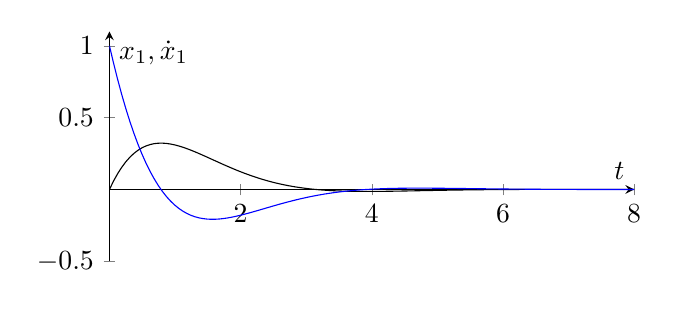
\begin{tikzpicture}\begin{axis}[width=.68\textwidth,height=4.5cm,axis lines=middle,xlabel={$t$},ylabel={$x_1,\dot x_1$},samples=130,xmin=0,xmax=8,ymin=-.5,ymax=1.1]
\addplot[black,domain=0:8]{exp(-x)*sin(deg(x))};\addplot[blue,domain=0:8]{exp(-x)*(cos(deg(x))-sin(deg(x)))};\end{axis}\end{tikzpicture}\end{center}\begin{center}\begin{tikzpicture}\begin{axis}[width=.5\textwidth,height=3.8cm,axis lines=middle,title={伴随系统相图},xlabel={$x$},ylabel={$y$},xmin=-2.4,xmax=2.4,ymin=-2.4,ymax=2.4,clip=true]\addplot[blue,no marks] coordinates {(0.02346,3.05467) (0.32628,2.40884) (0.56155,1.83847) (0.73754,1.34114) (0.86216,0.91327) (0.94290,0.55049) (0.98671,0.24783) (1.00000,0.00000) (0.98854,-0.19844) (0.95753,-0.35296) (0.91154,-0.46889) (0.85457,-0.55136) (0.79007,-0.60521) (0.72097,-0.63496) (0.64971,-0.64476) (0.57829,-0.63835) (0.50833,-0.61912) (0.44107,-0.59004) (0.37747,-0.55372) (0.31821,-0.51240) (0.26372,-0.46799) (0.21426,-0.42210) (0.16993,-0.37602) (0.13067,-0.33081) (0.09635,-0.28731) (0.06674,-0.24612) (0.04156,-0.20770) (0.02047,-0.17235) (0.00313,-0.14024) (-0.01082,-0.11142) (-0.02175,-0.08589) (-0.03002,-0.06355) (-0.03598,-0.04425) (-0.03996,-0.02782) (-0.04226,-0.01405) (-0.04317,-0.00272) (-0.04295,0.00642) (-0.04182,0.01360) (-0.03999,0.01904) (-0.03764,0.02298) (-0.03493,0.02563) (-0.03199,0.02718) (-0.02893,0.02782) (-0.02583,0.02772) (-0.02279,0.02703) (-0.01984,0.02588) (-0.01705,0.02438) (-0.01443,0.02265) (-0.01202,0.02076) (-0.00982,0.01879) (-0.00785,0.01679) (-0.00609,0.01483) (-0.00455,0.01292)};\draw[blue,->] (axis cs:0.94727,-0.38536)--(axis cs:0.89377,-0.49956);\addplot[blue,no marks] coordinates {(-0.02346,-3.05467) (-0.32628,-2.40884) (-0.56155,-1.83847) (-0.73754,-1.34114) (-0.86216,-0.91327) (-0.94290,-0.55049) (-0.98671,-0.24783) (-1.00000,0.00000) (-0.98854,0.19844) (-0.95753,0.35296) (-0.91154,0.46889) (-0.85457,0.55136) (-0.79007,0.60521) (-0.72097,0.63496) (-0.64971,0.64476) (-0.57829,0.63835) (-0.50833,0.61912) (-0.44107,0.59004) (-0.37747,0.55372) (-0.31821,0.51240) (-0.26372,0.46799) (-0.21426,0.42210) (-0.16993,0.37602) (-0.13067,0.33081) (-0.09635,0.28731) (-0.06674,0.24612) (-0.04156,0.20770) (-0.02047,0.17235) (-0.00313,0.14024) (0.01082,0.11142) (0.02175,0.08589) (0.03002,0.06355) (0.03598,0.04425) (0.03996,0.02782) (0.04226,0.01405) (0.04317,0.00272) (0.04295,-0.00642) (0.04182,-0.01360) (0.03999,-0.01904) (0.03764,-0.02298) (0.03493,-0.02563) (0.03199,-0.02718) (0.02893,-0.02782) (0.02583,-0.02772) (0.02279,-0.02703) (0.01984,-0.02588) (0.01705,-0.02438) (0.01443,-0.02265) (0.01202,-0.02076) (0.00982,-0.01879) (0.00785,-0.01679) (0.00609,-0.01483) (0.00455,-0.01292)};\draw[blue,->] (axis cs:-0.94727,0.38536)--(axis cs:-0.89377,0.49956);\addplot[blue,no marks] coordinates {(-1.88847,3.42156) (-1.52734,3.07813) (-1.20442,2.73512) (-0.91924,2.40003) (-0.67057,2.07868) (-0.45664,1.77543) (-0.27524,1.49338) (-0.12391,1.23454) (0.00000,1.00000) (0.09922,0.79010) (0.17648,0.60457) (0.23445,0.44265) (0.27568,0.30321) (0.30261,0.18486) (0.31748,0.08601) (0.32238,0.00495) (0.31918,-0.06006) (0.30956,-0.11079) (0.29502,-0.14897) (0.27686,-0.17624) (0.25620,-0.19419) (0.23400,-0.20427) (0.21105,-0.20783) (0.18801,-0.20609) (0.16541,-0.20014) (0.14365,-0.19095) (0.12306,-0.17938) (0.10385,-0.16615) (0.08618,-0.15188) (0.07012,-0.13710) (0.05571,-0.12224) (0.04294,-0.10764) (0.03177,-0.09357) (0.02213,-0.08023) (0.01391,-0.06778) (0.00703,-0.05631) (0.00136,-0.04589) (-0.00321,-0.03653) (-0.00680,-0.02822) (-0.00952,-0.02095) (-0.01149,-0.01466) (-0.01281,-0.00930) (-0.01359,-0.00481) (-0.01391,-0.00110) (-0.01386,0.00189) (-0.01352,0.00424) (-0.01294,0.00603) (-0.01219,0.00734) (-0.01132,0.00822) (-0.01038,0.00874) (-0.00939,0.00896) (-0.00840,0.00895) (-0.00741,0.00873) (-0.00646,0.00837)};\draw[blue,->] (axis cs:0.19268,0.56191)--(axis cs:0.24978,0.39421);\addplot[blue,no marks] coordinates {(1.88847,-3.42156) (1.52734,-3.07813) (1.20442,-2.73512) (0.91924,-2.40003) (0.67057,-2.07868) (0.45664,-1.77543) (0.27524,-1.49338) (0.12391,-1.23454) (0.00000,-1.00000) (-0.09922,-0.79010) (-0.17648,-0.60457) (-0.23445,-0.44265) (-0.27568,-0.30321) (-0.30261,-0.18486) (-0.31748,-0.08601) (-0.32238,-0.00495) (-0.31918,0.06006) (-0.30956,0.11079) (-0.29502,0.14897) (-0.27686,0.17624) (-0.25620,0.19419) (-0.23400,0.20427) (-0.21105,0.20783) (-0.18801,0.20609) (-0.16541,0.20014) (-0.14365,0.19095) (-0.12306,0.17938) (-0.10385,0.16615) (-0.08618,0.15188) (-0.07012,0.13710) (-0.05571,0.12224) (-0.04294,0.10764) (-0.03177,0.09357) (-0.02213,0.08023) (-0.01391,0.06778) (-0.00703,0.05631) (-0.00136,0.04589) (0.00321,0.03653) (0.00680,0.02822) (0.00952,0.02095) (0.01149,0.01466) (0.01281,0.00930) (0.01359,0.00481) (0.01391,0.00110) (0.01386,-0.00189) (0.01352,-0.00424) (0.01294,-0.00603) (0.01219,-0.00734) (0.01132,-0.00822) (0.01038,-0.00874) (0.00939,-0.00896) (0.00840,-0.00895) (0.00741,-0.00873) (0.00646,-0.00837)};\draw[blue,->] (axis cs:-0.19268,-0.56191)--(axis cs:-0.24978,-0.39421);\addplot[blue,no marks] coordinates {(0.06697,3.41982) (0.40552,2.68870) (0.66765,2.04387) (0.86280,1.48237) (1.00000,1.00000) (1.08777,0.59165) (1.13401,0.25161) (1.14598,-0.02624) (1.13025,-0.24815) (1.09268,-0.42035) (1.03845,-0.54896) (0.97209,-0.63981) (0.89747,-0.69841) (0.81789,-0.72991) (0.73609,-0.73901) (0.65433,-0.72996) (0.57441,-0.70659) (0.49772,-0.67227) (0.42531,-0.62993) (0.35794,-0.58210) (0.29608,-0.53095) (0.24000,-0.47826) (0.18980,-0.42550) (0.14541,-0.37385) (0.10665,-0.32424) (0.07325,-0.27734) (0.04490,-0.23366) (0.02120,-0.19353) (0.00175,-0.15711) (-0.01386,-0.12448) (-0.02605,-0.09560) (-0.03524,-0.07037) (-0.04182,-0.04860) (-0.04616,-0.03010) (-0.04862,-0.01463) (-0.04951,-0.00191) (-0.04913,0.00832) (-0.04774,0.01632) (-0.04558,0.02237) (-0.04284,0.02672) (-0.03969,0.02961) (-0.03630,0.03127) (-0.03278,0.03191) (-0.02924,0.03172) (-0.02576,0.03086) (-0.02240,0.02950) (-0.01922,0.02775) (-0.01624,0.02574) (-0.01350,0.02356) (-0.01101,0.02129)};\draw[blue,->] (axis cs:1.13995,0.17655)--(axis cs:1.14355,-0.10535);\addplot[blue,no marks] coordinates {(-0.06697,-3.41982) (-0.40552,-2.68870) (-0.66765,-2.04387) (-0.86280,-1.48237) (-1.00000,-1.00000) (-1.08777,-0.59165) (-1.13401,-0.25161) (-1.14598,0.02624) (-1.13025,0.24815) (-1.09268,0.42035) (-1.03845,0.54896) (-0.97209,0.63981) (-0.89747,0.69841) (-0.81789,0.72991) (-0.73609,0.73901) (-0.65433,0.72996) (-0.57441,0.70659) (-0.49772,0.67227) (-0.42531,0.62993) (-0.35794,0.58210) (-0.29608,0.53095) (-0.24000,0.47826) (-0.18980,0.42550) (-0.14541,0.37385) (-0.10665,0.32424) (-0.07325,0.27734) (-0.04490,0.23366) (-0.02120,0.19353) (-0.00175,0.15711) (0.01386,0.12448) (0.02605,0.09560) (0.03524,0.07037) (0.04182,0.04860) (0.04616,0.03010) (0.04862,0.01463) (0.04951,0.00191) (0.04913,-0.00832) (0.04774,-0.01632) (0.04558,-0.02237) (0.04284,-0.02672) (0.03969,-0.02961) (0.03630,-0.03127) (0.03278,-0.03191) (0.02924,-0.03172) (0.02576,-0.03086) (0.02240,-0.02950) (0.01922,-0.02775) (0.01624,-0.02574) (0.01350,-0.02356) (0.01101,-0.02129)};\draw[blue,->] (axis cs:-1.13995,-0.17655)--(axis cs:-1.14355,0.10535);\end{axis}\end{tikzpicture}\end{center}
\par\noindent{\small 依据：官方译审并补证（AI辅助）。}
\end{solution}

\begin{exercise}\label{cw:rec21-4}
若$(a+b\ii)(x+y\ii)=v+w\ii$，求把$(x,y)^T$送到$(v,w)^T$的实矩阵；再取$a+b\ii=2,\ii,1+\ii$，分别写矩阵并画单位方形的像。
\end{exercise}
\begin{solution}
展开得$v=ax-by,w=bx+ay$，所以$A=\begin{pmatrix}a&-b\\b&a\end{pmatrix}$。三例分别为$2I,\begin{pmatrix}0&-1\\1&0\end{pmatrix},\begin{pmatrix}1&-1\\1&1\end{pmatrix}$，即放大2倍、逆时针旋转$\pi/2$、逆时针旋转$\pi/4$并放大$\sqrt2$。\begin{center}\begin{tikzpicture}\begin{axis}[width=.28\textwidth,height=3.5cm,axis lines=middle,title={乘以2},xmin=-1.5,xmax=2.5,ymin=-1.5,ymax=2.5,xlabel={$x$},ylabel={$y$}]\addplot[blue,mark=*]coordinates {(0,0) (2,0) (2,2) (0,2) (0,0)};\end{axis}\end{tikzpicture}\begin{tikzpicture}\begin{axis}[width=.28\textwidth,height=3.5cm,axis lines=middle,title={乘以$\ii$},xmin=-1.5,xmax=2.5,ymin=-1.5,ymax=2.5,xlabel={$x$},ylabel={$y$}]\addplot[blue,mark=*]coordinates {(0,0) (0,1) (-1,1) (-1,0) (0,0)};\end{axis}\end{tikzpicture}\begin{tikzpicture}\begin{axis}[width=.28\textwidth,height=3.5cm,axis lines=middle,title={乘以$1+\ii$},xmin=-1.5,xmax=2.5,ymin=-1.5,ymax=2.5,xlabel={$x$},ylabel={$y$}]\addplot[blue,mark=*]coordinates {(0,0) (1,1) (0,2) (-1,1) (0,0)};\end{axis}\end{tikzpicture}\end{center}
\par\noindent{\small 依据：官方译审并补证（AI辅助）。}
\end{solution}

\originalsection{第22次习题课：特征值与特征向量（4月29日）}
\begin{exercise}\label{cw:rec22-1}
解系统$\dot x=-5x-3y,\dot y=6x+4y$。
(a) 写系数矩阵、迹、行列式、$p_A(\lambda)=\det(A-\lambda I)$及其系数关系；(b) 求特征值和非零特征向量；(c) 画特征线及时间方向，解释每线为何分成三条轨迹；取线上非零点，写所有经过它的解；(d) 把初值$u(0)=(1,0)^T$分解，写解、画轨迹，再写具有同一轨迹的所有解；(e) 补完整相图。
\end{exercise}
\begin{solution}
(a) $A=\begin{pmatrix}-5&-3\\6&4\end{pmatrix}$，$\tau=-1,\Delta=-2$，$p_A=\lambda^2-\tau\lambda+\Delta=\lambda^2+\lambda-2$。
(b) $\lambda_+=1,v_+=(1,-2)^T$；$\lambda_-=-2,v_-=(1,-1)^T$，直接乘矩阵核验。
(c) 特征线$y=-2x$向外，$y=-x$向内；线上解为$ce^{\lambda t}v$。因指数始终正，正半线、原点、负半线是三条不同轨迹。若固定非零点$p=cv$，所有在某时刻$t_0$经过$p$的解为$u(t)=\ee^{\lambda(t-t_0)}p$，$t_0\in\mathbb R$。
(d) $(1,0)^T=-v_++2v_-$，故 $u_0(t)=(-\ee^t+2\ee^{-2t},2\ee^t-2\ee^{-2t})^T$；同一轨迹的所有参数化解为$u_0(t-t_0)$，相当于$c_+=-\ee^{-t_0},c_-=2\ee^{2t_0}$。
(e) 一般解$u=c_+\ee^tv_++c_-\ee^{-2t}v_-$，相图为鞍点；非特征轨迹前向沿不稳定线远离，反向沿稳定线远离。图的箭头为时间正向。\begin{center}\begin{tikzpicture}\begin{axis}[width=.55\textwidth,height=3.8cm,axis lines=middle,title={稳定线$y=-x$},xlabel={$x$},ylabel={$y$},xmin=-2.4,xmax=2.4,ymin=-2.4,ymax=2.4,clip=true]\addplot[blue,no marks] coordinates {(3.17894,-2.46241) (2.72835,-1.97089) (2.31851,-1.51777) (1.94474,-1.09826) (1.60286,-0.70802) (1.28908,-0.34312) (1.00000,0.00000) (0.73255,0.32458) (0.48396,0.63356) (0.25170,0.92966) (0.03351,1.21534) (-0.17269,1.49288) (-0.36878,1.76439) (-0.55649,2.03183) (-0.73740,2.29702) (-0.91296,2.56168) (-1.08452,2.82743) (-1.25333,3.09581) (-1.42054,3.36827)};\draw[blue,->] (axis cs:-0.07096,1.35499)--(axis cs:-0.49351,1.94124);\addplot[blue,no marks] coordinates {(3.39472,-3.39472) (3.03773,-3.03773) (2.71828,-2.71828) (2.43243,-2.43243) (2.17663,-2.17663) (1.94773,-1.94773) (1.74291,-1.74291) (1.55962,-1.55962) (1.39561,-1.39561) (1.24885,-1.24885) (1.11752,-1.11752) (1.00000,-1.00000) (0.89484,-0.89484) (0.80074,-0.80074) (0.71653,-0.71653) (0.64118,-0.64118) (0.57375,-0.57375) (0.51342,-0.51342) (0.45943,-0.45943) (0.41111,-0.41111) (0.36788,-0.36788) (0.32919,-0.32919) (0.29457,-0.29457) (0.26360,-0.26360) (0.23588,-0.23588) (0.21107,-0.21107) (0.18888,-0.18888) (0.16901,-0.16901) (0.15124,-0.15124) (0.13534,-0.13534) (0.12110,-0.12110) (0.10837,-0.10837) (0.09697,-0.09697) (0.08677,-0.08677) (0.07765,-0.07765) (0.06948,-0.06948) (0.06218,-0.06218) (0.05564,-0.05564) (0.04979,-0.04979) (0.04455,-0.04455) (0.03987,-0.03987) (0.03567,-0.03567) (0.03192,-0.03192) (0.02857,-0.02857) (0.02556,-0.02556) (0.02287,-0.02287) (0.02047,-0.02047) (0.01832,-0.01832)};\draw[blue,->] (axis cs:0.60653,-0.60653)--(axis cs:0.47711,-0.47711);\addplot[blue,no marks] coordinates {(-3.39472,3.39472) (-3.03773,3.03773) (-2.71828,2.71828) (-2.43243,2.43243) (-2.17663,2.17663) (-1.94773,1.94773) (-1.74291,1.74291) (-1.55962,1.55962) (-1.39561,1.39561) (-1.24885,1.24885) (-1.11752,1.11752) (-1.00000,1.00000) (-0.89484,0.89484) (-0.80074,0.80074) (-0.71653,0.71653) (-0.64118,0.64118) (-0.57375,0.57375) (-0.51342,0.51342) (-0.45943,0.45943) (-0.41111,0.41111) (-0.36788,0.36788) (-0.32919,0.32919) (-0.29457,0.29457) (-0.26360,0.26360) (-0.23588,0.23588) (-0.21107,0.21107) (-0.18888,0.18888) (-0.16901,0.16901) (-0.15124,0.15124) (-0.13534,0.13534) (-0.12110,0.12110) (-0.10837,0.10837) (-0.09697,0.09697) (-0.08677,0.08677) (-0.07765,0.07765) (-0.06948,0.06948) (-0.06218,0.06218) (-0.05564,0.05564) (-0.04979,0.04979) (-0.04455,0.04455) (-0.03987,0.03987) (-0.03567,0.03567) (-0.03192,0.03192) (-0.02857,0.02857) (-0.02556,0.02556) (-0.02287,0.02287) (-0.02047,0.02047) (-0.01832,0.01832)};\draw[blue,->] (axis cs:-0.60653,0.60653)--(axis cs:-0.47711,0.47711);\addplot[blue,no marks] coordinates {(0.36788,-0.73576) (0.38890,-0.77779) (0.41111,-0.82222) (0.43460,-0.86920) (0.45943,-0.91885) (0.48567,-0.97134) (0.51342,-1.02683) (0.54275,-1.08549) (0.57375,-1.14751) (0.60653,-1.21306) (0.64118,-1.28236) (0.67781,-1.35562) (0.71653,-1.43306) (0.75747,-1.51493) (0.80074,-1.60147) (0.84648,-1.69296) (0.89484,-1.78968) (0.94596,-1.89192) (1.00000,-2.00000) (1.05713,-2.11426) (1.11752,-2.23504) (1.18136,-2.36272) (1.24885,-2.49770) (1.32019,-2.64039) (1.39561,-2.79122) (1.47534,-2.95068) (1.55962,-3.11925) (1.64872,-3.29744) (1.74291,-3.48582)};\addplot[blue,no marks] coordinates {(-0.36788,0.73576) (-0.38890,0.77779) (-0.41111,0.82222) (-0.43460,0.86920) (-0.45943,0.91885) (-0.48567,0.97134) (-0.51342,1.02683) (-0.54275,1.08549) (-0.57375,1.14751) (-0.60653,1.21306) (-0.64118,1.28236) (-0.67781,1.35562) (-0.71653,1.43306) (-0.75747,1.51493) (-0.80074,1.60147) (-0.84648,1.69296) (-0.89484,1.78968) (-0.94596,1.89192) (-1.00000,2.00000) (-1.05713,2.11426) (-1.11752,2.23504) (-1.18136,2.36272) (-1.24885,2.49770) (-1.32019,2.64039) (-1.39561,2.79122) (-1.47534,2.95068) (-1.55962,3.11925) (-1.64872,3.29744) (-1.74291,3.48582)};\addplot[blue,no marks] coordinates {(3.28025,-2.76683) (2.85198,-2.30923) (2.46398,-1.89022) (2.11175,-1.50522) (1.79125,-1.15006) (1.49882,-0.82101) (1.23120,-0.51467) (0.98544,-0.22798) (0.75889,0.04185) (0.54913,0.29735) (0.35401,0.54083) (0.17156,0.77440) (0.00000,1.00000) (-0.16229,1.21942) (-0.31678,1.43430) (-0.46483,1.64619) (-0.60767,1.85652) (-0.74644,2.06663) (-0.88220,2.27781) (-1.01591,2.49126) (-1.14851,2.70813) (-1.28084,2.92956) (-1.41372,3.15663) (-1.54790,3.39038)};\addplot[blue,no marks] coordinates {(-3.28025,2.76683) (-2.85198,2.30923) (-2.46398,1.89022) (-2.11175,1.50522) (-1.79125,1.15006) (-1.49882,0.82101) (-1.23120,0.51467) (-0.98544,0.22798) (-0.75889,-0.04185) (-0.54913,-0.29735) (-0.35401,-0.54083) (-0.17156,-0.77440) (0.00000,-1.00000) (0.16229,-1.21942) (0.31678,-1.43430) (0.46483,-1.64619) (0.60767,-1.85652) (0.74644,-2.06663) (0.88220,-2.27781) (1.01591,-2.49126) (1.14851,-2.70813) (1.28084,-2.92956) (1.41372,-3.15663) (1.54790,-3.39038)};\end{axis}\end{tikzpicture}\end{center}
\par\noindent{\small 依据：官方译审并补证（AI辅助）。}
\end{solution}

\begin{exercise}\label{cw:rec22-2}
对$\dot x=4x+3y,\dot y=-6x-5y$，完成第1题同一(a)--(e)序列，包括初值$(1,0)^T$及所有同轨迹解。
\end{exercise}
\begin{solution}
(a) $B=\begin{pmatrix}4&3\\-6&-5\end{pmatrix}$，迹$-1$、行列式$-2$，仍有$p_B=\lambda^2+\lambda-2$。
(b) $\lambda_+=1,w_+=(1,-1)^T$；$\lambda_-=-2,w_-=(1,-2)^T$。
(c) 此时$y=-x$向外，$y=-2x$向内；每线仍为正半线、零点、负半线三轨迹。经过$p=cw_\pm\ne0$的所有解为$\ee^{\lambda_\pm(t-t_0)}p$。
(d) $(1,0)^T=2w_+-w_-$，故 $v_0(t)=(2\ee^t-\ee^{-2t},-2\ee^t+2\ee^{-2t})^T$；所有同轨迹解为$v_0(t-t_0)$。
(e) 通解$c_+\ee^tw_++c_-\ee^{-2t}w_-$，仍是鞍点，但两条特征线的稳定性交换；不能把整个向量场简单说成$-A$，因为两矩阵的迹相同。\begin{center}\begin{tikzpicture}\begin{axis}[width=.55\textwidth,height=3.8cm,axis lines=middle,title={稳定线$y=-2x$},xlabel={$x$},ylabel={$y$},xmin=-2.4,xmax=2.4,ymin=-2.4,ymax=2.4,clip=true]\addplot[blue,no marks] coordinates {(-0.82101,2.99764) (-0.51467,2.46241) (-0.22798,1.97089) (0.04185,1.51777) (0.29735,1.09826) (0.54083,0.70802) (0.77440,0.34312) (1.00000,0.00000) (1.21942,-0.32458) (1.43430,-0.63356) (1.64619,-0.92966) (1.85652,-1.21534) (2.06663,-1.49288) (2.27781,-1.76439) (2.49126,-2.03183) (2.70813,-2.29702) (2.92956,-2.56168) (3.15663,-2.82743) (3.39038,-3.09581)};\addplot[blue,no marks] coordinates {(0.36788,-0.36788) (0.38890,-0.38890) (0.41111,-0.41111) (0.43460,-0.43460) (0.45943,-0.45943) (0.48567,-0.48567) (0.51342,-0.51342) (0.54275,-0.54275) (0.57375,-0.57375) (0.60653,-0.60653) (0.64118,-0.64118) (0.67781,-0.67781) (0.71653,-0.71653) (0.75747,-0.75747) (0.80074,-0.80074) (0.84648,-0.84648) (0.89484,-0.89484) (0.94596,-0.94596) (1.00000,-1.00000) (1.05713,-1.05713) (1.11752,-1.11752) (1.18136,-1.18136) (1.24885,-1.24885) (1.32019,-1.32019) (1.39561,-1.39561) (1.47534,-1.47534) (1.55962,-1.55962) (1.64872,-1.64872) (1.74291,-1.74291) (1.84248,-1.84248) (1.94773,-1.94773) (2.05900,-2.05900) (2.17663,-2.17663) (2.30098,-2.30098) (2.43243,-2.43243) (2.57138,-2.57138) (2.71828,-2.71828) (2.87357,-2.87357) (3.03773,-3.03773) (3.21127,-3.21127) (3.39472,-3.39472)};\draw[blue,->] (axis cs:1.28403,-1.28403)--(axis cs:1.44773,-1.44773);\addplot[blue,no marks] coordinates {(-0.36788,0.36788) (-0.38890,0.38890) (-0.41111,0.41111) (-0.43460,0.43460) (-0.45943,0.45943) (-0.48567,0.48567) (-0.51342,0.51342) (-0.54275,0.54275) (-0.57375,0.57375) (-0.60653,0.60653) (-0.64118,0.64118) (-0.67781,0.67781) (-0.71653,0.71653) (-0.75747,0.75747) (-0.80074,0.80074) (-0.84648,0.84648) (-0.89484,0.89484) (-0.94596,0.94596) (-1.00000,1.00000) (-1.05713,1.05713) (-1.11752,1.11752) (-1.18136,1.18136) (-1.24885,1.24885) (-1.32019,1.32019) (-1.39561,1.39561) (-1.47534,1.47534) (-1.55962,1.55962) (-1.64872,1.64872) (-1.74291,1.74291) (-1.84248,1.84248) (-1.94773,1.94773) (-2.05900,2.05900) (-2.17663,2.17663) (-2.30098,2.30098) (-2.43243,2.43243) (-2.57138,2.57138) (-2.71828,2.71828) (-2.87357,2.87357) (-3.03773,3.03773) (-3.21127,3.21127) (-3.39472,3.39472)};\draw[blue,->] (axis cs:-1.28403,1.28403)--(axis cs:-1.44773,1.44773);\addplot[blue,no marks] coordinates {(1.74291,-3.48582) (1.55962,-3.11925) (1.39561,-2.79122) (1.24885,-2.49770) (1.11752,-2.23504) (1.00000,-2.00000) (0.89484,-1.78968) (0.80074,-1.60147) (0.71653,-1.43306) (0.64118,-1.28236) (0.57375,-1.14751) (0.51342,-1.02683) (0.45943,-0.91885) (0.41111,-0.82222) (0.36788,-0.73576) (0.32919,-0.65839) (0.29457,-0.58915) (0.26360,-0.52719) (0.23588,-0.47175) (0.21107,-0.42214) (0.18888,-0.37775) (0.16901,-0.33803) (0.15124,-0.30248) (0.13534,-0.27067) (0.12110,-0.24221) (0.10837,-0.21674) (0.09697,-0.19394) (0.08677,-0.17355) (0.07765,-0.15530) (0.06948,-0.13897) (0.06218,-0.12435) (0.05564,-0.11128) (0.04979,-0.09957) (0.04455,-0.08910) (0.03987,-0.07973) (0.03567,-0.07135) (0.03192,-0.06384) (0.02857,-0.05713) (0.02556,-0.05112) (0.02287,-0.04575) (0.02047,-0.04094) (0.01832,-0.03663)};\draw[blue,->] (axis cs:0.60653,-1.21306)--(axis cs:0.47711,-0.95423);\addplot[blue,no marks] coordinates {(-1.74291,3.48582) (-1.55962,3.11925) (-1.39561,2.79122) (-1.24885,2.49770) (-1.11752,2.23504) (-1.00000,2.00000) (-0.89484,1.78968) (-0.80074,1.60147) (-0.71653,1.43306) (-0.64118,1.28236) (-0.57375,1.14751) (-0.51342,1.02683) (-0.45943,0.91885) (-0.41111,0.82222) (-0.36788,0.73576) (-0.32919,0.65839) (-0.29457,0.58915) (-0.26360,0.52719) (-0.23588,0.47175) (-0.21107,0.42214) (-0.18888,0.37775) (-0.16901,0.33803) (-0.15124,0.30248) (-0.13534,0.27067) (-0.12110,0.24221) (-0.10837,0.21674) (-0.09697,0.19394) (-0.08677,0.17355) (-0.07765,0.15530) (-0.06948,0.13897) (-0.06218,0.12435) (-0.05564,0.11128) (-0.04979,0.09957) (-0.04455,0.08910) (-0.03987,0.07973) (-0.03567,0.07135) (-0.03192,0.06384) (-0.02857,0.05713) (-0.02556,0.05112) (-0.02287,0.04575) (-0.02047,0.04094) (-0.01832,0.03663)};\draw[blue,->] (axis cs:-0.60653,1.21306)--(axis cs:-0.47711,0.95423);\addplot[blue,no marks] coordinates {(-1.23120,3.17894) (-0.98544,2.72835) (-0.75889,2.31851) (-0.54913,1.94474) (-0.35401,1.60286) (-0.17156,1.28908) (0.00000,1.00000) (0.16229,0.73255) (0.31678,0.48396) (0.46483,0.25170) (0.60767,0.03351) (0.74644,-0.17269) (0.88220,-0.36878) (1.01591,-0.55649) (1.14851,-0.73740) (1.28084,-0.91296) (1.41372,-1.08452) (1.54790,-1.25333) (1.68414,-1.42054) (1.82313,-1.58725) (1.96556,-1.75449) (2.11210,-1.92322) (2.26341,-2.09440) (2.42014,-2.26890) (2.58295,-2.44761) (2.75247,-2.63136) (2.92936,-2.82100) (3.11430,-3.01733) (3.30795,-3.22117)};\draw[blue,->] (axis cs:0.67749,-0.07096)--(axis cs:0.97062,-0.49351);\addplot[blue,no marks] coordinates {(1.23120,-3.17894) (0.98544,-2.72835) (0.75889,-2.31851) (0.54913,-1.94474) (0.35401,-1.60286) (0.17156,-1.28908) (0.00000,-1.00000) (-0.16229,-0.73255) (-0.31678,-0.48396) (-0.46483,-0.25170) (-0.60767,-0.03351) (-0.74644,0.17269) (-0.88220,0.36878) (-1.01591,0.55649) (-1.14851,0.73740) (-1.28084,0.91296) (-1.41372,1.08452) (-1.54790,1.25333) (-1.68414,1.42054) (-1.82313,1.58725) (-1.96556,1.75449) (-2.11210,1.92322) (-2.26341,2.09440) (-2.42014,2.26890) (-2.58295,2.44761) (-2.75247,2.63136) (-2.92936,2.82100) (-3.11430,3.01733) (-3.30795,3.22117)};\draw[blue,->] (axis cs:-0.67749,0.07096)--(axis cs:-0.97062,0.49351);\end{axis}\end{tikzpicture}\end{center}
\par\noindent{\small 依据：官方译审并补证（AI辅助）。}
\end{solution}

\originalsection{第23次习题课：线性相图与迹--行列式平面（5月4日）}
以下固定参数族 $A(a)=\begin{pmatrix}a&2\\-2&-1\end{pmatrix}$。
\begin{exercise}\label{cw:rec23-1}
以$a$表示迹、行列式、特征多项式与特征值。
\end{exercise}
\begin{solution}
$\tau=a-1,\Delta=4-a$，$p_A=\lambda^2-(a-1)\lambda+4-a$，所以 $\lambda_\pm=[a-1\pm\sqrt{(a+5)(a-3)}]/2$。复根时平方根按共轭两支取值。
\par\noindent{\small 依据：官方译审并补证（AI辅助）。}
\end{solution}

\begin{exercise}\label{cw:rec23-2}
将行列式写成迹的函数，画迹--行列式平面、临界抛物线$\Delta=\tau^2/4$及本族曲线。标出$a=-6,-5,-2,1,2,3,4,5$的点。
\end{exercise}
\begin{solution}
$a=\tau+1$，故$\Delta=3-\tau$。点依次为$(-7,10),(-6,9),(-3,6),(0,3),(1,2),(2,1),(3,0),(4,-1)$。交点由$\tau^2/4=3-\tau$得$\tau=-6,2$，对应$a=-5,3$。\begin{center}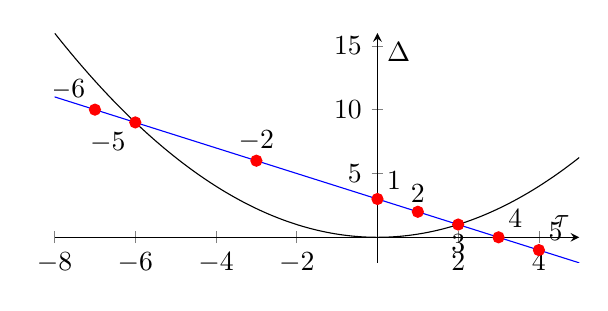
\begin{tikzpicture}\begin{axis}[width=.68\textwidth,height=4.5cm,axis lines=middle,xlabel={$\tau$},ylabel={$\Delta$},samples=130,xmin=-8,xmax=5,ymin=-2,ymax=16]
\addplot[black,domain=-8:5]{x*x/4};\addplot[blue,domain=-8:5]{3-x};\addplot[only marks,red] coordinates{(-7,10)(-6,9)(-3,6)(0,3)(1,2)(2,1)(3,0)(4,-1)};\node[above left] at(axis cs:-7,10){$-6$};\node[below left] at(axis cs:-6,9){$-5$};\node[above] at(axis cs:-3,6){$-2$};\node[above right] at(axis cs:0,3){$1$};\node[above] at(axis cs:1,2){$2$};\node[below] at(axis cs:2,1){$3$};\node[above right] at(axis cs:3,0){$4$};\node[above right] at(axis cs:4,-1){$5$};\end{axis}\end{tikzpicture}\end{center}
\par\noindent{\small 依据：官方译审并补证（AI辅助）。}
\end{solution}

\begin{exercise}\label{cw:rec23-3}
对上述八个$a$列出：(1)特征值；(2)由特征值确定的相图种类及稳定类型：所有实部负称稳定，至少一个实部正称不稳定，否则不指定；(3)额外信息：螺旋的旋转方向，重根是否亏损。每例画小相图，传达分类即可，不要求猜准特征方向。
\end{exercise}
\begin{solution}
计算结果如下；“不指定”沿用本题措辞，中心实际为中性稳定。
\[\begin{array}{c|c|l}
a&\text{特征值}&\text{相图与稳定类型}\\\hline
-6&-5,-2&\text{稳定结点}\\
-5&-3,-3&\text{亏损稳定结点}\\
-2&(-3\pm\ii\sqrt{15})/2&\text{顺时针稳定螺旋}\\
1&\pm\ii\sqrt3&\text{顺时针中心；不指定}\\
2&(1\pm\ii\sqrt7)/2&\text{顺时针不稳定螺旋}\\
3&1,1&\text{亏损不稳定结点}\\
4&0,3&\text{一条平衡线与不稳定横向运动}\\
5&2\pm\sqrt5&\text{鞍点；不稳定}
\end{array}\]
非实根情形，在正$x$轴速度的$y$分量为$-2x<0$，故顺时针。重根处$A-\lambda I\ne0$且平方为0，所以只有一条特征方向，均亏损。$a=4$不是孤立结点：零特征空间由平衡点构成。以下用实际矩阵指数计算坐标重绘，相图类别由上述解析结果确定。\begin{center}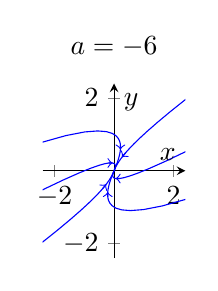
\begin{tikzpicture}\begin{axis}[width=.28\textwidth,height=3.8cm,axis lines=middle,title={$a=-6$},xlabel={$x$},ylabel={$y$},xmin=-2.4,xmax=2.4,ymin=-2.4,ymax=2.4,clip=true]\addplot[blue,no marks] coordinates {(2.47250,0.55125) (1.71722,0.25689) (1.17962,0.06125) (0.79840,-0.06510) (0.52935,-0.14318) (0.34062,-0.18796) (0.20926,-0.21008) (0.11877,-0.21706) (0.05729,-0.21419) (0.01630,-0.20516) (-0.01029,-0.19252) (-0.02683,-0.17801) (-0.03644,-0.16280) (-0.04131,-0.14766) (-0.04302,-0.13307) (-0.04266,-0.11933) (-0.04099,-0.10658) (-0.03855,-0.09490) (-0.03571,-0.08428) (-0.03270,-0.07470) (-0.02968,-0.06610) (-0.02677,-0.05841) (-0.02402,-0.05156) (-0.02146,-0.04547) (-0.01912,-0.04008) (-0.01698,-0.03530) (-0.01506,-0.03108) (-0.01333,-0.02735) (-0.01178,-0.02406) (-0.01040,-0.02116) (-0.00917,-0.01861) (-0.00808,-0.01636) (-0.00712,-0.01438) (-0.00627,-0.01264) (-0.00552,-0.01111) (-0.00485,-0.00976) (-0.00427,-0.00858) (-0.00375,-0.00754) (-0.00330,-0.00662) (-0.00290,-0.00582) (-0.00255,-0.00511) (-0.00224,-0.00449)};\draw[blue,->] (axis cs:0.17983,-0.21335)--(axis cs:0.05061,-0.21325);\addplot[blue,no marks] coordinates {(-2.47250,-0.55125) (-1.71722,-0.25689) (-1.17962,-0.06125) (-0.79840,0.06510) (-0.52935,0.14318) (-0.34062,0.18796) (-0.20926,0.21008) (-0.11877,0.21706) (-0.05729,0.21419) (-0.01630,0.20516) (0.01029,0.19252) (0.02683,0.17801) (0.03644,0.16280) (0.04131,0.14766) (0.04302,0.13307) (0.04266,0.11933) (0.04099,0.10658) (0.03855,0.09490) (0.03571,0.08428) (0.03270,0.07470) (0.02968,0.06610) (0.02677,0.05841) (0.02402,0.05156) (0.02146,0.04547) (0.01912,0.04008) (0.01698,0.03530) (0.01506,0.03108) (0.01333,0.02735) (0.01178,0.02406) (0.01040,0.02116) (0.00917,0.01861) (0.00808,0.01636) (0.00712,0.01438) (0.00627,0.01264) (0.00552,0.01111) (0.00485,0.00976) (0.00427,0.00858) (0.00375,0.00754) (0.00330,0.00662) (0.00290,0.00582) (0.00255,0.00511) (0.00224,0.00449)};\draw[blue,->] (axis cs:-0.17983,0.21335)--(axis cs:-0.05061,0.21325);\addplot[blue,no marks] coordinates {(-2.52461,0.75892) (-1.61662,0.96717) (-0.98541,1.06692) (-0.55125,1.09438) (-0.25689,1.07500) (-0.06125,1.02650) (0.06510,0.96115) (0.14318,0.88729) (0.18796,0.81051) (0.21008,0.73445) (0.21706,0.66142) (0.21419,0.59277) (0.20516,0.52921) (0.19252,0.47102) (0.17801,0.41820) (0.16280,0.37057) (0.14766,0.32784) (0.13307,0.28967) (0.11933,0.25567) (0.10658,0.22546) (0.09490,0.19869) (0.08428,0.17499) (0.07470,0.15405) (0.06610,0.13556) (0.05841,0.11925) (0.05156,0.10488) (0.04547,0.09222) (0.04008,0.08107) (0.03530,0.07126) (0.03108,0.06263) (0.02735,0.05504) (0.02406,0.04837) (0.02116,0.04250) (0.01861,0.03734) (0.01636,0.03281) (0.01438,0.02883) (0.01264,0.02533) (0.01111,0.02225) (0.00976,0.01955) (0.00858,0.01717) (0.00754,0.01508) (0.00662,0.01325) (0.00582,0.01164) (0.00511,0.01023) (0.00449,0.00898)};\draw[blue,->] (axis cs:0.21335,0.71321)--(axis cs:0.21325,0.58374);\addplot[blue,no marks] coordinates {(2.52461,-0.75892) (1.61662,-0.96717) (0.98541,-1.06692) (0.55125,-1.09438) (0.25689,-1.07500) (0.06125,-1.02650) (-0.06510,-0.96115) (-0.14318,-0.88729) (-0.18796,-0.81051) (-0.21008,-0.73445) (-0.21706,-0.66142) (-0.21419,-0.59277) (-0.20516,-0.52921) (-0.19252,-0.47102) (-0.17801,-0.41820) (-0.16280,-0.37057) (-0.14766,-0.32784) (-0.13307,-0.28967) (-0.11933,-0.25567) (-0.10658,-0.22546) (-0.09490,-0.19869) (-0.08428,-0.17499) (-0.07470,-0.15405) (-0.06610,-0.13556) (-0.05841,-0.11925) (-0.05156,-0.10488) (-0.04547,-0.09222) (-0.04008,-0.08107) (-0.03530,-0.07126) (-0.03108,-0.06263) (-0.02735,-0.05504) (-0.02406,-0.04837) (-0.02116,-0.04250) (-0.01861,-0.03734) (-0.01636,-0.03281) (-0.01438,-0.02883) (-0.01264,-0.02533) (-0.01111,-0.02225) (-0.00976,-0.01955) (-0.00858,-0.01717) (-0.00754,-0.01508) (-0.00662,-0.01325) (-0.00582,-0.01164) (-0.00511,-0.01023) (-0.00449,-0.00898)};\draw[blue,->] (axis cs:-0.21335,-0.71321)--(axis cs:-0.21325,-0.58374);\addplot[blue,no marks] coordinates {(3.39211,2.58380) (2.54503,2.05233) (1.92125,1.64563) (1.46033,1.33189) (1.11837,1.08775) (0.86350,0.89605) (0.67253,0.74412) (0.52858,0.62255) (0.41934,0.52438) (0.33583,0.44436) (0.27148,0.37858) (0.22146,0.32404) (0.18223,0.27850) (0.15118,0.24019) (0.12637,0.20777) (0.10635,0.18018) (0.09006,0.15659) (0.07667,0.13634) (0.06559,0.11888) (0.05634,0.10379) (0.04857,0.09071) (0.04200,0.07935) (0.03641,0.06946) (0.03164,0.06084) (0.02754,0.05332) (0.02401,0.04675) (0.02096,0.04100) (0.01832,0.03597) (0.01602,0.03156) (0.01402,0.02770) (0.01228,0.02431) (0.01076,0.02134) (0.00943,0.01874) (0.00827,0.01645) (0.00726,0.01445) (0.00637,0.01269) (0.00559,0.01114) (0.00491,0.00979) (0.00431,0.00859) (0.00378,0.00755) (0.00332,0.00663) (0.00292,0.00582) (0.00256,0.00512) (0.00225,0.00449)};\draw[blue,->] (axis cs:0.39318,0.49986)--(axis cs:0.26386,0.37049);\addplot[blue,no marks] coordinates {(-3.39211,-2.58380) (-2.54503,-2.05233) (-1.92125,-1.64563) (-1.46033,-1.33189) (-1.11837,-1.08775) (-0.86350,-0.89605) (-0.67253,-0.74412) (-0.52858,-0.62255) (-0.41934,-0.52438) (-0.33583,-0.44436) (-0.27148,-0.37858) (-0.22146,-0.32404) (-0.18223,-0.27850) (-0.15118,-0.24019) (-0.12637,-0.20777) (-0.10635,-0.18018) (-0.09006,-0.15659) (-0.07667,-0.13634) (-0.06559,-0.11888) (-0.05634,-0.10379) (-0.04857,-0.09071) (-0.04200,-0.07935) (-0.03641,-0.06946) (-0.03164,-0.06084) (-0.02754,-0.05332) (-0.02401,-0.04675) (-0.02096,-0.04100) (-0.01832,-0.03597) (-0.01602,-0.03156) (-0.01402,-0.02770) (-0.01228,-0.02431) (-0.01076,-0.02134) (-0.00943,-0.01874) (-0.00827,-0.01645) (-0.00726,-0.01445) (-0.00637,-0.01269) (-0.00559,-0.01114) (-0.00491,-0.00979) (-0.00431,-0.00859) (-0.00378,-0.00755) (-0.00332,-0.00663) (-0.00292,-0.00582) (-0.00256,-0.00512) (-0.00225,-0.00449)};\draw[blue,->] (axis cs:-0.39318,-0.49986)--(axis cs:-0.26386,-0.37049);\end{axis}\end{tikzpicture}\hspace{.035\textwidth}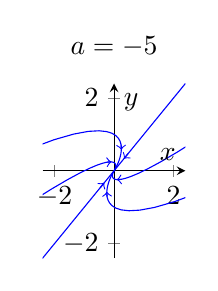
\begin{tikzpicture}\begin{axis}[width=.28\textwidth,height=3.8cm,axis lines=middle,title={$a=-5$},xlabel={$x$},ylabel={$y$},xmin=-2.4,xmax=2.4,ymin=-2.4,ymax=2.4,clip=true]\addplot[blue,no marks] coordinates {(2.81339,0.86566) (2.10838,0.50482) (1.56467,0.24448) (1.14729,0.06038) (0.82855,-0.06628) (0.58664,-0.15007) (0.40435,-0.20218) (0.26817,-0.23118) (0.16749,-0.24362) (0.09402,-0.24445) (0.04128,-0.23737) (0.00425,-0.22517) (-0.02099,-0.20986) (-0.03744,-0.19293) (-0.04742,-0.17544) (-0.05270,-0.15810) (-0.05464,-0.14141) (-0.05424,-0.12568) (-0.05228,-0.11110) (-0.04932,-0.09774) (-0.04577,-0.08564) (-0.04194,-0.07476) (-0.03803,-0.06505) (-0.03419,-0.05644) (-0.03053,-0.04884) (-0.02709,-0.04217) (-0.02391,-0.03632) (-0.02101,-0.03123) (-0.01839,-0.02680) (-0.01604,-0.02296) (-0.01394,-0.01965) (-0.01209,-0.01678) (-0.01045,-0.01432) (-0.00902,-0.01220) (-0.00776,-0.01038) (-0.00667,-0.00883) (-0.00572,-0.00750) (-0.00490,-0.00636) (-0.00419,-0.00540) (-0.00358,-0.00457) (-0.00305,-0.00387) (-0.00260,-0.00327) (-0.00221,-0.00277)};\draw[blue,->] (axis cs:0.23618,-0.23618)--(axis cs:0.08569,-0.24387);\addplot[blue,no marks] coordinates {(-2.81339,-0.86566) (-2.10838,-0.50482) (-1.56467,-0.24448) (-1.14729,-0.06038) (-0.82855,0.06628) (-0.58664,0.15007) (-0.40435,0.20218) (-0.26817,0.23118) (-0.16749,0.24362) (-0.09402,0.24445) (-0.04128,0.23737) (-0.00425,0.22517) (0.02099,0.20986) (0.03744,0.19293) (0.04742,0.17544) (0.05270,0.15810) (0.05464,0.14141) (0.05424,0.12568) (0.05228,0.11110) (0.04932,0.09774) (0.04577,0.08564) (0.04194,0.07476) (0.03803,0.06505) (0.03419,0.05644) (0.03053,0.04884) (0.02709,0.04217) (0.02391,0.03632) (0.02101,0.03123) (0.01839,0.02680) (0.01604,0.02296) (0.01394,0.01965) (0.01209,0.01678) (0.01045,0.01432) (0.00902,0.01220) (0.00776,0.01038) (0.00667,0.00883) (0.00572,0.00750) (0.00490,0.00636) (0.00419,0.00540) (0.00358,0.00457) (0.00305,0.00387) (0.00260,0.00327) (0.00221,0.00277)};\draw[blue,->] (axis cs:-0.23618,0.23618)--(axis cs:-0.08569,0.24387);\addplot[blue,no marks] coordinates {(-2.90862,0.58172) (-2.02214,0.85143) (-1.35814,1.00765) (-0.86566,1.08207) (-0.50482,1.09873) (-0.24448,1.07571) (-0.06038,1.02652) (0.06628,0.96112) (0.15007,0.88679) (0.20218,0.80871) (0.23118,0.73053) (0.24362,0.65473) (0.24445,0.58291) (0.23737,0.51603) (0.22517,0.45458) (0.20986,0.39874) (0.19293,0.34843) (0.17544,0.30346) (0.15810,0.26350) (0.14141,0.22818) (0.12568,0.19712) (0.11110,0.16991) (0.09774,0.14617) (0.08564,0.12551) (0.07476,0.10758) (0.06505,0.09207) (0.05644,0.07869) (0.04884,0.06716) (0.04217,0.05724) (0.03632,0.04874) (0.03123,0.04145) (0.02680,0.03522) (0.02296,0.02989) (0.01965,0.02535) (0.01678,0.02148) (0.01432,0.01818) (0.01220,0.01538) (0.01038,0.01300) (0.00883,0.01099) (0.00750,0.00928) (0.00636,0.00783) (0.00540,0.00660) (0.00457,0.00556) (0.00387,0.00468) (0.00327,0.00394) (0.00277,0.00332)};\draw[blue,->] (axis cs:0.23618,0.70855)--(axis cs:0.24387,0.57343);\addplot[blue,no marks] coordinates {(2.90862,-0.58172) (2.02214,-0.85143) (1.35814,-1.00765) (0.86566,-1.08207) (0.50482,-1.09873) (0.24448,-1.07571) (0.06038,-1.02652) (-0.06628,-0.96112) (-0.15007,-0.88679) (-0.20218,-0.80871) (-0.23118,-0.73053) (-0.24362,-0.65473) (-0.24445,-0.58291) (-0.23737,-0.51603) (-0.22517,-0.45458) (-0.20986,-0.39874) (-0.19293,-0.34843) (-0.17544,-0.30346) (-0.15810,-0.26350) (-0.14141,-0.22818) (-0.12568,-0.19712) (-0.11110,-0.16991) (-0.09774,-0.14617) (-0.08564,-0.12551) (-0.07476,-0.10758) (-0.06505,-0.09207) (-0.05644,-0.07869) (-0.04884,-0.06716) (-0.04217,-0.05724) (-0.03632,-0.04874) (-0.03123,-0.04145) (-0.02680,-0.03522) (-0.02296,-0.02989) (-0.01965,-0.02535) (-0.01678,-0.02148) (-0.01432,-0.01818) (-0.01220,-0.01538) (-0.01038,-0.01300) (-0.00883,-0.01099) (-0.00750,-0.00928) (-0.00636,-0.00783) (-0.00540,-0.00660) (-0.00457,-0.00556) (-0.00387,-0.00468) (-0.00327,-0.00394) (-0.00277,-0.00332)};\draw[blue,->] (axis cs:-0.23618,-0.70855)--(axis cs:-0.24387,-0.57343);\addplot[blue,no marks] coordinates {(3.49034,3.49034) (2.87357,2.87357) (2.36579,2.36579) (1.94773,1.94773) (1.60355,1.60355) (1.32019,1.32019) (1.08690,1.08690) (0.89484,0.89484) (0.73671,0.73671) (0.60653,0.60653) (0.49935,0.49935) (0.41111,0.41111) (0.33847,0.33847) (0.27866,0.27866) (0.22942,0.22942) (0.18888,0.18888) (0.15550,0.15550) (0.12802,0.12802) (0.10540,0.10540) (0.08677,0.08677) (0.07144,0.07144) (0.05882,0.05882) (0.04842,0.04842) (0.03987,0.03987) (0.03282,0.03282) (0.02702,0.02702) (0.02225,0.02225) (0.01832,0.01832) (0.01508,0.01508) (0.01241,0.01241) (0.01022,0.01022) (0.00841,0.00841) (0.00693,0.00693) (0.00570,0.00570) (0.00470,0.00470) (0.00387,0.00387) (0.00318,0.00318) (0.00262,0.00262) (0.00216,0.00216) (0.00178,0.00178) (0.00146,0.00146) (0.00120,0.00120) (0.00099,0.00099) (0.00082,0.00082) (0.00067,0.00067) (0.00055,0.00055)};\draw[blue,->] (axis cs:0.47237,0.47237)--(axis cs:0.32956,0.32956);\addplot[blue,no marks] coordinates {(-3.49034,-3.49034) (-2.87357,-2.87357) (-2.36579,-2.36579) (-1.94773,-1.94773) (-1.60355,-1.60355) (-1.32019,-1.32019) (-1.08690,-1.08690) (-0.89484,-0.89484) (-0.73671,-0.73671) (-0.60653,-0.60653) (-0.49935,-0.49935) (-0.41111,-0.41111) (-0.33847,-0.33847) (-0.27866,-0.27866) (-0.22942,-0.22942) (-0.18888,-0.18888) (-0.15550,-0.15550) (-0.12802,-0.12802) (-0.10540,-0.10540) (-0.08677,-0.08677) (-0.07144,-0.07144) (-0.05882,-0.05882) (-0.04842,-0.04842) (-0.03987,-0.03987) (-0.03282,-0.03282) (-0.02702,-0.02702) (-0.02225,-0.02225) (-0.01832,-0.01832) (-0.01508,-0.01508) (-0.01241,-0.01241) (-0.01022,-0.01022) (-0.00841,-0.00841) (-0.00693,-0.00693) (-0.00570,-0.00570) (-0.00470,-0.00470) (-0.00387,-0.00387) (-0.00318,-0.00318) (-0.00262,-0.00262) (-0.00216,-0.00216) (-0.00178,-0.00178) (-0.00146,-0.00146) (-0.00120,-0.00120) (-0.00099,-0.00099) (-0.00082,-0.00082) (-0.00067,-0.00067) (-0.00055,-0.00055)};\draw[blue,->] (axis cs:-0.47237,-0.47237)--(axis cs:-0.32956,-0.32956);\end{axis}\end{tikzpicture}\hspace{.035\textwidth}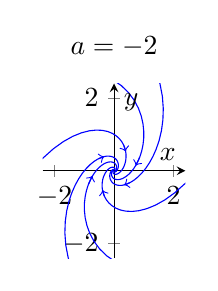
\begin{tikzpicture}\begin{axis}[width=.28\textwidth,height=3.8cm,axis lines=middle,title={$a=-2$},xlabel={$x$},ylabel={$y$},xmin=-2.4,xmax=2.4,ymin=-2.4,ymax=2.4,clip=true]\addplot[blue,no marks] coordinates {(0.90068,3.45749) (1.19000,3.10823) (1.40098,2.74964) (1.54267,2.39156) (1.62405,2.04209) (1.65393,1.70770) (1.64072,1.39335) (1.59234,1.10271) (1.51611,0.83822) (1.41870,0.60130) (1.30607,0.39251) (1.18349,0.21164) (1.05551,0.05789) (0.92602,-0.07001) (0.79825,-0.17371) (0.67481,-0.25512) (0.55776,-0.31631) (0.44864,-0.35945) (0.34855,-0.38676) (0.25817,-0.40040) (0.17787,-0.40247) (0.10769,-0.39498) (0.04745,-0.37979) (-0.00323,-0.35859) (-0.04488,-0.33295) (-0.07814,-0.30423) (-0.10374,-0.27363) (-0.12245,-0.24218) (-0.13505,-0.21075) (-0.14234,-0.18006) (-0.14508,-0.15067) (-0.14403,-0.12304) (-0.13987,-0.09747) (-0.13324,-0.07420) (-0.12474,-0.05334) (-0.11489,-0.03495) (-0.10416,-0.01901) (-0.09294,-0.00545) (-0.08158,0.00584) (-0.07036,0.01500) (-0.05952,0.02219) (-0.04923,0.02761) (-0.03964,0.03144) (-0.03083,0.03388) (-0.02287,0.03511) (-0.01580,0.03532) (-0.00962,0.03468) (-0.00431,0.03337) (0.00016,0.03152) (0.00384,0.02928) (0.00678,0.02677) (0.00904,0.02409)};\draw[blue,->] (axis cs:0.52571,-0.33038)--(axis cs:0.33557,-0.38939);\addplot[blue,no marks] coordinates {(-0.90068,-3.45749) (-1.19000,-3.10823) (-1.40098,-2.74964) (-1.54267,-2.39156) (-1.62405,-2.04209) (-1.65393,-1.70770) (-1.64072,-1.39335) (-1.59234,-1.10271) (-1.51611,-0.83822) (-1.41870,-0.60130) (-1.30607,-0.39251) (-1.18349,-0.21164) (-1.05551,-0.05789) (-0.92602,0.07001) (-0.79825,0.17371) (-0.67481,0.25512) (-0.55776,0.31631) (-0.44864,0.35945) (-0.34855,0.38676) (-0.25817,0.40040) (-0.17787,0.40247) (-0.10769,0.39498) (-0.04745,0.37979) (0.00323,0.35859) (0.04488,0.33295) (0.07814,0.30423) (0.10374,0.27363) (0.12245,0.24218) (0.13505,0.21075) (0.14234,0.18006) (0.14508,0.15067) (0.14403,0.12304) (0.13987,0.09747) (0.13324,0.07420) (0.12474,0.05334) (0.11489,0.03495) (0.10416,0.01901) (0.09294,0.00545) (0.08158,-0.00584) (0.07036,-0.01500) (0.05952,-0.02219) (0.04923,-0.02761) (0.03964,-0.03144) (0.03083,-0.03388) (0.02287,-0.03511) (0.01580,-0.03532) (0.00962,-0.03468) (0.00431,-0.03337) (-0.00016,-0.03152) (-0.00384,-0.02928) (-0.00678,-0.02677) (-0.00904,-0.02409)};\draw[blue,->] (axis cs:-0.52571,0.33038)--(axis cs:-0.33557,0.38939);\addplot[blue,no marks] coordinates {(-3.45749,-0.82807) (-3.10823,-0.36412) (-2.74964,0.02616) (-2.39156,0.34689) (-2.04209,0.60300) (-1.70770,0.80008) (-1.39335,0.94404) (-1.10271,1.04098) (-0.83822,1.09700) (-0.60130,1.11804) (-0.39251,1.10981) (-0.21164,1.07767) (-0.05789,1.02657) (0.07001,0.96103) (0.17371,0.88511) (0.25512,0.80237) (0.31631,0.71591) (0.35945,0.62836) (0.38676,0.54192) (0.40040,0.45837) (0.40247,0.37911) (0.39498,0.30518) (0.37979,0.23734) (0.35859,0.17607) (0.33295,0.12160) (0.30423,0.07397) (0.27363,0.03307) (0.24218,-0.00136) (0.21075,-0.02967) (0.18006,-0.05231) (0.15067,-0.06975) (0.12304,-0.08251) (0.09747,-0.09113) (0.07420,-0.09614) (0.05334,-0.09807) (0.03495,-0.09742) (0.01901,-0.09466) (0.00545,-0.09022) (-0.00584,-0.08450) (-0.01500,-0.07786) (-0.02219,-0.07062) (-0.02761,-0.06304) (-0.03144,-0.05536) (-0.03388,-0.04777) (-0.03511,-0.04043) (-0.03532,-0.03346) (-0.03468,-0.02696) (-0.03337,-0.02099) (-0.03152,-0.01560) (-0.02928,-0.01080) (-0.02677,-0.00661) (-0.02409,-0.00300)};\draw[blue,->] (axis cs:0.33038,0.69090)--(axis cs:0.38939,0.53026);\addplot[blue,no marks] coordinates {(3.45749,0.82807) (3.10823,0.36412) (2.74964,-0.02616) (2.39156,-0.34689) (2.04209,-0.60300) (1.70770,-0.80008) (1.39335,-0.94404) (1.10271,-1.04098) (0.83822,-1.09700) (0.60130,-1.11804) (0.39251,-1.10981) (0.21164,-1.07767) (0.05789,-1.02657) (-0.07001,-0.96103) (-0.17371,-0.88511) (-0.25512,-0.80237) (-0.31631,-0.71591) (-0.35945,-0.62836) (-0.38676,-0.54192) (-0.40040,-0.45837) (-0.40247,-0.37911) (-0.39498,-0.30518) (-0.37979,-0.23734) (-0.35859,-0.17607) (-0.33295,-0.12160) (-0.30423,-0.07397) (-0.27363,-0.03307) (-0.24218,0.00136) (-0.21075,0.02967) (-0.18006,0.05231) (-0.15067,0.06975) (-0.12304,0.08251) (-0.09747,0.09113) (-0.07420,0.09614) (-0.05334,0.09807) (-0.03495,0.09742) (-0.01901,0.09466) (-0.00545,0.09022) (0.00584,0.08450) (0.01500,0.07786) (0.02219,0.07062) (0.02761,0.06304) (0.03144,0.05536) (0.03388,0.04777) (0.03511,0.04043) (0.03532,0.03346) (0.03468,0.02696) (0.03337,0.02099) (0.03152,0.01560) (0.02928,0.01080) (0.02677,0.00661) (0.02409,0.00300)};\draw[blue,->] (axis cs:-0.33038,-0.69090)--(axis cs:-0.38939,-0.53026);\addplot[blue,no marks] coordinates {(-3.26146,2.41712) (-2.55681,2.62943) (-1.91824,2.74411) (-1.34866,2.77581) (-0.84890,2.73845) (-0.41804,2.64509) (-0.05377,2.50777) (0.24736,2.33740) (0.48963,2.14369) (0.67789,1.93522) (0.81739,1.71935) (0.91356,1.50232) (0.97185,1.28930) (0.99762,1.08446) (0.99604,0.89102) (0.97196,0.71140) (0.92993,0.54725) (0.87406,0.39960) (0.80809,0.26891) (0.73530,0.15517) (0.65857,0.05798) (0.58034,-0.02337) (0.50267,-0.08980) (0.42724,-0.14244) (0.35537,-0.18253) (0.28807,-0.21136) (0.22608,-0.23026) (0.16988,-0.24056) (0.11973,-0.24354) (0.07570,-0.24042) (0.03772,-0.23237) (0.00559,-0.22042) (-0.02099,-0.20555) (-0.04239,-0.18860) (-0.05904,-0.17034) (-0.07140,-0.15141) (-0.07995,-0.13237) (-0.08515,-0.11366) (-0.08749,-0.09567) (-0.08742,-0.07866) (-0.08536,-0.06287) (-0.08171,-0.04842) (-0.07684,-0.03542) (-0.07108,-0.02391) (-0.06471,-0.01389) (-0.05798,-0.00532) (-0.05112,0.00186) (-0.04430,0.00772) (-0.03768,0.01238) (-0.03136,0.01592) (-0.02544,0.01848) (-0.01999,0.02016) (-0.01504,0.02109)};\draw[blue,->] (axis cs:0.85609,0.36053)--(axis cs:0.72495,0.14087);\addplot[blue,no marks] coordinates {(3.26146,-2.41712) (2.55681,-2.62943) (1.91824,-2.74411) (1.34866,-2.77581) (0.84890,-2.73845) (0.41804,-2.64509) (0.05377,-2.50777) (-0.24736,-2.33740) (-0.48963,-2.14369) (-0.67789,-1.93522) (-0.81739,-1.71935) (-0.91356,-1.50232) (-0.97185,-1.28930) (-0.99762,-1.08446) (-0.99604,-0.89102) (-0.97196,-0.71140) (-0.92993,-0.54725) (-0.87406,-0.39960) (-0.80809,-0.26891) (-0.73530,-0.15517) (-0.65857,-0.05798) (-0.58034,0.02337) (-0.50267,0.08980) (-0.42724,0.14244) (-0.35537,0.18253) (-0.28807,0.21136) (-0.22608,0.23026) (-0.16988,0.24056) (-0.11973,0.24354) (-0.07570,0.24042) (-0.03772,0.23237) (-0.00559,0.22042) (0.02099,0.20555) (0.04239,0.18860) (0.05904,0.17034) (0.07140,0.15141) (0.07995,0.13237) (0.08515,0.11366) (0.08749,0.09567) (0.08742,0.07866) (0.08536,0.06287) (0.08171,0.04842) (0.07684,0.03542) (0.07108,0.02391) (0.06471,0.01389) (0.05798,0.00532) (0.05112,-0.00186) (0.04430,-0.00772) (0.03768,-0.01238) (0.03136,-0.01592) (0.02544,-0.01848) (0.01999,-0.02016) (0.01504,-0.02109)};\draw[blue,->] (axis cs:-0.85609,-0.36053)--(axis cs:-0.72495,-0.14087);\end{axis}\end{tikzpicture}\par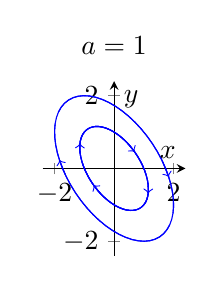
\begin{tikzpicture}\begin{axis}[width=.28\textwidth,height=3.8cm,axis lines=middle,title={$a=1$},xlabel={$x$},ylabel={$y$},xmin=-2.4,xmax=2.4,ymin=-2.4,ymax=2.4,clip=true]\addplot[blue,no marks] coordinates {(-0.73042,1.13972) (-0.62563,1.15332) (-0.51297,1.15239) (-0.39385,1.13696) (-0.26977,1.10721) (-0.14229,1.06352) (-0.01302,1.00645) (0.11641,0.93670) (0.24437,0.85516) (0.36926,0.76286) (0.48950,0.66095) (0.60358,0.55072) (0.71006,0.43355) (0.80760,0.31093) (0.89497,0.18439) (0.97108,0.05553) (1.03495,-0.07402) (1.08580,-0.20265) (1.12298,-0.32872) (1.14602,-0.45066) (1.15464,-0.56692) (1.14871,-0.67605) (1.12833,-0.77666) (1.09374,-0.86749) (1.04538,-0.94741) (0.98386,-1.01540) (0.90995,-1.07060) (0.82459,-1.11232) (0.72884,-1.14004) (0.62392,-1.15341) (0.51115,-1.15226) (0.39194,-1.13660) (0.26779,-1.10663) (0.14027,-1.06273) (0.01099,-1.00545) (-0.11843,-0.93551) (-0.24636,-0.85380) (-0.37119,-0.76133) (-0.49134,-0.65928) (-0.60531,-0.54893) (-0.71166,-0.43167) (-0.80905,-0.30897) (-0.89625,-0.18239) (-0.97217,-0.05351) (-1.03585,0.07605) (-1.08649,0.20465) (-1.12345,0.33067) (-1.14627,0.45253) (-1.15466,0.56869) (-1.14851,0.67769) (-1.12790,0.77816) (-1.09309,0.86883) (-1.04452,0.94857) (-0.98279,1.01636) (-0.90870,1.07136)};\draw[blue,->] (axis cs:1.14997,-0.48452)--(axis cs:1.14677,-0.69038);\addplot[blue,no marks] coordinates {(0.73042,-1.13972) (0.62563,-1.15332) (0.51297,-1.15239) (0.39385,-1.13696) (0.26977,-1.10721) (0.14229,-1.06352) (0.01302,-1.00645) (-0.11641,-0.93670) (-0.24437,-0.85516) (-0.36926,-0.76286) (-0.48950,-0.66095) (-0.60358,-0.55072) (-0.71006,-0.43355) (-0.80760,-0.31093) (-0.89497,-0.18439) (-0.97108,-0.05553) (-1.03495,0.07402) (-1.08580,0.20265) (-1.12298,0.32872) (-1.14602,0.45066) (-1.15464,0.56692) (-1.14871,0.67605) (-1.12833,0.77666) (-1.09374,0.86749) (-1.04538,0.94741) (-0.98386,1.01540) (-0.90995,1.07060) (-0.82459,1.11232) (-0.72884,1.14004) (-0.62392,1.15341) (-0.51115,1.15226) (-0.39194,1.13660) (-0.26779,1.10663) (-0.14027,1.06273) (-0.01099,1.00545) (0.11843,0.93551) (0.24636,0.85380) (0.37119,0.76133) (0.49134,0.65928) (0.60531,0.54893) (0.71166,0.43167) (0.80905,0.30897) (0.89625,0.18239) (0.97217,0.05351) (1.03585,-0.07605) (1.08649,-0.20465) (1.12345,-0.33067) (1.14627,-0.45253) (1.15466,-0.56869) (1.14851,-0.67769) (1.12790,-0.77816) (1.09309,-0.86883) (1.04452,-0.94857) (0.98279,-1.01636) (0.90870,-1.07136)};\draw[blue,->] (axis cs:-1.14997,0.48452)--(axis cs:-1.14677,0.69038);\addplot[blue,no marks] coordinates {(-1.13972,0.40930) (-1.15332,0.52769) (-1.15239,0.63942) (-1.13696,0.74311) (-1.10721,0.83744) (-1.06352,0.92123) (-1.00645,0.99343) (-0.93670,1.05311) (-0.85516,1.09954) (-0.76286,1.13212) (-0.66095,1.15045) (-0.55072,1.15430) (-0.43355,1.14361) (-0.31093,1.11853) (-0.18439,1.07936) (-0.05553,1.02661) (0.07402,0.96093) (0.20265,0.88316) (0.32872,0.79426) (0.45066,0.69537) (0.56692,0.58772) (0.67605,0.47267) (0.77666,0.35167) (0.86749,0.22624) (0.94741,0.09797) (1.01540,-0.03154) (1.07060,-0.16065) (1.11232,-0.28774) (1.14004,-0.41120) (1.15341,-0.52949) (1.15226,-0.64111) (1.13660,-0.74466) (1.10663,-0.83884) (1.06273,-0.92246) (1.00545,-0.99446) (0.93551,-1.05394) (0.85380,-1.10015) (0.76133,-1.13252) (0.65928,-1.15062) (0.54893,-1.15424) (0.43167,-1.14333) (0.30897,-1.11802) (0.18239,-1.07864) (0.05351,-1.02568) (-0.07605,-0.95980) (-0.20465,-0.88185) (-0.33067,-0.79279) (-0.45253,-0.69374) (-0.56869,-0.58597) (-0.67769,-0.47082) (-0.77816,-0.34974) (-0.86883,-0.22425) (-0.94857,-0.09595) (-1.01636,0.03357) (-1.07136,0.16266)};\draw[blue,->] (axis cs:0.48452,0.66545)--(axis cs:0.69038,0.45639);\addplot[blue,no marks] coordinates {(1.13972,-0.40930) (1.15332,-0.52769) (1.15239,-0.63942) (1.13696,-0.74311) (1.10721,-0.83744) (1.06352,-0.92123) (1.00645,-0.99343) (0.93670,-1.05311) (0.85516,-1.09954) (0.76286,-1.13212) (0.66095,-1.15045) (0.55072,-1.15430) (0.43355,-1.14361) (0.31093,-1.11853) (0.18439,-1.07936) (0.05553,-1.02661) (-0.07402,-0.96093) (-0.20265,-0.88316) (-0.32872,-0.79426) (-0.45066,-0.69537) (-0.56692,-0.58772) (-0.67605,-0.47267) (-0.77666,-0.35167) (-0.86749,-0.22624) (-0.94741,-0.09797) (-1.01540,0.03154) (-1.07060,0.16065) (-1.11232,0.28774) (-1.14004,0.41120) (-1.15341,0.52949) (-1.15226,0.64111) (-1.13660,0.74466) (-1.10663,0.83884) (-1.06273,0.92246) (-1.00545,0.99446) (-0.93551,1.05394) (-0.85380,1.10015) (-0.76133,1.13252) (-0.65928,1.15062) (-0.54893,1.15424) (-0.43167,1.14333) (-0.30897,1.11802) (-0.18239,1.07864) (-0.05351,1.02568) (0.07605,0.95980) (0.20465,0.88185) (0.33067,0.79279) (0.45253,0.69374) (0.56869,0.58597) (0.67769,0.47082) (0.77816,0.34974) (0.86883,0.22425) (0.94857,0.09595) (1.01636,-0.03357) (1.07136,-0.16266)};\draw[blue,->] (axis cs:-0.48452,-0.66545)--(axis cs:-0.69038,-0.45639);\addplot[blue,no marks] coordinates {(-1.87014,1.54902) (-1.77894,1.68100) (-1.66536,1.79181) (-1.53080,1.88007) (-1.37698,1.94465) (-1.20581,1.98476) (-1.01947,1.99987) (-0.82029,1.98981) (-0.61079,1.95470) (-0.39359,1.89498) (-0.17144,1.81140) (0.05287,1.70501) (0.27651,1.57716) (0.49667,1.42946) (0.71058,1.26376) (0.91554,1.08214) (1.10898,0.88691) (1.28845,0.68051) (1.45171,0.46554) (1.59668,0.24471) (1.72156,0.02080) (1.82476,-0.20338) (1.90499,-0.42499) (1.96123,-0.64125) (1.99279,-0.84944) (1.99925,-1.04693) (1.98055,-1.23125) (1.93691,-1.40006) (1.86889,-1.55125) (1.77733,-1.68290) (1.66341,-1.79337) (1.52854,-1.88127) (1.37442,-1.94547) (1.20300,-1.98519) (1.01644,-1.99991) (0.81708,-1.98945) (0.60744,-1.95395) (0.39014,-1.89385) (0.16794,-1.80990) (-0.05638,-1.70317) (-0.27999,-1.57500) (-0.50008,-1.42700) (-0.71387,-1.26103) (-0.91867,-1.07918) (-1.11190,-0.88375) (-1.29114,-0.67720) (-1.45412,-0.46212) (-1.59880,-0.24122) (-1.72335,-0.01728) (-1.82620,0.20687) (-1.90606,0.42842) (-1.96192,0.64458) (-1.99308,0.85262) (-1.99915,1.04993) (-1.98006,1.23402)};\draw[blue,->] (axis cs:1.63449,0.18092)--(axis cs:1.83715,-0.23398);\addplot[blue,no marks] coordinates {(1.87014,-1.54902) (1.77894,-1.68100) (1.66536,-1.79181) (1.53080,-1.88007) (1.37698,-1.94465) (1.20581,-1.98476) (1.01947,-1.99987) (0.82029,-1.98981) (0.61079,-1.95470) (0.39359,-1.89498) (0.17144,-1.81140) (-0.05287,-1.70501) (-0.27651,-1.57716) (-0.49667,-1.42946) (-0.71058,-1.26376) (-0.91554,-1.08214) (-1.10898,-0.88691) (-1.28845,-0.68051) (-1.45171,-0.46554) (-1.59668,-0.24471) (-1.72156,-0.02080) (-1.82476,0.20338) (-1.90499,0.42499) (-1.96123,0.64125) (-1.99279,0.84944) (-1.99925,1.04693) (-1.98055,1.23125) (-1.93691,1.40006) (-1.86889,1.55125) (-1.77733,1.68290) (-1.66341,1.79337) (-1.52854,1.88127) (-1.37442,1.94547) (-1.20300,1.98519) (-1.01644,1.99991) (-0.81708,1.98945) (-0.60744,1.95395) (-0.39014,1.89385) (-0.16794,1.80990) (0.05638,1.70317) (0.27999,1.57500) (0.50008,1.42700) (0.71387,1.26103) (0.91867,1.07918) (1.11190,0.88375) (1.29114,0.67720) (1.45412,0.46212) (1.59880,0.24122) (1.72335,0.01728) (1.82620,-0.20687) (1.90606,-0.42842) (1.96192,-0.64458) (1.99308,-0.85262) (1.99915,-1.04993) (1.98006,-1.23402)};\draw[blue,->] (axis cs:-1.63449,-0.18092)--(axis cs:-1.83715,0.23398);\end{axis}\end{tikzpicture}\hspace{.035\textwidth}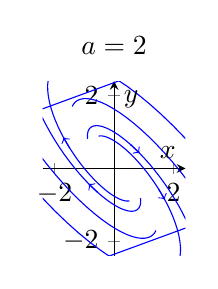
\begin{tikzpicture}\begin{axis}[width=.28\textwidth,height=3.8cm,axis lines=middle,title={$a=2$},xlabel={$x$},ylabel={$y$},xmin=-2.4,xmax=2.4,ymin=-2.4,ymax=2.4,clip=true]\addplot[blue,no marks] coordinates {(-0.51788,0.88895) (-0.46603,0.89495) (-0.40667,0.89360) (-0.33980,0.88439) (-0.26552,0.86691) (-0.18395,0.84073) (-0.09533,0.80550) (0.00006,0.76094) (0.10183,0.70678) (0.20953,0.64287) (0.32263,0.56910) (0.44050,0.48546) (0.56245,0.39200) (0.68768,0.28889) (0.81533,0.17637) (0.94446,0.05478) (1.07404,-0.07543) (1.20298,-0.21370) (1.33012,-0.35937) (1.45424,-0.51169) (1.57405,-0.66976) (1.68824,-0.83261) (1.79542,-0.99914) (1.89421,-1.16815) (1.98318,-1.33835) (2.06091,-1.50834) (2.12597,-1.67663) (2.17694,-1.84164) (2.21245,-2.00173) (2.23113,-2.15517) (2.23172,-2.30019) (2.21299,-2.43498) (2.17381,-2.55766) (2.11315,-2.66638) (2.03009,-2.75925) (1.92387,-2.83440) (1.79385,-2.89000) (1.63956,-2.92426) (1.46071,-2.93544) (1.25722,-2.92191) (1.02920,-2.88213) (0.77698,-2.81468) (0.50114,-2.71830) (0.20247,-2.59189) (-0.11795,-2.43454) (-0.45880,-2.24553) (-0.81849,-2.02438) (-1.19518,-1.77087) (-1.58671,-1.48502) (-1.99071,-1.16715) (-2.40448,-0.81787) (-2.82511,-0.43811) (-3.24940,-0.02912)};\draw[blue,->] (axis cs:1.48897,-0.55630)--(axis cs:1.70338,-0.85525);\addplot[blue,no marks] coordinates {(0.51788,-0.88895) (0.46603,-0.89495) (0.40667,-0.89360) (0.33980,-0.88439) (0.26552,-0.86691) (0.18395,-0.84073) (0.09533,-0.80550) (-0.00006,-0.76094) (-0.10183,-0.70678) (-0.20953,-0.64287) (-0.32263,-0.56910) (-0.44050,-0.48546) (-0.56245,-0.39200) (-0.68768,-0.28889) (-0.81533,-0.17637) (-0.94446,-0.05478) (-1.07404,0.07543) (-1.20298,0.21370) (-1.33012,0.35937) (-1.45424,0.51169) (-1.57405,0.66976) (-1.68824,0.83261) (-1.79542,0.99914) (-1.89421,1.16815) (-1.98318,1.33835) (-2.06091,1.50834) (-2.12597,1.67663) (-2.17694,1.84164) (-2.21245,2.00173) (-2.23113,2.15517) (-2.23172,2.30019) (-2.21299,2.43498) (-2.17381,2.55766) (-2.11315,2.66638) (-2.03009,2.75925) (-1.92387,2.83440) (-1.79385,2.89000) (-1.63956,2.92426) (-1.46071,2.93544) (-1.25722,2.92191) (-1.02920,2.88213) (-0.77698,2.81468) (-0.50114,2.71830) (-0.20247,2.59189) (0.11795,2.43454) (0.45880,2.24553) (0.81849,2.02438) (1.19518,1.77087) (1.58671,1.48502) (1.99071,1.16715) (2.40448,0.81787) (2.82511,0.43811) (3.24940,0.02912)};\draw[blue,->] (axis cs:-1.48897,0.55630)--(axis cs:-1.70338,0.85525);\addplot[blue,no marks] coordinates {(-0.88895,0.81555) (-0.89495,0.87640) (-0.89360,0.93372) (-0.88439,0.98679) (-0.86691,1.03485) (-0.84073,1.07714) (-0.80550,1.11293) (-0.76094,1.14146) (-0.70678,1.16200) (-0.64287,1.17384) (-0.56910,1.17628) (-0.48546,1.16869) (-0.39200,1.15045) (-0.28889,1.12101) (-0.17637,1.07988) (-0.05478,1.02662) (0.07543,0.96090) (0.21370,0.88243) (0.35937,0.79106) (0.51169,0.68671) (0.66976,0.56942) (0.83261,0.43933) (0.99914,0.29672) (1.16815,0.14198) (1.33835,-0.02434) (1.50834,-0.20160) (1.67663,-0.38897) (1.84164,-0.58552) (2.00173,-0.79014) (2.15517,-1.00162) (2.30019,-1.21857) (2.43498,-1.43948) (2.55766,-1.66269) (2.66638,-1.88643) (2.75925,-2.10878) (2.83440,-2.32773) (2.89000,-2.54116) (2.92426,-2.74683) (2.93544,-2.94245) (2.92191,-3.12564) (2.88213,-3.29399) (2.81468,-3.44504) (0.43811,-3.48227) (0.02912,-3.29307) (-0.40751,-3.06264) (-0.86985,-2.79021)};\draw[blue,->] (axis cs:0.55630,0.65452)--(axis cs:0.85525,0.42050);\addplot[blue,no marks] coordinates {(0.88895,-0.81555) (0.89495,-0.87640) (0.89360,-0.93372) (0.88439,-0.98679) (0.86691,-1.03485) (0.84073,-1.07714) (0.80550,-1.11293) (0.76094,-1.14146) (0.70678,-1.16200) (0.64287,-1.17384) (0.56910,-1.17628) (0.48546,-1.16869) (0.39200,-1.15045) (0.28889,-1.12101) (0.17637,-1.07988) (0.05478,-1.02662) (-0.07543,-0.96090) (-0.21370,-0.88243) (-0.35937,-0.79106) (-0.51169,-0.68671) (-0.66976,-0.56942) (-0.83261,-0.43933) (-0.99914,-0.29672) (-1.16815,-0.14198) (-1.33835,0.02434) (-1.50834,0.20160) (-1.67663,0.38897) (-1.84164,0.58552) (-2.00173,0.79014) (-2.15517,1.00162) (-2.30019,1.21857) (-2.43498,1.43948) (-2.55766,1.66269) (-2.66638,1.88643) (-2.75925,2.10878) (-2.83440,2.32773) (-2.89000,2.54116) (-2.92426,2.74683) (-2.93544,2.94245) (-2.92191,3.12564) (-2.88213,3.29399) (-2.81468,3.44504) (-0.43811,3.48227) (-0.02912,3.29307) (0.40751,3.06264) (0.86985,2.79021)};\draw[blue,->] (axis cs:-0.55630,-0.65452)--(axis cs:-0.85525,-0.42050);\addplot[blue,no marks] coordinates {(-1.40683,1.70450) (-1.36098,1.77135) (-1.30026,1.82732) (-1.22420,1.87118) (-1.13242,1.90175) (-1.02468,1.91787) (-0.90083,1.91844) (-0.76087,1.90240) (-0.60495,1.86878) (-0.43333,1.81671) (-0.24647,1.74539) (-0.04495,1.65415) (0.17045,1.54246) (0.39879,1.40990) (0.63897,1.25625) (0.88968,1.08140) (1.14947,0.88547) (1.41668,0.66874) (1.68950,0.43169) (1.96593,0.17503) (2.24381,-0.10034) (2.52084,-0.39328) (2.79456,-0.70242) (3.06236,-1.02617) (3.32154,-1.36270) (-3.22028,-3.32219)};\addplot[blue,no marks] coordinates {(1.40683,-1.70450) (1.36098,-1.77135) (1.30026,-1.82732) (1.22420,-1.87118) (1.13242,-1.90175) (1.02468,-1.91787) (0.90083,-1.91844) (0.76087,-1.90240) (0.60495,-1.86878) (0.43333,-1.81671) (0.24647,-1.74539) (0.04495,-1.65415) (-0.17045,-1.54246) (-0.39879,-1.40990) (-0.63897,-1.25625) (-0.88968,-1.08140) (-1.14947,-0.88547) (-1.41668,-0.66874) (-1.68950,-0.43169) (-1.96593,-0.17503) (-2.24381,0.10034) (-2.52084,0.39328) (-2.79456,0.70242) (-3.06236,1.02617) (-3.32154,1.36270) (3.22028,3.32219)};\end{axis}\end{tikzpicture}\hspace{.035\textwidth}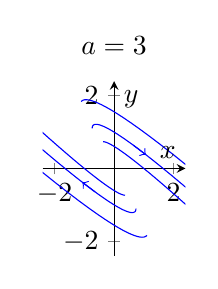
\begin{tikzpicture}\begin{axis}[width=.28\textwidth,height=3.8cm,axis lines=middle,title={$a=3$},xlabel={$x$},ylabel={$y$},xmin=-2.4,xmax=2.4,ymin=-2.4,ymax=2.4,clip=true]\addplot[blue,no marks] coordinates {(-0.36788,0.73576) (-0.34163,0.73415) (-0.31022,0.72902) (-0.27307,0.71991) (-0.22955,0.70631) (-0.17898,0.68767) (-0.12061,0.66336) (-0.05362,0.63271) (0.02288,0.59498) (0.10987,0.54937) (0.20841,0.49497) (0.31965,0.43083) (0.44485,0.35588) (0.58539,0.26896) (0.74276,0.16881) (0.91857,0.05403) (1.11460,-0.07687) (1.33276,-0.22554) (1.57515,-0.39379) (1.84402,-0.58355) (2.14183,-0.79696) (2.47126,-1.03633) (2.83520,-1.30419) (3.23680,-1.60328)};\addplot[blue,no marks] coordinates {(0.36788,-0.73576) (0.34163,-0.73415) (0.31022,-0.72902) (0.27307,-0.71991) (0.22955,-0.70631) (0.17898,-0.68767) (0.12061,-0.66336) (0.05362,-0.63271) (-0.02288,-0.59498) (-0.10987,-0.54937) (-0.20841,-0.49497) (-0.31965,-0.43083) (-0.44485,-0.35588) (-0.58539,-0.26896) (-0.74276,-0.16881) (-0.91857,-0.05403) (-1.11460,0.07687) (-1.33276,0.22554) (-1.57515,0.39379) (-1.84402,0.58355) (-2.14183,0.79696) (-2.47126,1.03633) (-2.83520,1.30419) (-3.23680,1.60328)};\addplot[blue,no marks] coordinates {(-0.73576,1.10364) (-0.73415,1.12666) (-0.72902,1.14781) (-0.71991,1.16675) (-0.70631,1.18307) (-0.68767,1.19635) (-0.66336,1.20611) (-0.63271,1.21180) (-0.59498,1.21285) (-0.54937,1.20861) (-0.49497,1.19836) (-0.43083,1.18132) (-0.35588,1.15662) (-0.26896,1.12332) (-0.16881,1.08037) (-0.05403,1.02664) (0.07687,0.96086) (0.22554,0.88167) (0.39379,0.78757) (0.58355,0.67692) (0.79696,0.54791) (1.03633,0.39859) (1.30419,0.22682) (1.60328,0.03025) (1.93657,-0.19366) (2.30730,-0.44769) (2.71901,-0.73487) (3.17550,-1.05850)};\draw[blue,->] (axis cs:0.64201,0.64201)--(axis cs:1.07132,0.37641);\addplot[blue,no marks] coordinates {(0.73576,-1.10364) (0.73415,-1.12666) (0.72902,-1.14781) (0.71991,-1.16675) (0.70631,-1.18307) (0.68767,-1.19635) (0.66336,-1.20611) (0.63271,-1.21180) (0.59498,-1.21285) (0.54937,-1.20861) (0.49497,-1.19836) (0.43083,-1.18132) (0.35588,-1.15662) (0.26896,-1.12332) (0.16881,-1.08037) (0.05403,-1.02664) (-0.07687,-0.96086) (-0.22554,-0.88167) (-0.39379,-0.78757) (-0.58355,-0.67692) (-0.79696,-0.54791) (-1.03633,-0.39859) (-1.30419,-0.22682) (-1.60328,-0.03025) (-1.93657,0.19366) (-2.30730,0.44769) (-2.71901,0.73487) (-3.17550,1.05850)};\draw[blue,->] (axis cs:-0.64201,-0.64201)--(axis cs:-1.07132,-0.37641);\addplot[blue,no marks] coordinates {(-1.10364,1.83940) (-1.07578,1.86080) (-1.03924,1.87683) (-0.99298,1.88666) (-0.93586,1.88938) (-0.86665,1.88402) (-0.78397,1.86946) (-0.68633,1.84451) (-0.57210,1.80783) (-0.43949,1.75798) (-0.28656,1.69333) (-0.11118,1.61215) (0.08897,1.51250) (0.31643,1.39228) (0.57395,1.24918) (0.86454,1.08067) (1.19147,0.88399) (1.55831,0.65613) (1.96893,0.39379) (2.42756,0.09337) (2.93879,-0.24905)};\addplot[blue,no marks] coordinates {(1.10364,-1.83940) (1.07578,-1.86080) (1.03924,-1.87683) (0.99298,-1.88666) (0.93586,-1.88938) (0.86665,-1.88402) (0.78397,-1.86946) (0.68633,-1.84451) (0.57210,-1.80783) (0.43949,-1.75798) (0.28656,-1.69333) (0.11118,-1.61215) (-0.08897,-1.51250) (-0.31643,-1.39228) (-0.57395,-1.24918) (-0.86454,-1.08067) (-1.19147,-0.88399) (-1.55831,-0.65613) (-1.96893,-0.39379) (-2.42756,-0.09337) (-2.93879,0.24905)};\end{axis}\end{tikzpicture}\par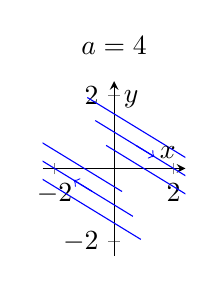
\begin{tikzpicture}\begin{axis}[width=.28\textwidth,height=3.8cm,axis lines=middle,title={$a=4$},xlabel={$x$},ylabel={$y$},xmin=-2.4,xmax=2.4,ymin=-2.4,ymax=2.4,clip=true]\addplot[blue,no marks] coordinates {(-0.26695,0.63348) (-0.25270,0.62635) (-0.23540,0.61770) (-0.21438,0.60719) (-0.18884,0.59442) (-0.15783,0.57891) (-0.12016,0.56008) (-0.07441,0.53720) (-0.01883,0.50942) (0.04867,0.47566) (0.13067,0.43467) (0.23026,0.38487) (0.35122,0.32439) (0.49815,0.25092) (0.67662,0.16169) (0.89339,0.05330) (1.15669,-0.07835) (1.47651,-0.23825) (1.86496,-0.43248) (2.33679,-0.66840) (2.90990,-0.95495)};\addplot[blue,no marks] coordinates {(0.26695,-0.63348) (0.25270,-0.62635) (0.23540,-0.61770) (0.21438,-0.60719) (0.18884,-0.59442) (0.15783,-0.57891) (0.12016,-0.56008) (0.07441,-0.53720) (0.01883,-0.50942) (-0.04867,-0.47566) (-0.13067,-0.43467) (-0.23026,-0.38487) (-0.35122,-0.32439) (-0.49815,-0.25092) (-0.67662,-0.16169) (-0.89339,-0.05330) (-1.15669,0.07835) (-1.47651,0.23825) (-1.86496,0.43248) (-2.33679,0.66840) (-2.90990,0.95495)};\addplot[blue,no marks] coordinates {(-0.63348,1.31674) (-0.62635,1.31318) (-0.61770,1.30885) (-0.60719,1.30359) (-0.59442,1.29721) (-0.57891,1.28946) (-0.56008,1.28004) (-0.53720,1.26860) (-0.50942,1.25471) (-0.47566,1.23783) (-0.43467,1.21733) (-0.38487,1.19244) (-0.32439,1.16219) (-0.25092,1.12546) (-0.16169,1.08084) (-0.05330,1.02665) (0.07835,0.96083) (0.23825,0.88087) (0.43248,0.78376) (0.66840,0.66580) (0.95495,0.52252) (1.30301,0.34850) (1.72577,0.13711) (2.23927,-0.11964) (2.86299,-0.43150)};\draw[blue,->] (axis cs:0.74467,0.62767)--(axis cs:1.35624,0.32188);\addplot[blue,no marks] coordinates {(0.63348,-1.31674) (0.62635,-1.31318) (0.61770,-1.30885) (0.60719,-1.30359) (0.59442,-1.29721) (0.57891,-1.28946) (0.56008,-1.28004) (0.53720,-1.26860) (0.50942,-1.25471) (0.47566,-1.23783) (0.43467,-1.21733) (0.38487,-1.19244) (0.32439,-1.16219) (0.25092,-1.12546) (0.16169,-1.08084) (0.05330,-1.02665) (-0.07835,-0.96083) (-0.23825,-0.88087) (-0.43248,-0.78376) (-0.66840,-0.66580) (-0.95495,-0.52252) (-1.30301,-0.34850) (-1.72577,-0.13711) (-2.23927,0.11964) (-2.86299,0.43150)};\draw[blue,->] (axis cs:-0.74467,-0.62767)--(axis cs:-1.35624,-0.32188);\addplot[blue,no marks] coordinates {(-0.90043,1.95021) (-0.87905,1.93953) (-0.85309,1.92655) (-0.82156,1.91078) (-0.78326,1.89163) (-0.73674,1.86837) (-0.68024,1.84012) (-0.61161,1.80580) (-0.52825,1.76412) (-0.42699,1.71350) (-0.30400,1.65200) (-0.15462,1.57731) (0.02683,1.48658) (0.24723,1.37639) (0.51493,1.24253) (0.84009,1.07996) (1.23504,0.88248) (1.71476,0.64262) (2.29744,0.35128) (3.00519,-0.00260)};\addplot[blue,no marks] coordinates {(0.90043,-1.95021) (0.87905,-1.93953) (0.85309,-1.92655) (0.82156,-1.91078) (0.78326,-1.89163) (0.73674,-1.86837) (0.68024,-1.84012) (0.61161,-1.80580) (0.52825,-1.76412) (0.42699,-1.71350) (0.30400,-1.65200) (0.15462,-1.57731) (-0.02683,-1.48658) (-0.24723,-1.37639) (-0.51493,-1.24253) (-0.84009,-1.07996) (-1.23504,-0.88248) (-1.71476,-0.64262) (-2.29744,-0.35128) (-3.00519,0.00260)};\end{axis}\end{tikzpicture}\hspace{.035\textwidth}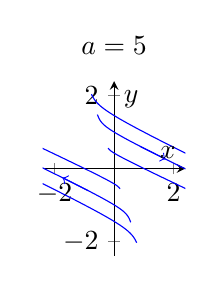
\begin{tikzpicture}\begin{axis}[width=.28\textwidth,height=3.8cm,axis lines=middle,title={$a=5$},xlabel={$x$},ylabel={$y$},xmin=-2.4,xmax=2.4,ymin=-2.4,ymax=2.4,clip=true]\addplot[blue,no marks] coordinates {(-0.19937,0.55982) (-0.19073,0.54918) (-0.18046,0.53802) (-0.16801,0.52614) (-0.15268,0.51327) (-0.13354,0.49905) (-0.10938,0.48302) (-0.07860,0.46456) (-0.03908,0.44287) (0.01195,0.41688) (0.07813,0.38520) (0.16428,0.34599) (0.27672,0.29684) (0.42376,0.23457) (0.61635,0.15498) (0.86890,0.05259) (1.20037,-0.07986) (1.63570,-0.25189) (2.20773,-0.47605) (2.95965,-0.76883)};\addplot[blue,no marks] coordinates {(0.19937,-0.55982) (0.19073,-0.54918) (0.18046,-0.53802) (0.16801,-0.52614) (0.15268,-0.51327) (0.13354,-0.49905) (0.10938,-0.48302) (0.07860,-0.46456) (0.03908,-0.44287) (-0.01195,-0.41688) (-0.07813,-0.38520) (-0.16428,-0.34599) (-0.27672,-0.29684) (-0.42376,-0.23457) (-0.61635,-0.15498) (-0.86890,-0.05259) (-1.20037,0.07986) (-1.63570,0.25189) (-2.20773,0.47605) (-2.95965,0.76883)};\addplot[blue,no marks] coordinates {(-0.55982,1.48009) (-0.54918,1.45680) (-0.53802,1.43360) (-0.52614,1.41042) (-0.51327,1.38714) (-0.49905,1.36362) (-0.48302,1.33969) (-0.46456,1.31510) (-0.44287,1.28954) (-0.41688,1.26260) (-0.38520,1.23374) (-0.34599,1.20227) (-0.29684,1.16724) (-0.23457,1.12745) (-0.15498,1.08130) (-0.05259,1.02667) (0.07986,0.96079) (0.25189,0.88003) (0.47605,0.77959) (0.76883,0.65315) (1.15196,0.49244) (1.65400,0.28651) (2.31258,0.02102) (3.17716,-0.32296)};\draw[blue,->] (axis cs:0.86797,0.61115)--(axis cs:1.73409,0.25400);\addplot[blue,no marks] coordinates {(0.55982,-1.48009) (0.54918,-1.45680) (0.53802,-1.43360) (0.52614,-1.41042) (0.51327,-1.38714) (0.49905,-1.36362) (0.48302,-1.33969) (0.46456,-1.31510) (0.44287,-1.28954) (0.41688,-1.26260) (0.38520,-1.23374) (0.34599,-1.20227) (0.29684,-1.16724) (0.23457,-1.12745) (0.15498,-1.08130) (0.05259,-1.02667) (-0.07986,-0.96079) (-0.25189,-0.88003) (-0.47605,-0.77959) (-0.76883,-0.65315) (-1.15196,-0.49244) (-1.65400,-0.28651) (-2.31258,-0.02102) (-3.17716,0.32296)};\draw[blue,->] (axis cs:-0.86797,-0.61115)--(axis cs:-1.73409,-0.25400);\addplot[blue,no marks] coordinates {(-0.75919,2.03991) (-0.73991,2.00598) (-0.71848,1.97162) (-0.69415,1.93656) (-0.66595,1.90041) (-0.63259,1.86268) (-0.59240,1.82271) (-0.54316,1.77966) (-0.48195,1.73241) (-0.40494,1.67948) (-0.30707,1.61895) (-0.18171,1.54826) (-0.02012,1.46409) (0.18919,1.36202) (0.46137,1.23628) (0.81632,1.07925) (1.28023,0.88093) (1.88760,0.62814) (2.68378,0.30354)};\addplot[blue,no marks] coordinates {(0.75919,-2.03991) (0.73991,-2.00598) (0.71848,-1.97162) (0.69415,-1.93656) (0.66595,-1.90041) (0.63259,-1.86268) (0.59240,-1.82271) (0.54316,-1.77966) (0.48195,-1.73241) (0.40494,-1.67948) (0.30707,-1.61895) (0.18171,-1.54826) (0.02012,-1.46409) (-0.18919,-1.36202) (-0.46137,-1.23628) (-0.81632,-1.07925) (-1.28023,-0.88093) (-1.88760,-0.62814) (-2.68378,-0.30354)};\end{axis}\end{tikzpicture}\end{center}
\par\noindent{\small 依据：官方译审并补证（AI辅助）。}
\end{solution}

\begin{exercise}\label{cw:rec23-4}
给出这八种情形的通解方法，特别处理亏损结点。
\end{exercise}
\begin{solution}
以下公式直接给出每例的所有解，不仅列方法名。令 $h=(a-1)/2,N=A-hI$，Cayley--Hamilton 给 $N^2=d^2I$，$d^2=(a+5)(a-3)/4$。
\[
 u(t)=\begin{cases}
 \ee^{ht}[\cosh(dt)I+\sinh(dt)N/d]c,&d^2>0,\\
 \ee^{ht}[\cos(\beta t)I+\sin(\beta t)N/\beta]c,&d^2=-\beta^2<0,\\
 \ee^{ht}(I+tN)c,&d=0,
 \end{cases}\qquad c\in\mathbb R^2.
\]
对每行求导并用$N^2$即得到$\dot u=Au$；$t=0$矩阵为$I$，故覆盖全部初值。各参数代入为
\[\begin{array}{c|rrrrrrrr}a&-6&-5&-2&1&2&3&4&5\\\hline h&-7/2&-3&-3/2&0&1/2&1&3/2&2\\ d^2&9/4&0&-15/4&-3&-7/4&0&9/4&5\end{array}\]
特别地，$a=-5$时$N=\begin{pmatrix}-2&2\\-2&2\end{pmatrix}$，$a=3$时$N=\begin{pmatrix}2&2\\-2&-2\end{pmatrix}$；两者均$N^2=0,N\ne0$，故$tN$项不可删。这明确补上官方此题未给出的推导。
\par\noindent{\small 依据：官方分类译审；通解与亏损矩阵指数为编者补解（AI辅助）。}
\end{solution}

\originalsection{第24次习题课：矩阵指数与非齐次系统（5月6日）}
本次沿用原题的长期定义：“稳定”指所有解趋于0；“不稳定”指一般初值的解无界；其余称中性稳定。该定义讨论长期极限，不与 Lyapunov 稳定的术语混淆。
\begin{exercise}\label{cw:rec24-1}
在迹--行列式平面，何处能保证所有具有同样$(\tau,\Delta)$的实二阶矩阵稳定、不稳定、中性稳定？有无相同迹与行列式而长期行为不同的矩阵？
\end{exercise}
\begin{solution}
$\tau<0,\Delta>0$ 恰好对应两个根实部负，指数衰减（重根的$t$因子亦被负指数压过），因此稳定。$\Delta<0$有一正一负根，或$\tau>0$有正实部根，均不稳定。
$\tau=0,\Delta>0$时为非零纯虚根，矩阵指数有界周期而不趋于0，中性稳定；$\Delta=0,\tau<0$时根为0与负数，解趋于零特征方向上的常量，亦中性稳定。
剩下原点$(0,0)$：Cayley--Hamilton使$A^2=0$。若$A=0$，全部解常值，中性稳定；若$A\ne0$，$\ee^{At}=I+tA$，一般$c$满足$Ac\ne0$，解线性无界，按本题定义为不稳定。例如$\begin{pmatrix}0&1\\0&0\end{pmatrix}$与零矩阵同迹同列式却不同。以上区域与原点情形覆盖整个平面。
\par\noindent{\small 依据：官方译审并补证（AI辅助）；补幂零边界与本题稳定定义。}
\end{solution}

\begin{exercise}\label{cw:rec24-2}
设$A=\begin{pmatrix}1&1\\-4&1\end{pmatrix}$。
(a) 求基本矩阵$\Phi(t)$；(b) 求$\ee^{At}$；(c) 求初值$u(0)=(1,2)^T$的解；(d) 求$\dot u=Au+(5,10)^T$的一个特解、通解与$u(0)=0$的解。
\end{exercise}
\begin{solution}
(a) $1+2\ii$的特征向量$(1,2\ii)^T$，复解实虚部给
\[\Phi=\ee^t\begin{pmatrix}\cos2t&\sin2t\\-2\sin2t&2\cos2t\end{pmatrix},\quad\det\Phi=2\ee^{2t}\ne0.\]
(b) $\Phi(0)=\diag(1,2)$，因此
\[E(t)=\ee^{At}=\ee^t\begin{pmatrix}\cos2t&\frac12\sin2t\\-2\sin2t&\cos2t\end{pmatrix}.\]
(c) $E(t)(1,2)^T=\ee^t(\cos2t+\sin2t,2\cos2t-2\sin2t)^T$。
(d) 常值特解$p=-A^{-1}(5,10)^T=(1,-6)^T$，直接有$Ap+(5,10)^T=0$。通解$p+E(t)c$；初值零时$c=-p=(-1,6)^T$，故
\[u(t)=\binom{1-\ee^t\cos2t+3\ee^t\sin2t}{-6+2\ee^t\sin2t+6\ee^t\cos2t}.\]
$E(0)=I,E'=AE$检验了全部初值与方程。
\par\noindent{\small 依据：官方译审并补证（AI辅助）。}
\end{solution}

\begin{exercise}\label{cw:rec24-3}
已知常值$u_1=(1,1)^T$和$u_2=(\ee^t,-\ee^t)^T$是$\dot u=Bu$的解。
(a) 求通解，以及初值$(2,2)^T$、$(1,0)^T$的两个解；(b) 求基本矩阵、$\ee^{Bt}$、$\ee^B$；(c) 求$B$的特征值与向量；(d) 求$B$。
\end{exercise}
\begin{solution}
(a) 两初值向量独立，故$u=c_1(1,1)^T+c_2\ee^t(1,-1)^T$。第一初值给常值$(2,2)^T$；第二初值给$u=((1+\ee^t)/2,(1-\ee^t)/2)^T$。
(b) $\Phi=\begin{pmatrix}1&\ee^t\\1&-\ee^t\end{pmatrix}$，$\Phi(0)^{-1}=\frac12\begin{pmatrix}1&1\\1&-1\end{pmatrix}$，故
\[\ee^{Bt}=\frac12\begin{pmatrix}1+\ee^t&1-\ee^t\\1-\ee^t&1+\ee^t\end{pmatrix},\qquad\ee^B=\frac12\begin{pmatrix}1+\ee&1-\ee\\1-\ee&1+\ee\end{pmatrix}.\]
(c) 直接从$Bu_1=u_1'=0$、$Bu_2=u_2'=u_2$得特征值0、1，向量$(1,1)^T,(1,-1)^T$；无需对指数特征值取存在分支歧义的复对数。
(d) 令$P=\begin{pmatrix}1&1\\1&-1\end{pmatrix}$，$B=P\diag(0,1)P^{-1}=\frac12\begin{pmatrix}1&-1\\-1&1\end{pmatrix}$。
\par\noindent{\small 依据：官方译审并补证（AI辅助）。}
\end{solution}

\originalsection{第25次习题课：自治系统与生态模型（5月11日）}
令$x$为昆虫种群、$y$为鸟类种群，使用题设的方便单位。模型 $\dot x=(2-x-y)x,\dot y=(x-1)y$ 表示鸟捕食虫：无鸟时虫 logistic 增长，无虫时鸟指数消亡。
\begin{exercise}\label{cw:rec25-1}
求系统所有临界点（平衡点）。
\end{exercise}
\begin{solution}
同时解$x(2-x-y)=0,y(x-1)=0$。若$x=0$则$y=0$；若$y=0$且$x\ne0$则$x=2$；若两者非零则$x=1,y=1$。所以全部为$(0,0),(2,0),(1,1)$，没有遗漏其他实平衡。
\par\noindent{\small 依据：官方译审并补证（AI辅助）。}
\end{solution}

\begin{exercise}\label{cw:rec25-2}
在每个平衡点求线性化，画附近轨迹。
\end{exercise}
\begin{solution}
Jacobian为$J=\begin{pmatrix}2-2x-y&-x\\y&x-1\end{pmatrix}$。
在$(0,0)$为$\diag(2,-1)$：鞍点，$x$轴向外、$y$轴向内。
在$(2,0)$为$\begin{pmatrix}-2&-2\\0&1\end{pmatrix}$：鞍点，稳定方向$(1,0)$，不稳定方向$(2,-3)$（斜率$-3/2$）。
在$(1,1)$为$\begin{pmatrix}-1&-1\\1&0\end{pmatrix}$：特征值$(-1\pm\ii\sqrt3)/2$，逆时针稳定螺旋。三个均双曲，线性化决定局部相图类型；图中坐标为相对平衡点的扰动$(\xi,\eta)$（小图的$x,y$轴分别指这两个扰动）。\begin{center}\begin{tikzpicture}\begin{axis}[width=.28\textwidth,height=3.8cm,axis lines=middle,title={原点附近},xlabel={$x$},ylabel={$y$},xmin=-2.4,xmax=2.4,ymin=-2.4,ymax=2.4,clip=true]\addplot[blue,no marks] coordinates {(0.13534,0.00000) (0.15695,0.00000) (0.18201,0.00000) (0.21107,0.00000) (0.24478,0.00000) (0.28386,0.00000) (0.32919,0.00000) (0.38176,0.00000) (0.44272,0.00000) (0.51342,0.00000) (0.59540,0.00000) (0.69048,0.00000) (0.80074,0.00000) (0.92860,0.00000) (1.07689,0.00000) (1.24885,0.00000) (1.44827,0.00000) (1.67954,0.00000) (1.94773,0.00000) (2.25876,0.00000) (2.61945,0.00000) (3.03773,0.00000)};\draw[blue,->] (axis cs:1.64872,0.00000)--(axis cs:2.09594,0.00000);\addplot[blue,no marks] coordinates {(-0.13534,0.00000) (-0.15695,0.00000) (-0.18201,0.00000) (-0.21107,0.00000) (-0.24478,0.00000) (-0.28386,0.00000) (-0.32919,0.00000) (-0.38176,0.00000) (-0.44272,0.00000) (-0.51342,0.00000) (-0.59540,0.00000) (-0.69048,0.00000) (-0.80074,0.00000) (-0.92860,0.00000) (-1.07689,0.00000) (-1.24885,0.00000) (-1.44827,0.00000) (-1.67954,0.00000) (-1.94773,0.00000) (-2.25876,0.00000) (-2.61945,0.00000) (-3.03773,0.00000)};\draw[blue,->] (axis cs:-1.64872,0.00000)--(axis cs:-2.09594,0.00000);\addplot[blue,no marks] coordinates {(0.00000,2.71828) (0.00000,2.52420) (0.00000,2.34398) (0.00000,2.17663) (0.00000,2.02122) (0.00000,1.87692) (0.00000,1.74291) (0.00000,1.61847) (0.00000,1.50292) (0.00000,1.39561) (0.00000,1.29597) (0.00000,1.20344) (0.00000,1.11752) (0.00000,1.03773) (0.00000,0.96364) (0.00000,0.89484) (0.00000,0.83095) (0.00000,0.77162) (0.00000,0.71653) (0.00000,0.66537) (0.00000,0.61787) (0.00000,0.57375) (0.00000,0.53279) (0.00000,0.49475) (0.00000,0.45943) (0.00000,0.42662) (0.00000,0.39616) (0.00000,0.36788) (0.00000,0.34161) (0.00000,0.31722) (0.00000,0.29457) (0.00000,0.27354) (0.00000,0.25401) (0.00000,0.23588) (0.00000,0.21904) (0.00000,0.20340) (0.00000,0.18888) (0.00000,0.17539) (0.00000,0.16287) (0.00000,0.15124) (0.00000,0.14044) (0.00000,0.13041) (0.00000,0.12110) (0.00000,0.11246) (0.00000,0.10443) (0.00000,0.09697) (0.00000,0.09005) (0.00000,0.08362) (0.00000,0.07765) (0.00000,0.07211) (0.00000,0.06696) (0.00000,0.06218) (0.00000,0.05774) (0.00000,0.05362) (0.00000,0.04979)};\draw[blue,->] (axis cs:0.00000,0.77880)--(axis cs:0.00000,0.69073);\addplot[blue,no marks] coordinates {(0.00000,-2.71828) (0.00000,-2.52420) (0.00000,-2.34398) (0.00000,-2.17663) (0.00000,-2.02122) (0.00000,-1.87692) (0.00000,-1.74291) (0.00000,-1.61847) (0.00000,-1.50292) (0.00000,-1.39561) (0.00000,-1.29597) (0.00000,-1.20344) (0.00000,-1.11752) (0.00000,-1.03773) (0.00000,-0.96364) (0.00000,-0.89484) (0.00000,-0.83095) (0.00000,-0.77162) (0.00000,-0.71653) (0.00000,-0.66537) (0.00000,-0.61787) (0.00000,-0.57375) (0.00000,-0.53279) (0.00000,-0.49475) (0.00000,-0.45943) (0.00000,-0.42662) (0.00000,-0.39616) (0.00000,-0.36788) (0.00000,-0.34161) (0.00000,-0.31722) (0.00000,-0.29457) (0.00000,-0.27354) (0.00000,-0.25401) (0.00000,-0.23588) (0.00000,-0.21904) (0.00000,-0.20340) (0.00000,-0.18888) (0.00000,-0.17539) (0.00000,-0.16287) (0.00000,-0.15124) (0.00000,-0.14044) (0.00000,-0.13041) (0.00000,-0.12110) (0.00000,-0.11246) (0.00000,-0.10443) (0.00000,-0.09697) (0.00000,-0.09005) (0.00000,-0.08362) (0.00000,-0.07765) (0.00000,-0.07211) (0.00000,-0.06696) (0.00000,-0.06218) (0.00000,-0.05774) (0.00000,-0.05362) (0.00000,-0.04979)};\draw[blue,->] (axis cs:0.00000,-0.77880)--(axis cs:0.00000,-0.69073);\addplot[blue,no marks] coordinates {(0.13534,2.71828) (0.15695,2.52420) (0.18201,2.34398) (0.21107,2.17663) (0.24478,2.02122) (0.28386,1.87692) (0.32919,1.74291) (0.38176,1.61847) (0.44272,1.50292) (0.51342,1.39561) (0.59540,1.29597) (0.69048,1.20344) (0.80074,1.11752) (0.92860,1.03773) (1.07689,0.96364) (1.24885,0.89484) (1.44827,0.83095) (1.67954,0.77162) (1.94773,0.71653) (2.25876,0.66537) (2.61945,0.61787) (3.03773,0.57375)};\draw[blue,->] (axis cs:1.64872,0.77880)--(axis cs:2.09594,0.69073);\addplot[blue,no marks] coordinates {(-0.13534,-2.71828) (-0.15695,-2.52420) (-0.18201,-2.34398) (-0.21107,-2.17663) (-0.24478,-2.02122) (-0.28386,-1.87692) (-0.32919,-1.74291) (-0.38176,-1.61847) (-0.44272,-1.50292) (-0.51342,-1.39561) (-0.59540,-1.29597) (-0.69048,-1.20344) (-0.80074,-1.11752) (-0.92860,-1.03773) (-1.07689,-0.96364) (-1.24885,-0.89484) (-1.44827,-0.83095) (-1.67954,-0.77162) (-1.94773,-0.71653) (-2.25876,-0.66537) (-2.61945,-0.61787) (-3.03773,-0.57375)};\draw[blue,->] (axis cs:-1.64872,-0.77880)--(axis cs:-2.09594,-0.69073);\end{axis}\end{tikzpicture}\hspace{.035\textwidth}\begin{tikzpicture}\begin{axis}[width=.28\textwidth,height=3.8cm,axis lines=middle,title={$(2,0)$附近},xlabel={$x$},ylabel={$y$},xmin=-2.4,xmax=2.4,ymin=-2.4,ymax=2.4,clip=true]\addplot[blue,no marks] coordinates {(3.03773,0.00000) (2.61945,0.00000) (2.25876,0.00000) (1.94773,0.00000) (1.67954,0.00000) (1.44827,0.00000) (1.24885,0.00000) (1.07689,0.00000) (0.92860,0.00000) (0.80074,0.00000) (0.69048,0.00000) (0.59540,0.00000) (0.51342,0.00000) (0.44272,0.00000) (0.38176,0.00000) (0.32919,0.00000) (0.28386,0.00000) (0.24478,0.00000) (0.21107,0.00000) (0.18201,0.00000) (0.15695,0.00000) (0.13534,0.00000) (0.11670,0.00000) (0.10063,0.00000) (0.08677,0.00000) (0.07483,0.00000) (0.06452,0.00000) (0.05564,0.00000) (0.04798,0.00000) (0.04137,0.00000) (0.03567,0.00000) (0.03076,0.00000) (0.02653,0.00000) (0.02287,0.00000) (0.01972,0.00000) (0.01701,0.00000) (0.01467,0.00000) (0.01265,0.00000) (0.01091,0.00000) (0.00940,0.00000) (0.00811,0.00000) (0.00699,0.00000) (0.00603,0.00000) (0.00520,0.00000) (0.00448,0.00000) (0.00387,0.00000) (0.00333,0.00000) (0.00287,0.00000) (0.00248,0.00000)};\draw[blue,->] (axis cs:0.60653,0.00000)--(axis cs:0.47711,0.00000);\addplot[blue,no marks] coordinates {(-3.03773,0.00000) (-2.61945,0.00000) (-2.25876,0.00000) (-1.94773,0.00000) (-1.67954,0.00000) (-1.44827,0.00000) (-1.24885,0.00000) (-1.07689,0.00000) (-0.92860,0.00000) (-0.80074,0.00000) (-0.69048,0.00000) (-0.59540,0.00000) (-0.51342,0.00000) (-0.44272,0.00000) (-0.38176,0.00000) (-0.32919,0.00000) (-0.28386,0.00000) (-0.24478,0.00000) (-0.21107,0.00000) (-0.18201,0.00000) (-0.15695,0.00000) (-0.13534,0.00000) (-0.11670,0.00000) (-0.10063,0.00000) (-0.08677,0.00000) (-0.07483,0.00000) (-0.06452,0.00000) (-0.05564,0.00000) (-0.04798,0.00000) (-0.04137,0.00000) (-0.03567,0.00000) (-0.03076,0.00000) (-0.02653,0.00000) (-0.02287,0.00000) (-0.01972,0.00000) (-0.01701,0.00000) (-0.01467,0.00000) (-0.01265,0.00000) (-0.01091,0.00000) (-0.00940,0.00000) (-0.00811,0.00000) (-0.00699,0.00000) (-0.00603,0.00000) (-0.00520,0.00000) (-0.00448,0.00000) (-0.00387,0.00000) (-0.00333,0.00000) (-0.00287,0.00000) (-0.00248,0.00000)};\draw[blue,->] (axis cs:-0.60653,0.00000)--(axis cs:-0.47711,0.00000);\addplot[blue,no marks] coordinates {(3.37842,0.42662) (2.85219,0.45943) (2.39373,0.49475) (1.99335,0.53279) (1.64265,0.57375) (1.33439,0.61787) (1.06226,0.66537) (0.82080,0.71653) (0.60528,0.77162) (0.41155,0.83095) (0.23601,0.89484) (0.07550,0.96364) (-0.07275,1.03773) (-0.21119,1.11752) (-0.34198,1.20344) (-0.46705,1.29597) (-0.58813,1.39561) (-0.70680,1.50292) (-0.82447,1.61847) (-0.94248,1.74291) (-1.06203,1.87692) (-1.18430,2.02122) (-1.31037,2.17663) (-1.44132,2.34398) (-1.57817,2.52420) (-1.72196,2.71828) (-1.87372,2.92728) (-2.03448,3.15235) (-2.20530,3.39472)};\draw[blue,->] (axis cs:-0.45166,1.28403)--(axis cs:-0.64708,1.44773);\addplot[blue,no marks] coordinates {(-3.37842,-0.42662) (-2.85219,-0.45943) (-2.39373,-0.49475) (-1.99335,-0.53279) (-1.64265,-0.57375) (-1.33439,-0.61787) (-1.06226,-0.66537) (-0.82080,-0.71653) (-0.60528,-0.77162) (-0.41155,-0.83095) (-0.23601,-0.89484) (-0.07550,-0.96364) (0.07275,-1.03773) (0.21119,-1.11752) (0.34198,-1.20344) (0.46705,-1.29597) (0.58813,-1.39561) (0.70680,-1.50292) (0.82447,-1.61847) (0.94248,-1.74291) (1.06203,-1.87692) (1.18430,-2.02122) (1.31037,-2.17663) (1.44132,-2.34398) (1.57817,-2.52420) (1.72196,-2.71828) (1.87372,-2.92728) (2.03448,-3.15235) (2.20530,-3.39472)};\draw[blue,->] (axis cs:0.45166,-1.28403)--(axis cs:0.64708,-1.44773);\addplot[blue,no marks] coordinates {(3.32101,0.66537) (2.76854,0.71653) (2.28481,0.77162) (1.85982,0.83095) (1.48486,0.89484) (1.15238,0.96364) (0.85585,1.03773) (0.58955,1.11752) (0.34850,1.20344) (0.12836,1.29597) (-0.07471,1.39561) (-0.26408,1.50292) (-0.44271,1.61847) (-0.61328,1.74291) (-0.77817,1.87692) (-0.93952,2.02122) (-1.09930,2.17663) (-1.25931,2.34398) (-1.42123,2.52420) (-1.58663,2.71828) (-1.75702,2.92728) (-1.93385,3.15235) (-2.11852,3.39472)};\draw[blue,->] (axis cs:0.15487,1.28403)--(axis cs:-0.16997,1.44773);\addplot[blue,no marks] coordinates {(-3.32101,-0.66537) (-2.76854,-0.71653) (-2.28481,-0.77162) (-1.85982,-0.83095) (-1.48486,-0.89484) (-1.15238,-0.96364) (-0.85585,-1.03773) (-0.58955,-1.11752) (-0.34850,-1.20344) (-0.12836,-1.29597) (0.07471,-1.39561) (0.26408,-1.50292) (0.44271,-1.61847) (0.61328,-1.74291) (0.77817,-1.87692) (0.93952,-2.02122) (1.09930,-2.17663) (1.25931,-2.34398) (1.42123,-2.52420) (1.58663,-2.71828) (1.75702,-2.92728) (1.93385,-3.15235) (2.11852,-3.39472)};\draw[blue,->] (axis cs:-0.15487,-1.28403)--(axis cs:0.16997,-1.44773);\end{axis}\end{tikzpicture}\hspace{.035\textwidth}\begin{tikzpicture}\begin{axis}[width=.28\textwidth,height=3.8cm,axis lines=middle,title={$(1,1)$附近},xlabel={$x$},ylabel={$y$},xmin=-2.4,xmax=2.4,ymin=-2.4,ymax=2.4,clip=true]\addplot[blue,no marks] coordinates {(1.79325,-1.45022) (1.73725,-1.22115) (1.66071,-1.00071) (1.56734,-0.79132) (1.46066,-0.59494) (1.34396,-0.41307) (1.22029,-0.24681) (1.09246,-0.09688) (0.96297,0.03635) (0.83407,0.15281) (0.70772,0.25270) (0.58559,0.33647) (0.46909,0.40477) (0.35937,0.45838) (0.25734,0.49827) (0.16366,0.52546) (0.07880,0.54108) (0.00301,0.54628) (-0.06361,0.54226) (-0.12113,0.53019) (-0.16975,0.51124) (-0.20979,0.48655) (-0.24165,0.45720) (-0.26584,0.42423) (-0.28291,0.38859) (-0.29345,0.35116) (-0.29809,0.31276) (-0.29747,0.27411) (-0.29225,0.23584) (-0.28306,0.19851) (-0.27053,0.16260) (-0.25527,0.12849) (-0.23785,0.09651) (-0.21880,0.06690) (-0.19863,0.03983) (-0.17778,0.01543) (-0.15667,-0.00624) (-0.13566,-0.02519) (-0.11506,-0.04143) (-0.09517,-0.05505) (-0.07619,-0.06615) (-0.05832,-0.07485) (-0.04171,-0.08132) (-0.02645,-0.08572) (-0.01264,-0.08824) (-0.00031,-0.08906) (0.01053,-0.08839) (0.01988,-0.08640) (0.02779,-0.08329) (0.03429,-0.07925) (0.03947,-0.07446) (0.04339,-0.06908) (0.04616,-0.06326) (0.04786,-0.05715) (0.04860,-0.05089)};\draw[blue,->] (axis cs:0.75244,0.21890)--(axis cs:0.63766,0.30227);\addplot[blue,no marks] coordinates {(-1.79325,1.45022) (-1.73725,1.22115) (-1.66071,1.00071) (-1.56734,0.79132) (-1.46066,0.59494) (-1.34396,0.41307) (-1.22029,0.24681) (-1.09246,0.09688) (-0.96297,-0.03635) (-0.83407,-0.15281) (-0.70772,-0.25270) (-0.58559,-0.33647) (-0.46909,-0.40477) (-0.35937,-0.45838) (-0.25734,-0.49827) (-0.16366,-0.52546) (-0.07880,-0.54108) (-0.00301,-0.54628) (0.06361,-0.54226) (0.12113,-0.53019) (0.16975,-0.51124) (0.20979,-0.48655) (0.24165,-0.45720) (0.26584,-0.42423) (0.28291,-0.38859) (0.29345,-0.35116) (0.29809,-0.31276) (0.29747,-0.27411) (0.29225,-0.23584) (0.28306,-0.19851) (0.27053,-0.16260) (0.25527,-0.12849) (0.23785,-0.09651) (0.21880,-0.06690) (0.19863,-0.03983) (0.17778,-0.01543) (0.15667,0.00624) (0.13566,0.02519) (0.11506,0.04143) (0.09517,0.05505) (0.07619,0.06615) (0.05832,0.07485) (0.04171,0.08132) (0.02645,0.08572) (0.01264,0.08824) (0.00031,0.08906) (-0.01053,0.08839) (-0.01988,0.08640) (-0.02779,0.08329) (-0.03429,0.07925) (-0.03947,0.07446) (-0.04339,0.06908) (-0.04616,0.06326) (-0.04786,0.05715) (-0.04860,0.05089)};\draw[blue,->] (axis cs:-0.75244,-0.21890)--(axis cs:-0.63766,-0.30227);\addplot[blue,no marks] coordinates {(1.45022,0.34303) (1.22115,0.51609) (1.00071,0.66000) (0.79132,0.77602) (0.59494,0.86572) (0.41307,0.93089) (0.24681,0.97348) (0.09688,0.99558) (-0.03635,0.99932) (-0.15281,0.98688) (-0.25270,0.96042) (-0.33647,0.92206) (-0.40477,0.87386) (-0.45838,0.81776) (-0.49827,0.75561) (-0.52546,0.68913) (-0.54108,0.61988) (-0.54628,0.54930) (-0.54226,0.47865) (-0.53019,0.40906) (-0.51124,0.34149) (-0.48655,0.27676) (-0.45720,0.21555) (-0.42423,0.15838) (-0.38859,0.10568) (-0.35116,0.05772) (-0.31276,0.01468) (-0.27411,-0.02336) (-0.23584,-0.05640) (-0.19851,-0.08454) (-0.16260,-0.10793) (-0.12849,-0.12678) (-0.09651,-0.14134) (-0.06690,-0.15190) (-0.03983,-0.15879) (-0.01543,-0.16234) (0.00624,-0.16291) (0.02519,-0.16084) (0.04143,-0.15650) (0.05505,-0.15022) (0.06615,-0.14233) (0.07485,-0.13317) (0.08132,-0.12302) (0.08572,-0.11218) (0.08824,-0.10088) (0.08906,-0.08937) (0.08839,-0.07786) (0.08640,-0.06651) (0.08329,-0.05551) (0.07925,-0.04496) (0.07446,-0.03499) (0.06908,-0.02568) (0.06326,-0.01710) (0.05715,-0.00929) (0.05089,-0.00229)};\draw[blue,->] (axis cs:-0.21890,0.97135)--(axis cs:-0.30227,0.93994);\addplot[blue,no marks] coordinates {(-1.45022,-0.34303) (-1.22115,-0.51609) (-1.00071,-0.66000) (-0.79132,-0.77602) (-0.59494,-0.86572) (-0.41307,-0.93089) (-0.24681,-0.97348) (-0.09688,-0.99558) (0.03635,-0.99932) (0.15281,-0.98688) (0.25270,-0.96042) (0.33647,-0.92206) (0.40477,-0.87386) (0.45838,-0.81776) (0.49827,-0.75561) (0.52546,-0.68913) (0.54108,-0.61988) (0.54628,-0.54930) (0.54226,-0.47865) (0.53019,-0.40906) (0.51124,-0.34149) (0.48655,-0.27676) (0.45720,-0.21555) (0.42423,-0.15838) (0.38859,-0.10568) (0.35116,-0.05772) (0.31276,-0.01468) (0.27411,0.02336) (0.23584,0.05640) (0.19851,0.08454) (0.16260,0.10793) (0.12849,0.12678) (0.09651,0.14134) (0.06690,0.15190) (0.03983,0.15879) (0.01543,0.16234) (-0.00624,0.16291) (-0.02519,0.16084) (-0.04143,0.15650) (-0.05505,0.15022) (-0.06615,0.14233) (-0.07485,0.13317) (-0.08132,0.12302) (-0.08572,0.11218) (-0.08824,0.10088) (-0.08906,0.08937) (-0.08839,0.07786) (-0.08640,0.06651) (-0.08329,0.05551) (-0.07925,0.04496) (-0.07446,0.03499) (-0.06908,0.02568) (-0.06326,0.01710) (-0.05715,0.00929) (-0.05089,0.00229)};\draw[blue,->] (axis cs:0.21890,-0.97135)--(axis cs:0.30227,-0.93994);\addplot[blue,no marks] coordinates {(3.24347,-1.10719) (2.95840,-0.70506) (2.66142,-0.34072) (2.35867,-0.01531) (2.05560,0.27078) (1.75702,0.51782) (1.46710,0.72668) (1.18933,0.89870) (0.92662,1.03567) (0.68126,1.13969) (0.45502,1.21312) (0.24911,1.25854) (0.06433,1.27862) (-0.09901,1.27614) (-0.24093,1.25388) (-0.36180,1.21459) (-0.46228,1.16096) (-0.54327,1.09558) (-0.60587,1.02091) (-0.65132,0.93924) (-0.68099,0.85273) (-0.69634,0.76331) (-0.69886,0.67275) (-0.69007,0.58261) (-0.67150,0.49427) (-0.64461,0.40888) (-0.61085,0.32744) (-0.57158,0.25075) (-0.52809,0.17944) (-0.48157,0.11397) (-0.43313,0.05467) (-0.38377,0.00172) (-0.33436,-0.04483) (-0.28570,-0.08500) (-0.23846,-0.11896) (-0.19321,-0.14691) (-0.15042,-0.16916) (-0.11047,-0.18603) (-0.07363,-0.19793) (-0.04012,-0.20527) (-0.01004,-0.20848) (0.01653,-0.20802) (0.03961,-0.20434) (0.05927,-0.19790) (0.07560,-0.18912) (0.08875,-0.17844) (0.09891,-0.16624) (0.10628,-0.15291) (0.11108,-0.13880) (0.11355,-0.12421) (0.11393,-0.10945) (0.11247,-0.09476) (0.10942,-0.08036) (0.10502,-0.06645) (0.09950,-0.05318)};\draw[blue,->] (axis cs:0.53354,1.19025)--(axis cs:0.33539,1.24221);\addplot[blue,no marks] coordinates {(-3.24347,1.10719) (-2.95840,0.70506) (-2.66142,0.34072) (-2.35867,0.01531) (-2.05560,-0.27078) (-1.75702,-0.51782) (-1.46710,-0.72668) (-1.18933,-0.89870) (-0.92662,-1.03567) (-0.68126,-1.13969) (-0.45502,-1.21312) (-0.24911,-1.25854) (-0.06433,-1.27862) (0.09901,-1.27614) (0.24093,-1.25388) (0.36180,-1.21459) (0.46228,-1.16096) (0.54327,-1.09558) (0.60587,-1.02091) (0.65132,-0.93924) (0.68099,-0.85273) (0.69634,-0.76331) (0.69886,-0.67275) (0.69007,-0.58261) (0.67150,-0.49427) (0.64461,-0.40888) (0.61085,-0.32744) (0.57158,-0.25075) (0.52809,-0.17944) (0.48157,-0.11397) (0.43313,-0.05467) (0.38377,-0.00172) (0.33436,0.04483) (0.28570,0.08500) (0.23846,0.11896) (0.19321,0.14691) (0.15042,0.16916) (0.11047,0.18603) (0.07363,0.19793) (0.04012,0.20527) (0.01004,0.20848) (-0.01653,0.20802) (-0.03961,0.20434) (-0.05927,0.19790) (-0.07560,0.18912) (-0.08875,0.17844) (-0.09891,0.16624) (-0.10628,0.15291) (-0.11108,0.13880) (-0.11355,0.12421) (-0.11393,0.10945) (-0.11247,0.09476) (-0.10942,0.08036) (-0.10502,0.06645) (-0.09950,0.05318)};\draw[blue,->] (axis cs:-0.53354,-1.19025)--(axis cs:-0.33539,-1.24221);\end{axis}\end{tikzpicture}\end{center}
\par\noindent{\small 依据：官方译审并补证（AI辅助）。}
\end{solution}

\begin{exercise}\label{cw:rec25-3}
在虫--鸟平面标出仅有昆虫和仅有鸟时的相线；结合线性化画完整种群相图。
\end{exercise}
\begin{solution}
坐标轴不变：$y=0$时$\dot x=x(2-x)$，$0<x<2$向右，$x>2$向左；$x=0$时$\dot y=-y$，向原点。第一象限内，$x+y<2$时$x$增加，$x+y>2$时减少；$x>1$时$y$增加，$x<1$时减少。
不仅局部可以判断，所有正初值都趋于$(1,1)$。取
\[V=x-1-\log x+y-1-\log y\ge0,\qquad\dot V=-(x-1)^2\le0.\]
正初值的子水平集在第一象限内紧致，远离坐标轴，所以解全局存在并有非空紧的极限集。该极限集必须位于$\dot V=0$的$x=1$上：否则负导数邻域的反复进入会使$V$下降超过其有限下界。极限集又随流不变，而$x=1$上$\dot x=1-y$，仅$y=1$能留在线上。因此唯一极限点为$(1,1)$。图中蓝线为方程数值积分所得示意轨迹，虚线为$x=1$及$x+y=2$；收敛由上述论证支持。
\begin{center}\begin{tikzpicture}\begin{axis}[width=.65\textwidth,height=5cm,axis lines=middle,xlabel={昆虫$x$},ylabel={鸟类$y$},xmin=0,xmax=2.7,ymin=0,ymax=2.8,clip=true]\addplot[blue]coordinates{(0.80000,0.40000)(0.86462,0.39330)(0.92892,0.38924)(0.99188,0.38769)(1.05257,0.38857)(1.11010,0.39178)(1.16373,0.39723)(1.21285,0.40485)(1.25701,0.41456)(1.29594,0.42629)(1.32950,0.43995)(1.35771,0.45546)(1.38066,0.47274)(1.39856,0.49168)(1.41168,0.51218)(1.42032,0.53411)(1.42483,0.55735)(1.42555,0.58176)(1.42285,0.60717)(1.41707,0.63342)(1.40855,0.66032)(1.39763,0.68769)(1.38463,0.71534)(1.36985,0.74305)(1.35357,0.77063)(1.33607,0.79787)(1.31761,0.82458)(1.29841,0.85056)(1.27871,0.87565)(1.25872,0.89967)(1.23861,0.92249)(1.21857,0.94398)(1.19876,0.96402)(1.17931,0.98255)(1.16035,0.99950)(1.14198,1.01483)(1.12430,1.02852)(1.10739,1.04058)(1.09131,1.05104)(1.07611,1.05993)(1.06183,1.06731)(1.04850,1.07325)(1.03612,1.07783)(1.02472,1.08113)(1.01427,1.08324)(1.00479,1.08427)(0.99624,1.08432)(0.98861,1.08349)(0.98187,1.08187)(0.97599,1.07957)(0.97094,1.07668)(0.96667,1.07329)(0.96314,1.06950)(0.96032,1.06538)(0.95816,1.06101)(0.95661,1.05646)(0.95562,1.05180)(0.95516,1.04708)(0.95518,1.04235)(0.95562,1.03768)(0.95645,1.03309)(0.95762,1.02863)(0.95909,1.02432)(0.96081,1.02019)(0.96275,1.01627)(0.96487,1.01257)(0.96712,1.00911)(0.96949,1.00589)(0.97192,1.00293)(0.97440,1.00022)(0.97689,0.99777)(0.97938,0.99558)(0.98183,0.99364)(0.98422,0.99194)(0.98655,0.99048)(0.98878,0.98925)(0.99092,0.98824)(0.99294,0.98744)(0.99484,0.98683)(0.99661,0.98641)(0.99825,0.98616)(0.99975,0.98606)(1.00111,0.98610)(1.00233,0.98627)(1.00341,0.98656)(1.00436,0.98695)(1.00517,0.98742)(1.00586,0.98797)(1.00642,0.98858)(1.00687,0.98924)(1.00721,0.98995)(1.00745,0.99068)(1.00759,0.99143)(1.00765,0.99219)(1.00763,0.99296)(1.00753,0.99372)(1.00738,0.99446)(1.00716,0.99519)(1.00690,0.99590)(1.00660,0.99658)(1.00626,0.99722)(1.00589,0.99783)(1.00551,0.99841)(1.00510,0.99894)(1.00469,0.99943)(1.00427,0.99988)(1.00385,1.00029)(1.00343,1.00066)(1.00302,1.00099)(1.00263,1.00127)(1.00224,1.00152)(1.00187,1.00172)(1.00151,1.00189)(1.00118,1.00203)(1.00087,1.00213)(1.00058,1.00220)(1.00031,1.00225)(1.00006,1.00227)(0.99984,1.00226)(0.99964,1.00224)(0.99946,1.00219)(0.99931,1.00213)(0.99917,1.00205)(0.99906,1.00196)(0.99897,1.00186)(0.99889,1.00175)(0.99884,1.00164)(0.99880,1.00152)(0.99877,1.00140)(0.99876,1.00127)(0.99877,1.00115)(0.99878,1.00102)(0.99880,1.00090)(0.99884,1.00078)(0.99888,1.00067)(0.99893,1.00056)(0.99898,1.00045)(0.99904,1.00035)(0.99910,1.00026)(0.99917,1.00017)};\draw[blue,->](axis cs:0.99055,0.38770)--(axis cs:1.10811,0.39162);\addplot[blue]coordinates{(2.00000,0.80000)(1.85199,0.87802)(1.72557,0.95047)(1.61565,1.01676)(1.51885,1.07644)(1.43289,1.12919)(1.35616,1.17488)(1.28748,1.21351)(1.22596,1.24523)(1.17091,1.27030)(1.12172,1.28910)(1.07792,1.30207)(1.03908,1.30971)(1.00480,1.31256)(0.97473,1.31116)(0.94856,1.30606)(0.92598,1.29780)(0.90673,1.28688)(0.89054,1.27378)(0.87718,1.25893)(0.86642,1.24276)(0.85806,1.22561)(0.85189,1.20781)(0.84775,1.18966)(0.84545,1.17141)(0.84483,1.15326)(0.84572,1.13541)(0.84799,1.11802)(0.85148,1.10122)(0.85606,1.08511)(0.86158,1.06978)(0.86793,1.05530)(0.87496,1.04172)(0.88257,1.02907)(0.89063,1.01738)(0.89904,1.00666)(0.90768,0.99691)(0.91645,0.98812)(0.92526,0.98027)(0.93403,0.97335)(0.94266,0.96733)(0.95110,0.96217)(0.95926,0.95784)(0.96710,0.95429)(0.97456,0.95150)(0.98160,0.94940)(0.98819,0.94796)(0.99430,0.94713)(0.99992,0.94686)(1.00502,0.94710)(1.00961,0.94780)(1.01368,0.94892)(1.01725,0.95040)(1.02032,0.95221)(1.02290,0.95428)(1.02502,0.95659)(1.02671,0.95909)(1.02797,0.96174)(1.02885,0.96450)(1.02936,0.96733)(1.02954,0.97021)(1.02942,0.97310)(1.02903,0.97597)(1.02840,0.97880)(1.02755,0.98156)(1.02652,0.98424)(1.02533,0.98681)(1.02402,0.98927)(1.02260,0.99159)(1.02110,0.99378)(1.01955,0.99582)(1.01795,0.99770)(1.01634,0.99942)(1.01473,1.00099)(1.01314,1.00239)(1.01157,1.00364)(1.01004,1.00473)(1.00856,1.00568)(1.00715,1.00647)(1.00580,1.00713)(1.00453,1.00765)(1.00334,1.00805)(1.00223,1.00833)(1.00121,1.00851)(1.00027,1.00858)(0.99942,1.00856)(0.99866,1.00847)(0.99799,1.00830)(0.99740,1.00806)(0.99689,1.00777)(0.99646,1.00743)(0.99611,1.00705)(0.99583,1.00665)(0.99561,1.00621)(0.99546,1.00576)(0.99537,1.00529)(0.99533,1.00482)(0.99533,1.00435)(0.99539,1.00388)(0.99548,1.00342)(0.99561,1.00297)(0.99576,1.00253)(0.99595,1.00211)(0.99615,1.00171)(0.99637,1.00134)(0.99661,1.00098)(0.99686,1.00065)(0.99711,1.00035)(0.99737,1.00007)(0.99762,0.99982)(0.99788,0.99959)(0.99813,0.99939)(0.99838,0.99922)(0.99861,0.99906)(0.99884,0.99894)(0.99906,0.99883)(0.99927,0.99875)(0.99946,0.99868)(0.99964,0.99864)(0.99981,0.99861)(0.99996,0.99860)(1.00010,0.99860)(1.00022,0.99862)(1.00033,0.99865)(1.00043,0.99868)(1.00051,0.99873)(1.00058,0.99879)(1.00064,0.99885)(1.00068,0.99891)(1.00072,0.99899)(1.00074,0.99906)(1.00076,0.99913)(1.00077,0.99921)(1.00076,0.99929)(1.00076,0.99937)(1.00074,0.99944)(1.00072,0.99951)(1.00069,0.99959)(1.00066,0.99965)(1.00063,0.99972)};\draw[blue,->](axis cs:1.61785,1.01541)--(axis cs:1.43579,1.12743);\addplot[blue]coordinates{(0.30000,1.80000)(0.29888,1.67732)(0.30132,1.56310)(0.30704,1.45727)(0.31585,1.35960)(0.32766,1.26979)(0.34241,1.18750)(0.36008,1.11236)(0.38068,1.04399)(0.40420,0.98199)(0.43065,0.92601)(0.46000,0.87567)(0.49218,0.83064)(0.52709,0.79060)(0.56456,0.75523)(0.60436,0.72426)(0.64618,0.69742)(0.68966,0.67448)(0.73437,0.65519)(0.77980,0.63935)(0.82542,0.62676)(0.87070,0.61725)(0.91505,0.61063)(0.95795,0.60675)(0.99889,0.60544)(1.03743,0.60656)(1.07318,0.60997)(1.10584,0.61551)(1.13519,0.62304)(1.16109,0.63242)(1.18347,0.64351)(1.20235,0.65616)(1.21777,0.67021)(1.22987,0.68551)(1.23880,0.70190)(1.24474,0.71922)(1.24791,0.73730)(1.24854,0.75598)(1.24685,0.77509)(1.24310,0.79447)(1.23752,0.81394)(1.23035,0.83336)(1.22181,0.85256)(1.21212,0.87140)(1.20148,0.88975)(1.19010,0.90748)(1.17815,0.92447)(1.16580,0.94062)(1.15321,0.95586)(1.14051,0.97010)(1.12784,0.98330)(1.11530,0.99541)(1.10299,1.00641)(1.09102,1.01629)(1.07944,1.02505)(1.06832,1.03270)(1.05771,1.03927)(1.04767,1.04479)(1.03821,1.04931)(1.02937,1.05289)(1.02116,1.05556)(1.01359,1.05741)(1.00666,1.05848)(1.00038,1.05885)(0.99472,1.05858)(0.98969,1.05775)(0.98526,1.05641)(0.98141,1.05463)(0.97813,1.05248)(0.97537,1.05001)(0.97313,1.04729)(0.97136,1.04436)(0.97004,1.04128)(0.96914,1.03809)(0.96862,1.03484)(0.96845,1.03156)(0.96861,1.02830)(0.96905,1.02507)(0.96974,1.02191)(0.97067,1.01885)(0.97178,1.01590)(0.97307,1.01308)(0.97449,1.01041)(0.97602,1.00789)(0.97764,1.00554)(0.97933,1.00337)(0.98105,1.00137)(0.98280,0.99954)(0.98454,0.99790)(0.98627,0.99644)(0.98797,0.99514)(0.98963,0.99402)(0.99123,0.99307)(0.99276,0.99227)(0.99422,0.99162)(0.99560,0.99111)(0.99688,0.99073)(0.99808,0.99048)(0.99918,0.99035)(1.00019,0.99032)(1.00110,0.99038)(1.00191,0.99053)(1.00262,0.99076)(1.00324,0.99105)(1.00378,0.99140)(1.00422,0.99180)(1.00458,0.99224)(1.00486,0.99272)(1.00507,0.99321)(1.00521,0.99373)(1.00529,0.99426)(1.00531,0.99479)(1.00527,0.99532)(1.00519,0.99584)(1.00506,0.99636)(1.00490,0.99686)(1.00471,0.99734)(1.00449,0.99780)(1.00425,0.99824)(1.00399,0.99866)(1.00371,0.99904)(1.00343,0.99940)(1.00314,0.99973)(1.00285,1.00004)(1.00256,1.00031)(1.00227,1.00055)(1.00199,1.00077)(1.00172,1.00095)(1.00145,1.00111)(1.00120,1.00125)(1.00096,1.00136)(1.00073,1.00144)(1.00052,1.00150)(1.00032,1.00155)(1.00014,1.00157)(0.99998,1.00158)(0.99983,1.00157)(0.99970,1.00154)(0.99958,1.00151)(0.99948,1.00146)};\draw[blue,->](axis cs:0.30688,1.45945)--(axis cs:0.32719,1.27286);\addplot[blue]coordinates{(2.50000,2.50000)(1.87883,2.81240)(1.45044,3.00332)(1.14532,3.09220)(0.92406,3.10121)(0.76165,3.05125)(0.64134,2.95999)(0.55159,2.84148)(0.48432,2.70638)(0.43384,2.56257)(0.39611,2.41571)(0.36826,2.26980)(0.34820,2.12760)(0.33447,1.99094)(0.32598,1.86099)(0.32198,1.73843)(0.32191,1.62362)(0.32540,1.51666)(0.33219,1.41748)(0.34211,1.32590)(0.35504,1.24167)(0.37094,1.16448)(0.38975,1.09400)(0.41146,1.02988)(0.43604,0.97178)(0.46346,0.91937)(0.49363,0.87231)(0.52646,0.83029)(0.56179,0.79301)(0.59940,0.76020)(0.63901,0.73158)(0.68029,0.70692)(0.72284,0.68598)(0.76621,0.66855)(0.80991,0.65443)(0.85343,0.64343)(0.89624,0.63538)(0.93782,0.63010)(0.97771,0.62743)(1.01545,0.62723)(1.05068,0.62934)(1.08309,0.63361)(1.11243,0.63989)(1.13855,0.64805)(1.16135,0.65793)(1.18083,0.66938)(1.19700,0.68226)(1.20998,0.69641)(1.21987,0.71166)(1.22686,0.72787)(1.23113,0.74487)(1.23288,0.76250)(1.23235,0.78059)(1.22975,0.79898)(1.22531,0.81751)(1.21925,0.83603)(1.21180,0.85439)(1.20316,0.87244)(1.19354,0.89005)(1.18313,0.90710)(1.17210,0.92348)(1.16061,0.93908)(1.14884,0.95383)(1.13690,0.96766)(1.12493,0.98050)(1.11304,0.99232)(1.10134,1.00309)(1.08990,1.01280)(1.07881,1.02144)(1.06814,1.02902)(1.05793,1.03557)(1.04823,1.04111)(1.03907,1.04570)(1.03049,1.04936)(1.02250,1.05216)(1.01512,1.05415)(1.00834,1.05539)(1.00217,1.05594)(0.99660,1.05587)(0.99163,1.05524)(0.98724,1.05411)(0.98340,1.05255)(0.98011,1.05061)(0.97733,1.04836)(0.97504,1.04584)(0.97322,1.04312)(0.97183,1.04023)(0.97085,1.03723)(0.97024,1.03415)(0.96998,1.03104)(0.97003,1.02793)(0.97037,1.02485)(0.97096,1.02182)(0.97177,1.01888)(0.97278,1.01603)(0.97395,1.01331)(0.97527,1.01072)(0.97670,1.00828)(0.97822,1.00599)(0.97980,1.00386)(0.98143,1.00191)(0.98309,1.00012)(0.98475,0.99850)(0.98641,0.99705)(0.98803,0.99577)(0.98963,0.99465)(0.99117,0.99369)(0.99265,0.99288)(0.99406,0.99221)(0.99539,0.99169)(0.99665,0.99129)(0.99781,0.99102)(0.99889,0.99085)(0.99988,0.99079)(1.00077,0.99082)(1.00157,0.99094)(1.00228,0.99113)(1.00290,0.99139)(1.00343,0.99171)(1.00388,0.99208)(1.00425,0.99249)(1.00455,0.99293)(1.00477,0.99339)(1.00492,0.99388)(1.00501,0.99437)(1.00505,0.99488)(1.00503,0.99538)(1.00496,0.99589)(1.00486,0.99638)(1.00472,0.99686)(1.00454,0.99732)(1.00434,0.99777)(1.00412,0.99820)(1.00387,0.99860)(1.00362,0.99897)(1.00335,0.99933)(1.00308,0.99965)(1.00280,0.99994)(1.00252,1.00021)(1.00225,1.00045)};\draw[blue,->](axis cs:1.15087,3.09121)--(axis cs:0.76664,3.05384);\addplot[dashed,domain=0:2]{2-x};\draw[dashed](axis cs:1,0)--(axis cs:1,2.8);\addplot[only marks]coordinates{(0,0)(2,0)(1,1)};\draw[->,thick](axis cs:.3,0)--(axis cs:1.2,0);\draw[->,thick](axis cs:2.7,0)--(axis cs:2.1,0);\draw[->,thick](axis cs:0,2.3)--(axis cs:0,1.1);\end{axis}\end{tikzpicture}\end{center}
\par\noindent{\small 依据：官方相线译审；全局收敛为编者补解（AI辅助）。}
\end{solution}

\begin{exercise}\label{cw:rec25-4}
选择正初值，由相图画$x(t),y(t)$。它们的长期极限为何？以何种指数率靠近？是否越过极限并振荡？若是，伪周期为何？
\end{exercise}
\begin{solution}
选$x(0)=0.8,y(0)=0.4$。由上一题知两者均趋于1。近$(1,1)$，扰动$z$满足$\dot z=Jz+O(|z|^2)$，$J$的根为$-1/2\pm\ii\sqrt3/2$。因此主导衰减率为$\ee^{-t/2}$，渐近振荡圆频率$\sqrt3/2$，伪周期$4\pi/\sqrt3$。除恰在平衡点的初值外，近点轨迹旋转使两个坐标反复过冲和欠冲；早期振荡周期不必完全相等。
为说明线性化指数不只是图上猜测，先作可逆实线性变换，将$J$化为$-I/2+\beta\begin{pmatrix}0&-1\\1&0\end{pmatrix}$，其中$\beta=\sqrt3/2$。变换后的极坐标满足$\dot r=-r/2+O(r^2),\dot\theta=\beta+O(r)$。小扰动下$r=O(\ee^{-t/4})$可积，故$\log r+t/2$的导数$O(r)$可积，非零解有$r\ee^{t/2}\to C>0$，而$\theta-\beta t$趋于常数。可逆线性变换将圆转为椭圆，两原坐标因而都有所述主导衰减和渐近频率；平衡解本身没有振荡。
\begin{center}\begin{tikzpicture}\begin{axis}[width=.65\textwidth,height=4cm,axis lines=middle,xlabel={$t$},ylabel={种群},xmin=0,xmax=18,ymin=0,ymax=1.7]\addplot[black]coordinates{(0.00000,0.80000)(0.12081,0.87750)(0.24161,0.95424)(0.36242,1.02852)(0.48322,1.09876)(0.60403,1.16358)(0.72483,1.22193)(0.84564,1.27306)(0.96644,1.31657)(1.08725,1.35235)(1.20805,1.38054)(1.32886,1.40146)(1.44966,1.41559)(1.57047,1.42347)(1.69128,1.42570)(1.81208,1.42289)(1.93289,1.41564)(2.05369,1.40456)(2.17450,1.39020)(2.29530,1.37310)(2.41611,1.35377)(2.53691,1.33267)(2.65772,1.31024)(2.77852,1.28690)(2.89933,1.26301)(3.02013,1.23890)(3.14094,1.21489)(3.26174,1.19123)(3.38255,1.16817)(3.50336,1.14591)(3.62416,1.12460)(3.74497,1.10440)(3.86577,1.08541)(3.98658,1.06770)(4.10738,1.05134)(4.22819,1.03636)(4.34899,1.02277)(4.46980,1.01057)(4.59060,0.99973)(4.71141,0.99023)(4.83221,0.98202)(4.95302,0.97504)(5.07383,0.96924)(5.19463,0.96455)(5.31544,0.96090)(5.43624,0.95820)(5.55705,0.95640)(5.67785,0.95539)(5.79866,0.95512)(5.91946,0.95548)(6.04027,0.95642)(6.16107,0.95785)(6.28188,0.95970)(6.40268,0.96189)(6.52349,0.96437)(6.64430,0.96705)(6.76510,0.96989)(6.88591,0.97283)(7.00671,0.97581)(7.12752,0.97880)(7.24832,0.98174)(7.36913,0.98461)(7.48993,0.98737)(7.61074,0.99000)(7.73154,0.99247)(7.85235,0.99477)(7.97315,0.99689)(8.09396,0.99881)(8.21477,1.00053)(8.33557,1.00205)(8.45638,1.00337)(8.57718,1.00449)(8.69799,1.00543)(8.81879,1.00619)(8.93960,1.00677)(9.06040,1.00720)(9.18121,1.00748)(9.30201,1.00762)(9.42282,1.00765)(9.54362,1.00756)(9.66443,1.00739)(9.78523,1.00713)(9.90604,1.00680)(10.02685,1.00642)(10.14765,1.00599)(10.26846,1.00553)(10.38926,1.00504)(10.51007,1.00454)(10.63087,1.00404)(10.75168,1.00354)(10.87248,1.00305)(10.99329,1.00257)(11.11409,1.00211)(11.23490,1.00167)(11.35570,1.00126)(11.47651,1.00088)(11.59732,1.00054)(11.71812,1.00022)(11.83893,0.99994)(11.95973,0.99969)(12.08054,0.99947)(12.20134,0.99929)(12.32215,0.99913)(12.44295,0.99901)(12.56376,0.99891)(12.68456,0.99884)(12.80537,0.99879)(12.92617,0.99877)(13.04698,0.99876)(13.16779,0.99877)(13.28859,0.99880)(13.40940,0.99884)(13.53020,0.99890)(13.65101,0.99896)(13.77181,0.99903)(13.89262,0.99910)(14.01342,0.99918)(14.13423,0.99926)(14.25503,0.99934)(14.37584,0.99942)(14.49664,0.99950)(14.61745,0.99958)(14.73826,0.99966)(14.85906,0.99973)(14.97987,0.99979)(15.10067,0.99985)(15.22148,0.99991)(15.34228,0.99996)(15.46309,1.00001)(15.58389,1.00005)(15.70470,1.00009)(15.82550,1.00012)(15.94631,1.00014)(16.06711,1.00016)(16.18792,1.00018)(16.30872,1.00019)(16.42953,1.00020)(16.55034,1.00020)(16.67114,1.00020)(16.79195,1.00020)(16.91275,1.00020)(17.03356,1.00019)(17.15436,1.00018)(17.27517,1.00017)(17.39597,1.00016)(17.51678,1.00015)(17.63758,1.00013)(17.75839,1.00012)(17.87919,1.00011)(18.00000,1.00009)};\addplot[blue]coordinates{(0.00000,0.40000)(0.12081,0.39228)(0.24161,0.38832)(0.36242,0.38793)(0.48322,0.39094)(0.60403,0.39721)(0.72483,0.40660)(0.84564,0.41897)(0.96644,0.43420)(1.08725,0.45213)(1.20805,0.47263)(1.32886,0.49553)(1.44966,0.52063)(1.57047,0.54773)(1.69128,0.57659)(1.81208,0.60694)(1.93289,0.63850)(2.05369,0.67096)(2.17450,0.70397)(2.29530,0.73721)(2.41611,0.77031)(2.53691,0.80294)(2.65772,0.83474)(2.77852,0.86540)(2.89933,0.89463)(3.02013,0.92217)(3.14094,0.94780)(3.26174,0.97133)(3.38255,0.99264)(3.50336,1.01164)(3.62416,1.02830)(3.74497,1.04261)(3.86577,1.05462)(3.98658,1.06440)(4.10738,1.07207)(4.22819,1.07775)(4.34899,1.08159)(4.46980,1.08375)(4.59060,1.08441)(4.71141,1.08374)(4.83221,1.08191)(4.95302,1.07910)(5.07383,1.07546)(5.19463,1.07116)(5.31544,1.06633)(5.43624,1.06112)(5.55705,1.05566)(5.67785,1.05004)(5.79866,1.04437)(5.91946,1.03874)(6.04027,1.03322)(6.16107,1.02788)(6.28188,1.02277)(6.40268,1.01794)(6.52349,1.01341)(6.64430,1.00922)(6.76510,1.00538)(6.88591,1.00191)(7.00671,0.99880)(7.12752,0.99607)(7.24832,0.99370)(7.36913,0.99168)(7.48993,0.99001)(7.61074,0.98866)(7.73154,0.98761)(7.85235,0.98685)(7.97315,0.98636)(8.09396,0.98610)(8.21477,0.98606)(8.33557,0.98622)(8.45638,0.98654)(8.57718,0.98702)(8.69799,0.98761)(8.81879,0.98830)(8.93960,0.98908)(9.06040,0.98992)(9.18121,0.99080)(9.30201,0.99170)(9.42282,0.99262)(9.54362,0.99353)(9.66443,0.99443)(9.78523,0.99530)(9.90604,0.99614)(10.02685,0.99694)(10.14765,0.99768)(10.26846,0.99838)(10.38926,0.99902)(10.51007,0.99960)(10.63087,1.00011)(10.75168,1.00057)(10.87248,1.00097)(10.99329,1.00131)(11.11409,1.00159)(11.23490,1.00182)(11.35570,1.00200)(11.47651,1.00213)(11.59732,1.00221)(11.71812,1.00226)(11.83893,1.00227)(11.95973,1.00224)(12.08054,1.00219)(12.20134,1.00212)(12.32215,1.00202)(12.44295,1.00191)(12.56376,1.00178)(12.68456,1.00165)(12.80537,1.00150)(12.92617,1.00135)(13.04698,1.00120)(13.16779,1.00106)(13.28859,1.00091)(13.40940,1.00077)(13.53020,1.00063)(13.65101,1.00050)(13.77181,1.00038)(13.89262,1.00026)(14.01342,1.00016)(14.13423,1.00007)(14.25503,0.99998)(14.37584,0.99991)(14.49664,0.99984)(14.61745,0.99979)(14.73826,0.99974)(14.85906,0.99970)(14.97987,0.99967)(15.10067,0.99965)(15.22148,0.99964)(15.34228,0.99963)(15.46309,0.99963)(15.58389,0.99963)(15.70470,0.99964)(15.82550,0.99965)(15.94631,0.99967)(16.06711,0.99969)(16.18792,0.99971)(16.30872,0.99973)(16.42953,0.99975)(16.55034,0.99978)(16.67114,0.99980)(16.79195,0.99983)(16.91275,0.99985)(17.03356,0.99987)(17.15436,0.99990)(17.27517,0.99992)(17.39597,0.99994)(17.51678,0.99996)(17.63758,0.99997)(17.75839,0.99999)(17.87919,1.00000)(18.00000,1.00001)};\addplot[dashed,domain=0:18]{1};\end{axis}\end{tikzpicture}\end{center}黑线为$x$，蓝线为$y$。
\par\noindent{\small 依据：官方译审并补证（AI辅助）；区分渐近伪周期与全程固定周期。}
\end{solution}

\begin{exercise}\label{cw:rec25-5}
引入马拉硫磷试图减少虫口，两物种繁殖率均下降，系统变为$\dot x=(2-x-y-a)x,\dot y=(x-1-b)y$，$a,b$为小正数。正共存平衡如何变化？是否成功减少昆虫？
\end{exercise}
\begin{solution}
正平衡必须满足$x=1+b$、$y=2-a-x=1-a-b$。共存条件$a+b<1$；在此条件下昆虫从1增加为$1+b$，鸟从1降为$1-a-b$，所以按长期共存平衡标准，措施反而增加昆虫。若$a+b\ge1$则正共存平衡消失，不能继续沿用这个结论，已超出题设“小正数”的共存情形。
\par\noindent{\small 依据：官方译审并补证（AI辅助）。}
\end{solution}

